% Chapter Template

\chapter{Visualizaciones} % Main chapter title

\label{VISUALIZACIÓN} % Change X to a consecutive number; for referencing this chapter elsewhere, use \ref{ChapterX}

%----------------------------------------------------------------------------------------
%	SECTION 1
%----------------------------------------------------------------------------------------

\section{Representaciones clásicas del mutualismo}

Las visualizaciones son una herramienta cada día más importante en el análisis de la información, y en particular en la ciencia de redes. La representación gráfica es básica en el análisis exploratorio pero también necesaria para la síntesis de resultados. Las redes ecológicas se suelen visualizar con gráficos de uso común para redes sociales \cite{freeman2012social}. Quizá porque su tamaño es reducido en comparación con otras aplicaciones, no ha habido apenas desarrollo de herramientas y gráficas específicas para este campo de aplicación \cite{yoon20043d, kazanci2007econet}.

En el análisis del mutualismo se utilizan de forma habitual dos representaciones: el diagrama bipartito y la matriz de interacción. Ambas  son sencillas y ponen de manifiesto la separación entre clases de especies, pero tienen inconvenientes importantes. 

En el diagrama bipartito se disponen las especies en dos filas paralelas, ya sean horizontales o verticales
y se unen aquellas que interactúan.

\begin{figure}[h!]
\centering
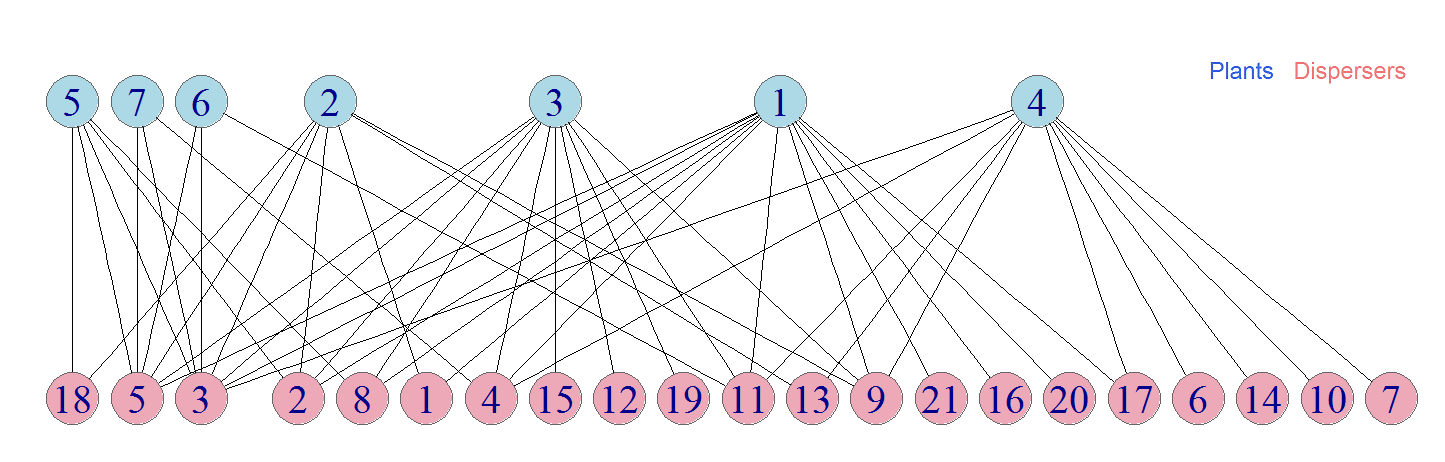
\includegraphics[scale=0.33]{Figures/VIS_bipartito_SD_001.png}
\caption{Diagrama bipartito de una red de dispersores en New Jersey \cite{baird1980selection}.}
\label{fig:VIS_bipartito_SD_001}
\end{figure}

En el ejemplo de la figura \ref{fig:VIS_bipartito_SD_001} la red es pequeña, puede distinguirse el núcleo de plantas más conectadas (de la $1$ a la $4$) y los enlaces se ven con claridad. Cuando el número de especies supera unas pocas decenas, la situación cambia de forma radical.

\begin{figure}[h!]
\centering
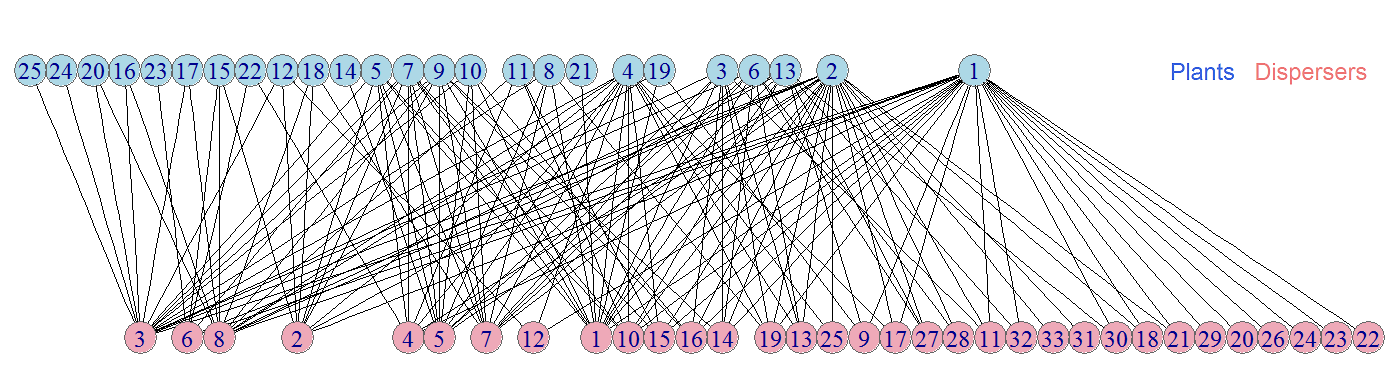
\includegraphics[scale=0.4]{Figures/VIS_bipartito_SD_020.png}
\caption{Red de dispersores en Nava Correhuelas, Sierra de Cazorla, España. Compilada por Pedro Jordano, no publicada.}
\label{fig:VIS_bipartito_SD_020}
\end{figure}

La red de la figura \ref{fig:VIS_bipartito_SD_020} tiene $58$ especies y $150$ enlaces, frente a $28$ especies y $50$ enlaces de la anterior. Es una red de dimensiones moderadas, pero ya es muy complicado seguir los detalles del gráfico. A pesar de ello, algunos autores consiguen resultados excelentes con redes de dimensiones similares a las de este segundo ejemplo, jugando con formas, colores y tamaños \cite{dakos2014critical}. Cuando se llega al centenar de especies, la zona central degenera en una mancha en la que es imposible distinguir los enlaces. Por este motivo, en la literatura sobre mutualismo no aparecen gráficos de redes grandes. 

La matriz de interacción ofrece una visión más rica si los nodos se ordenan de la forma adecuada. Colocando los más conectados en la parte superior izquierda, es fácil localizar el núcleo de especies generalistas. Con redes pequeñas como la del primer ejemplo, el resultado es muy satisfactorio.

\begin{figure}[h!]
\centering
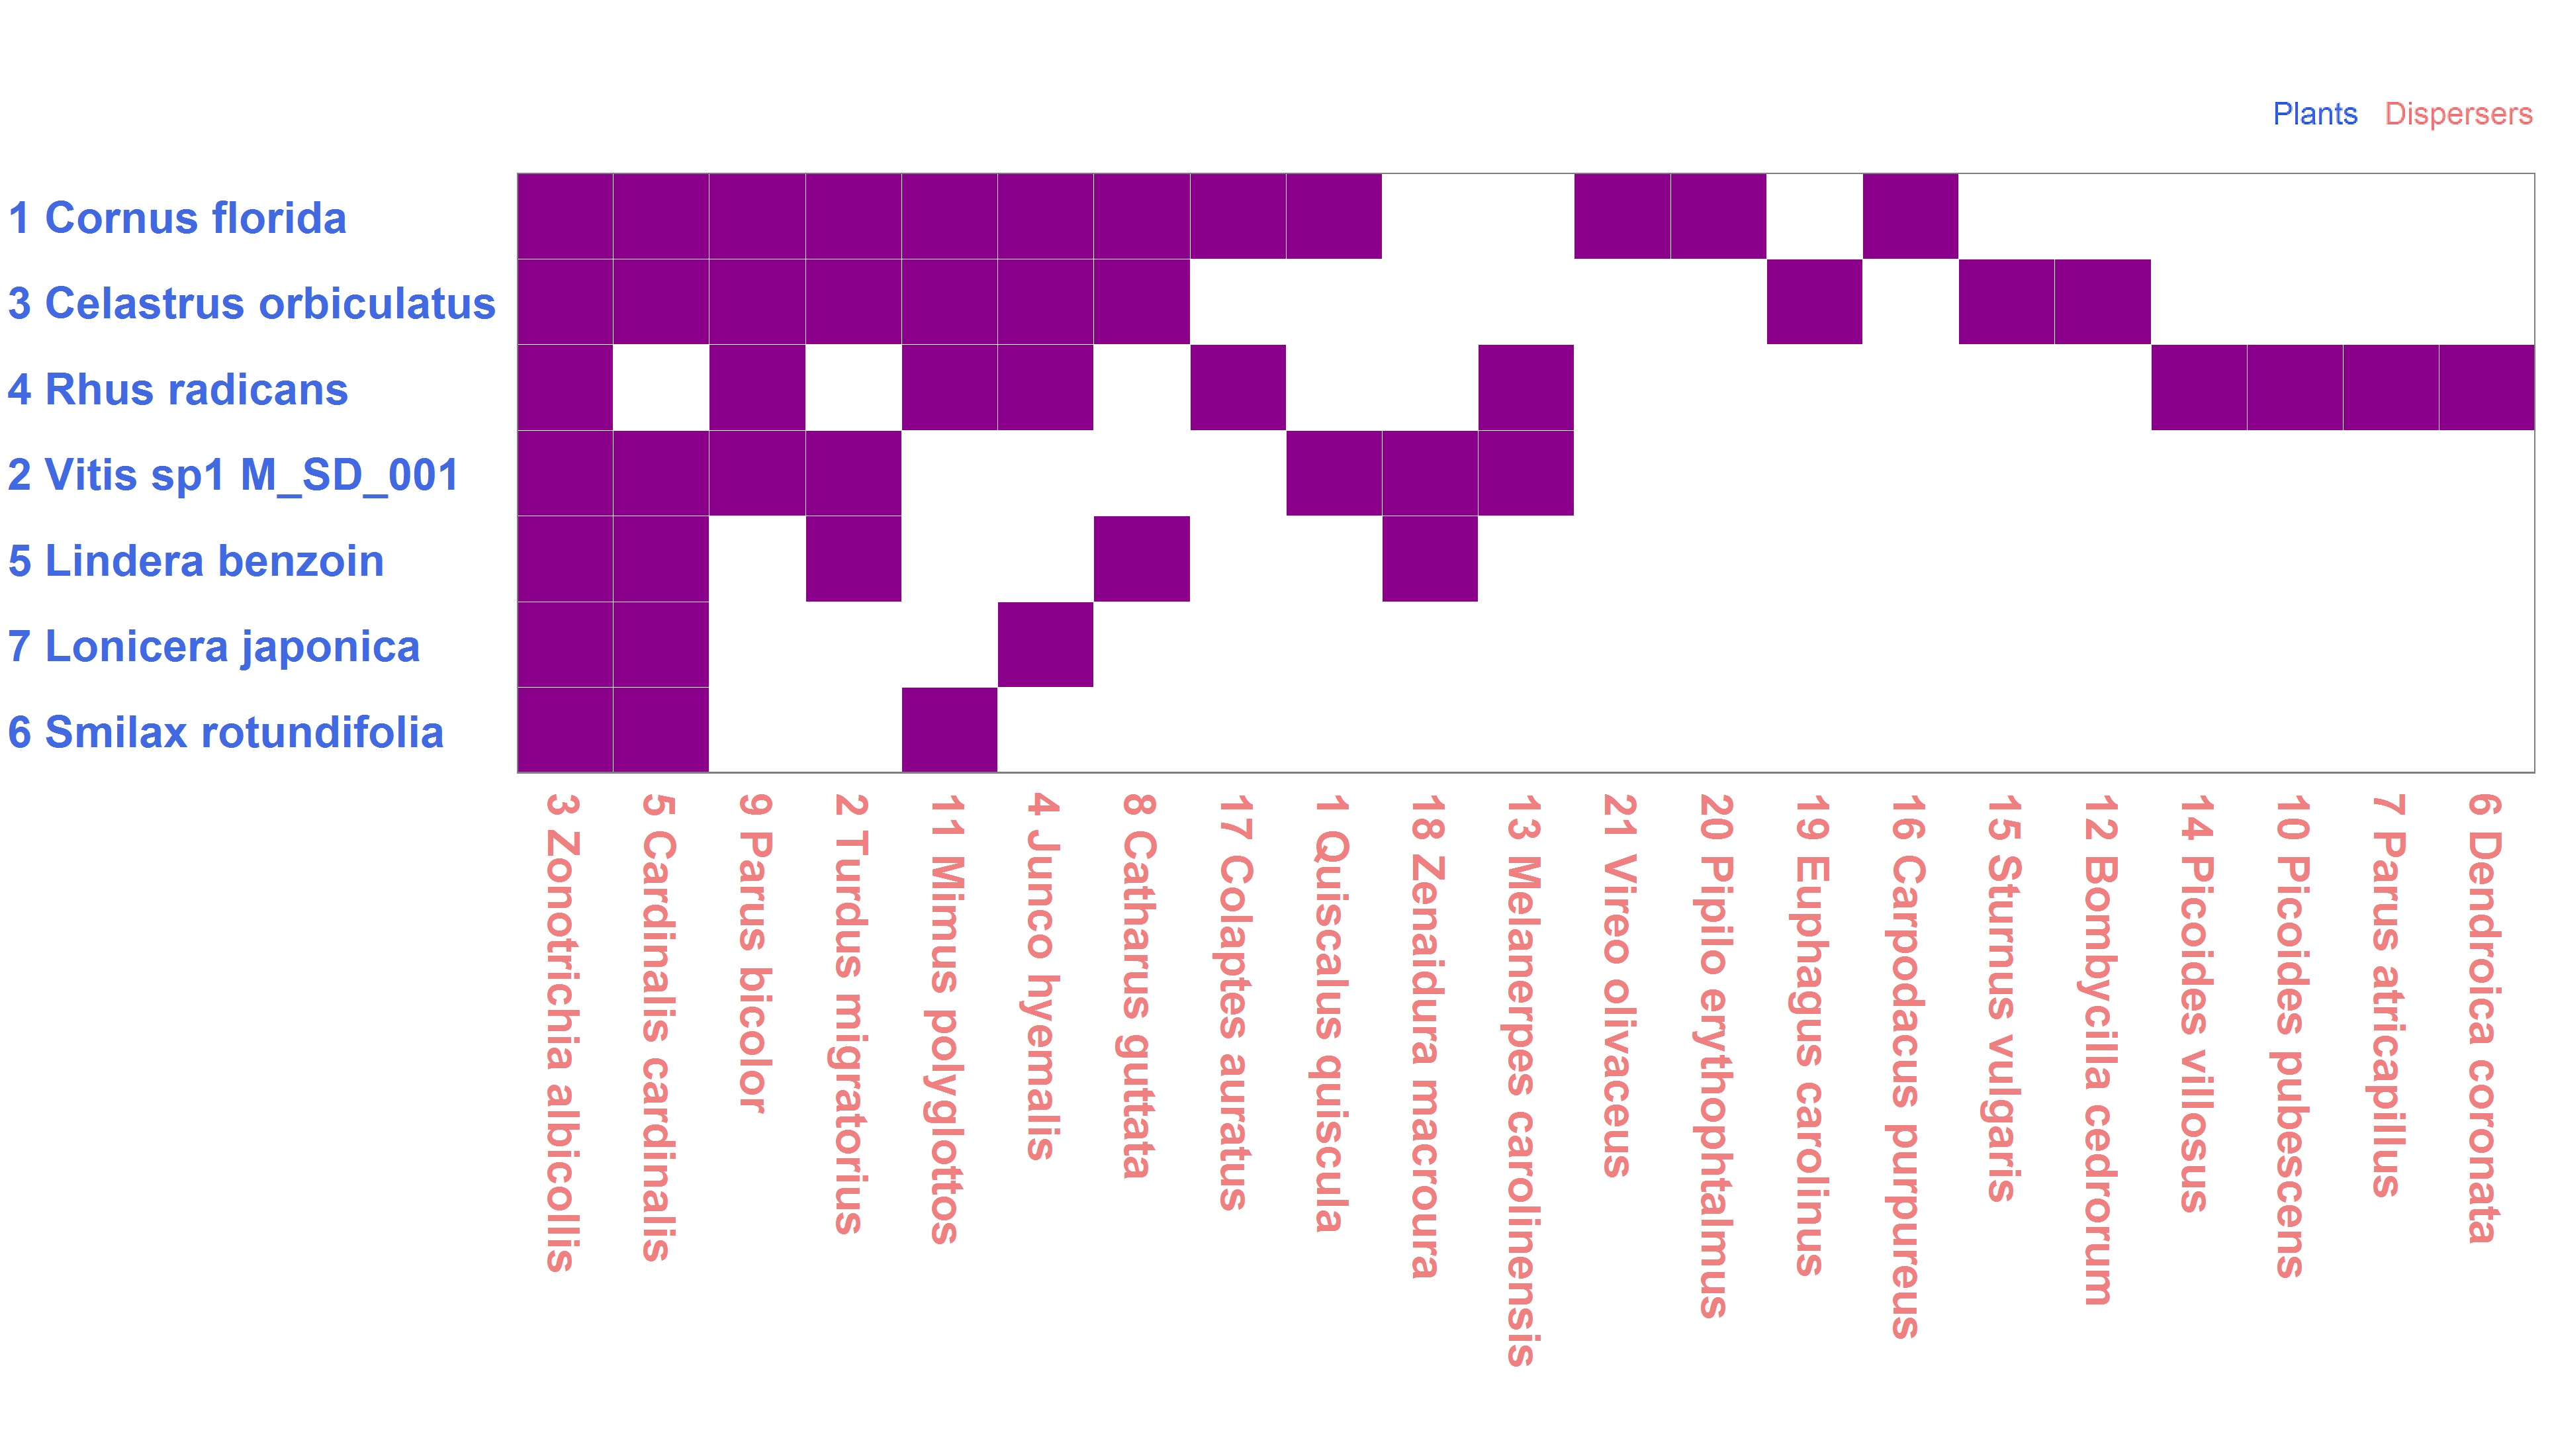
\includegraphics[scale=0.4]{Figures/VIS_matrix_SD_001.png}
\caption{Matriz de interacción de una red de dispersores en New Jersey \cite{baird1980selection}. Las casillas coloreadas indican la existencia de enlace.}
\label{fig:VIS_matrix_SD_001}
\end{figure}

Por el contrario, la matriz de interacción se vuelve también muy confusa para redes grandes, como muestra la figura \ref{fig:VIS_matrix_PL_001}.

\begin{figure}[h!]
\centering
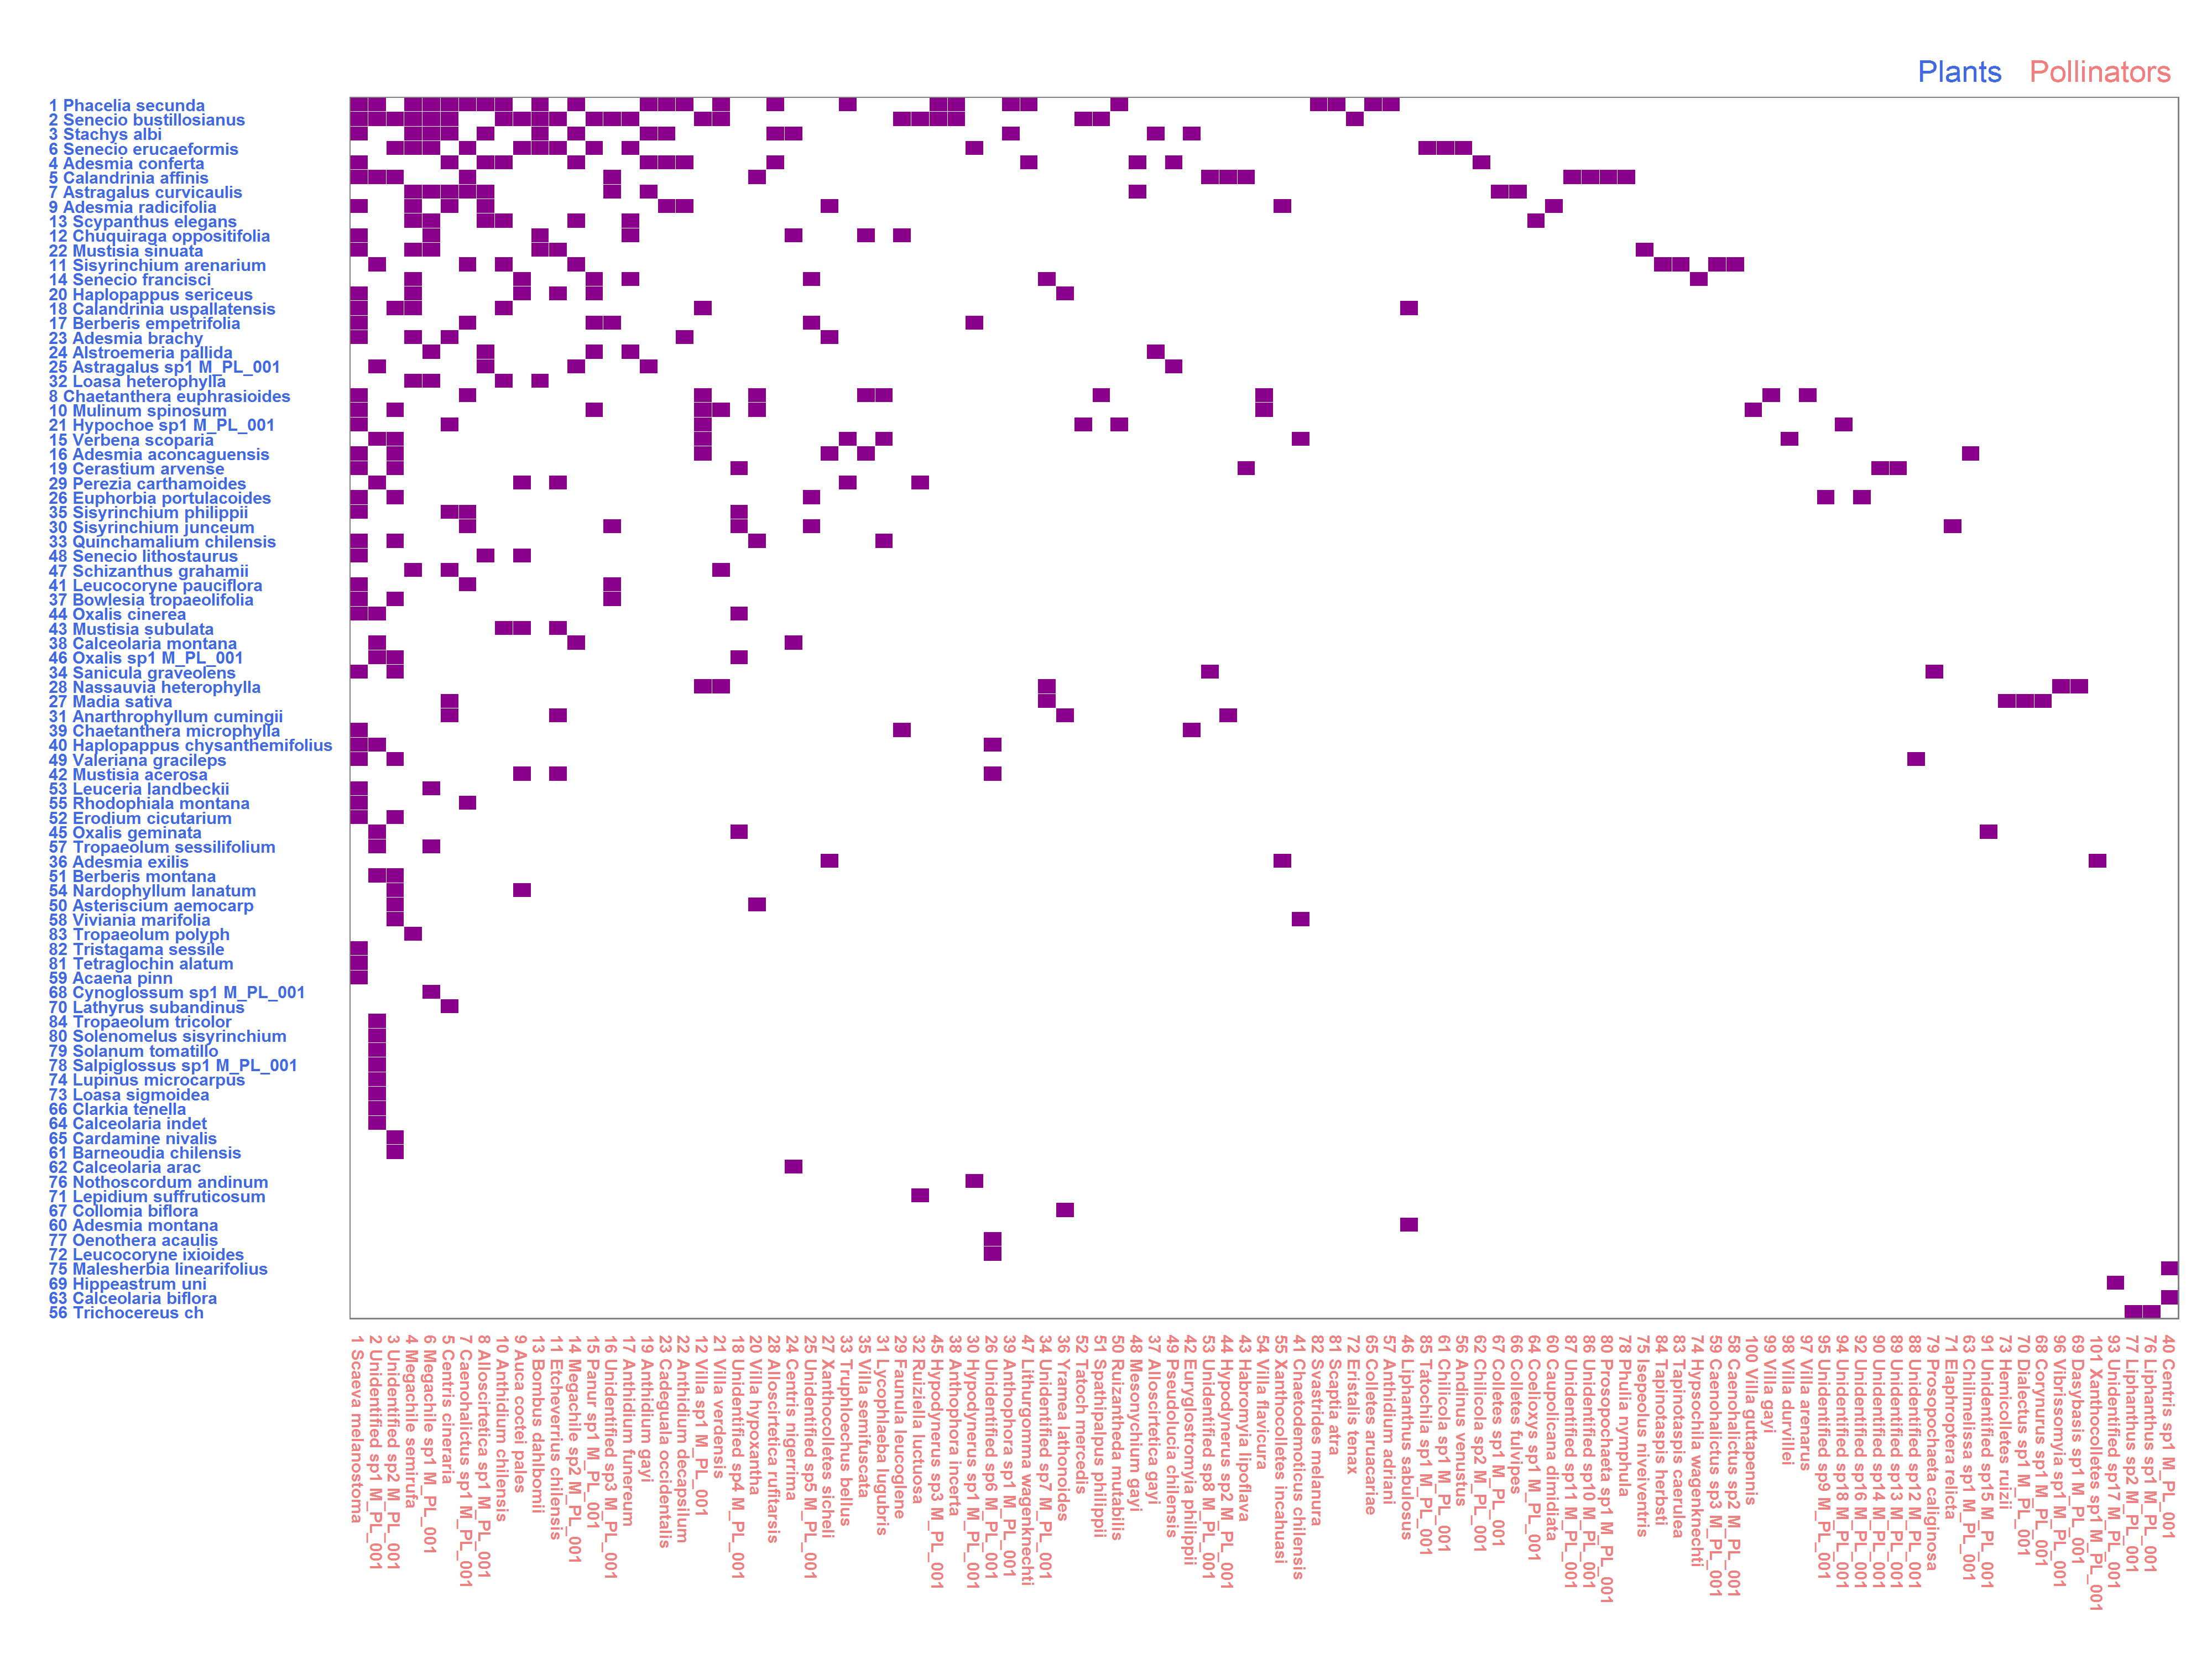
\includegraphics[scale=0.4]{Figures/VIS_matrix_PL_001.png}
\caption{Matriz de interacción de una red de polinizadores en Los Andes, Chile \cite{arroyo1982community}.}
\label{fig:VIS_matrix_PL_001}
\end{figure}


\section{Visualizaciones basadas en \textit{k-magnitudes}}

En este apartado se describen dos nuevos tipos de visualización que se basan en las \textit{k magnitudes} definidas en el capítulo anterior: el diagrama polar y el diagrama zigurat.

\subsection{El diagrama polar}

El diagrama polar se inspira en el \textit{fingerprint plot}, desarrollado por Álvarez-Hamelin \textit{et al} y que se basa en la descomposición \textit{k-core} \cite{alvarez2005k}. Los autores emplearon la técnica para reducir la información y poder visualizar redes muy grandes con índice $k$ máximo del orden de varias decenas. Los nodos se ubican de manera concénrica, a una distancia inversamente proporcional a la \textit{k-shell} a la que pertenecen. No se representan todos los enlaces, solo los más pesados. Una versión más evolucionada no utiliza los nodos sino las \textit{k-shell} que se disponen en espiral \cite{barbera2015critical}.

\begin{figure}[h!]
\centering
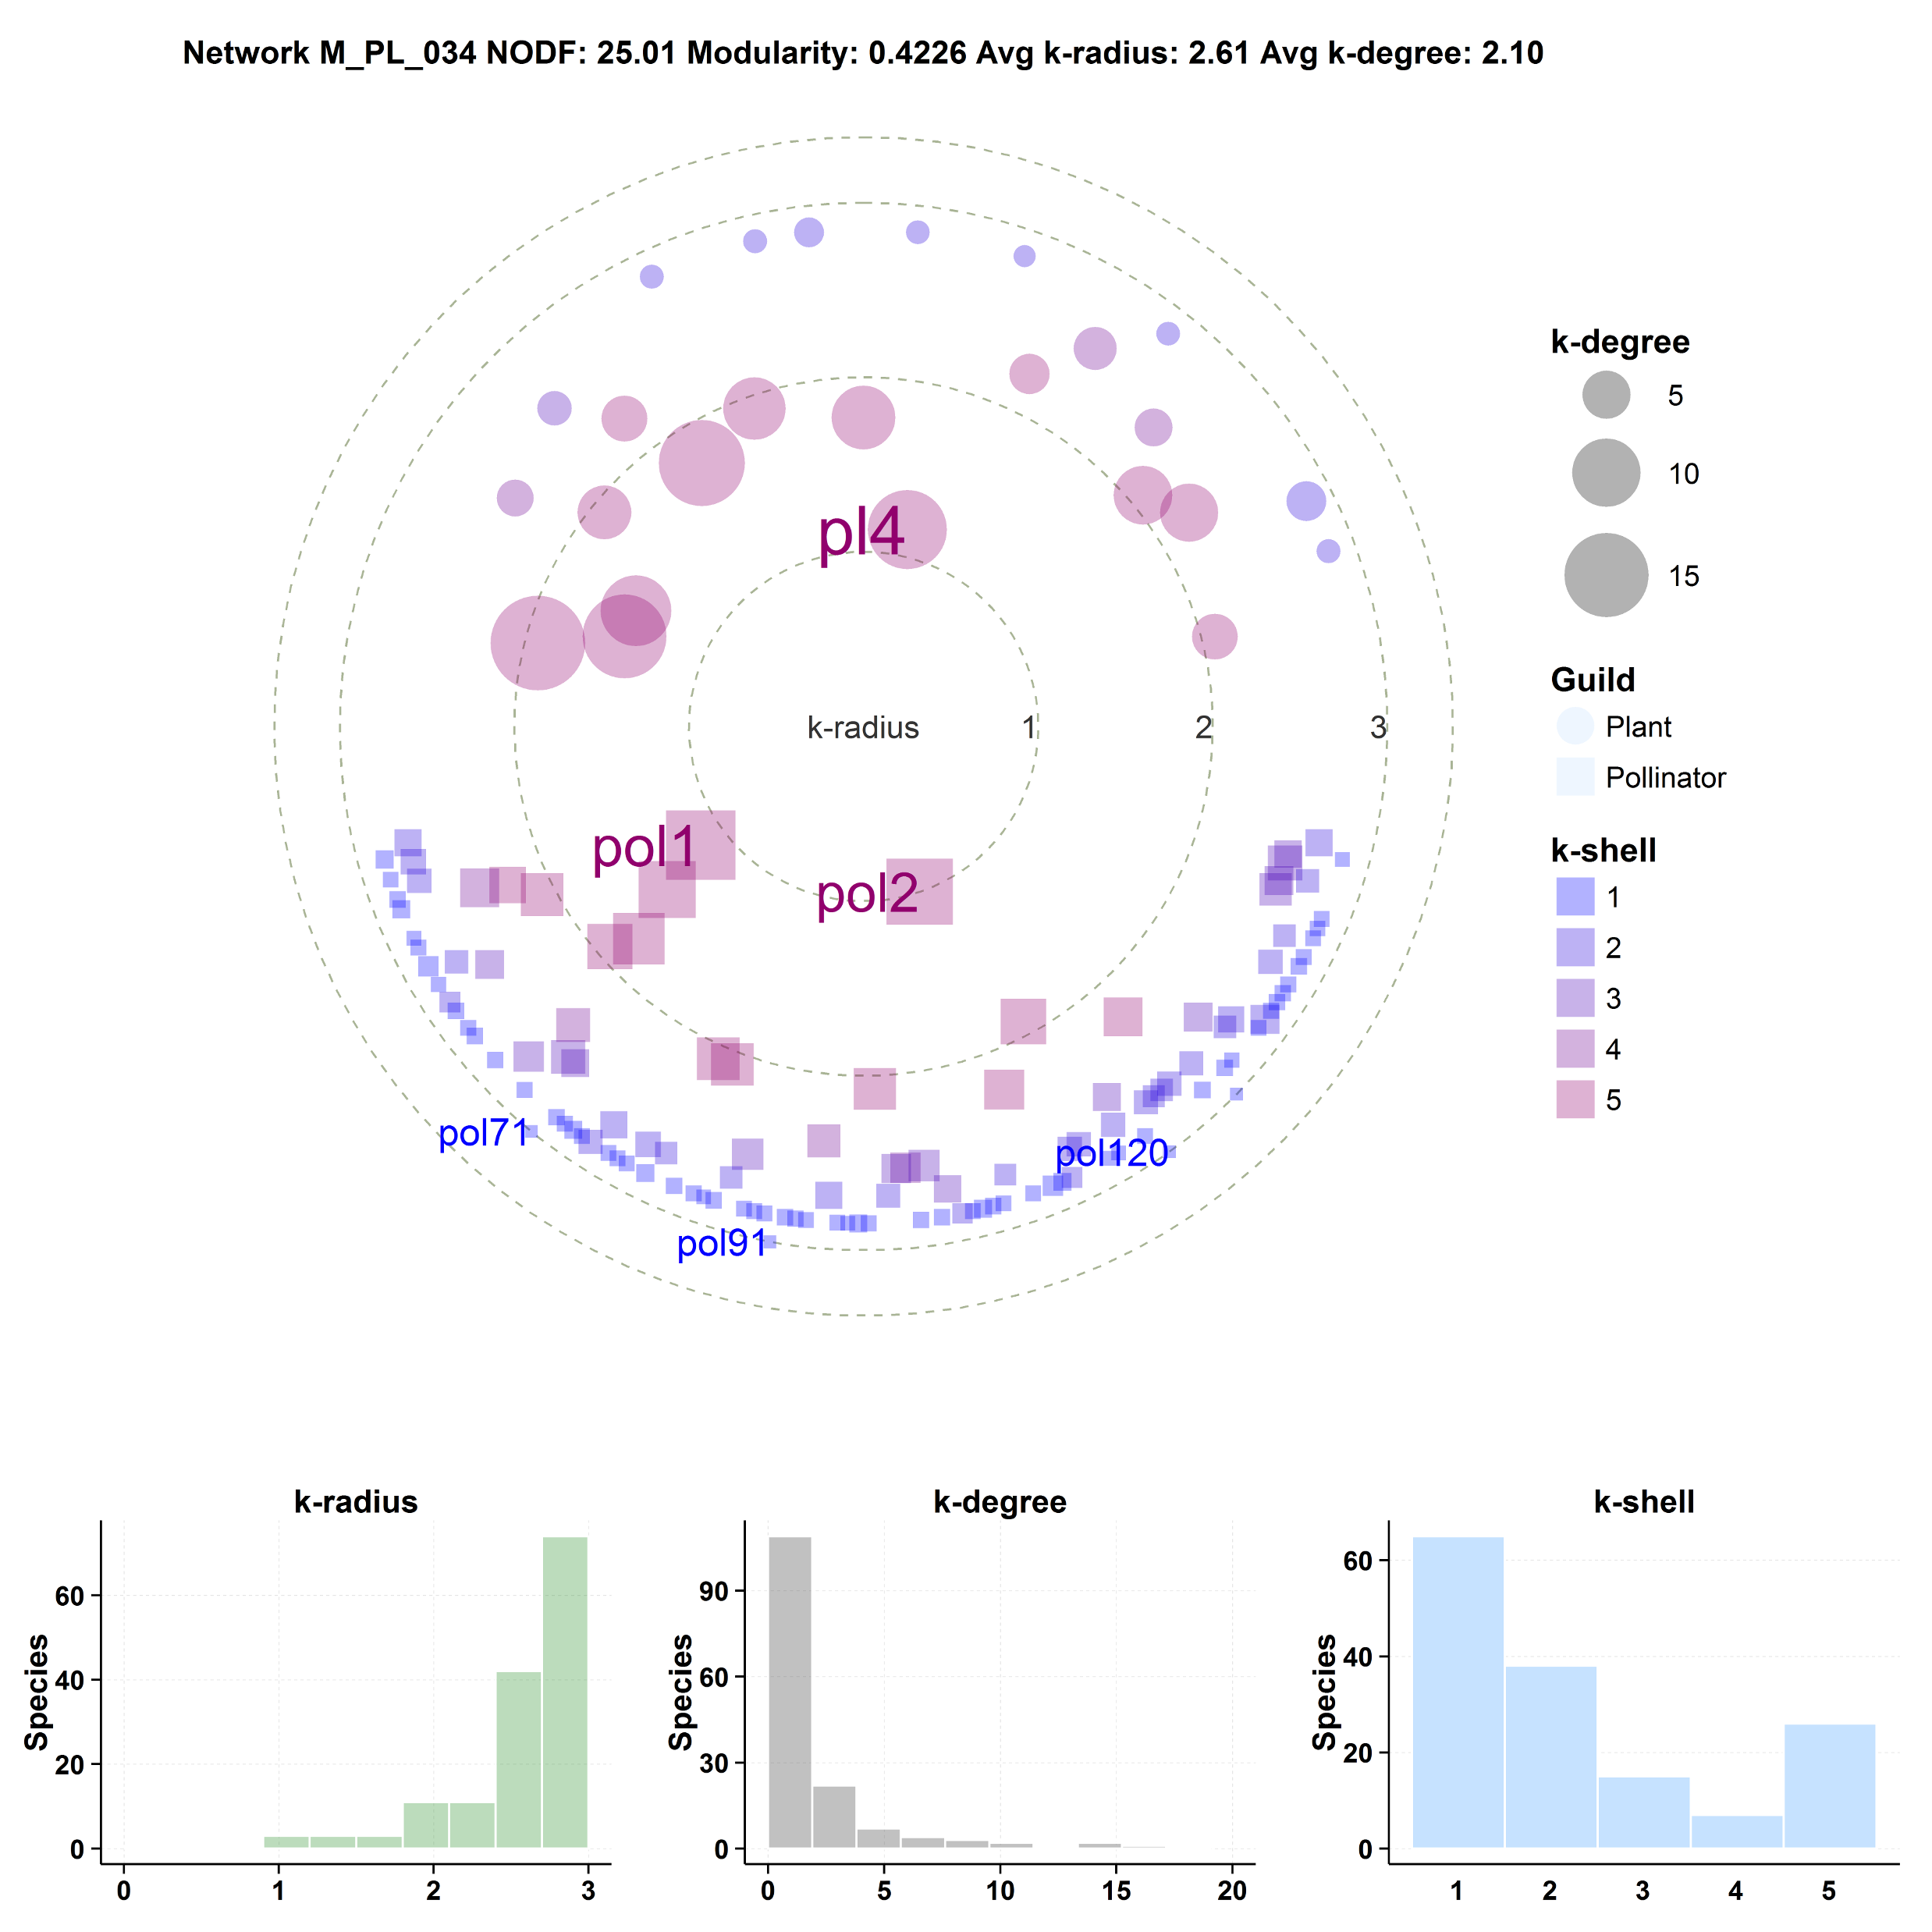
\includegraphics[scale=0.6]{Figures/VIS_M_PL_034_polar.png}
\caption[PolarExample]{Diagrama polar de una comunidad de polinizadores en la isla de Chiloé (Chile) \cite{smith2005diversity}.}
\label{fig:VIS_M_PL_034_polar}
\end{figure}

En el diagrama polar se conserva la idea de diagrama concéntrico y la coloración en función del \textit{k-shell}, pero el difiere en todo lo demás de los dos mencionados. Para empezar, la red es bipartita. Cada clase se sitúa en un de los semiplanos y se utiliza la forma de los nodos para remarcar esta diferencia. El centro de cada especie se sitúa a una distancia $k_{radius}$ del origen de coordenadas, recordemos que el valor mínimo de esta magnitud es $1$. El ángulo se distribuye al azar por el algoritmo de representación para evitar al máximo la superposición de nodos. El área es proporcional al $k_{degree}$ y el color, propio de la \textit{k-shell}. Los enlaces no se representan.

Se puede elegir incluir los nombres de todas las especies, de ninguna, o de un pequeño número, por defecto las tres más centrales y las tres más alejadas. Adicionalmente, el usuario puede decidir que se añadan los histogramas de las tres \textit{k-magnitudes}, que contienen información muy valiosa.

La figura \ref{fig:VIS_M_PL_034_polar} es la representación polar de una red de polinizadores, que hemos elegido por ser una red mutualista tipo tanto por tamaño, anidamiento, modularidad y valores de las \textit{k magnitudes}, todos ellos no demasiado alejados de la media (tabla \ref{table:table_results}). El histograma de la distribución por \textit{k shells} tiene forma de bañera, muy repetido en estas redes. Hay unos pocos nodos domninantes y centrales, de índice $k = 5$ y un número importante de especies en las \textit{shells} exteriores. Es una red de elevada asimetría ($0.66$, véase tabla \ref{table:table_rewiring}).

La utilidad del diagrama polar se descubre al comparar varias redes, incluso si son de tamaños muy dispares. En la figura \ref{fig:VIS_Modvskdegree3}, se han escogido tres redes situadas en ambos extremos y en el centro del diagrama \ref{fig:ESTATICA_corrfigs} (derecha). La red de polinizadores $PL\_010$  tiene un valor de $Modularity$ bajo $(0.25)$, y alto el de $\overline {k}_{degree}$ $(4.57)$. El diagrama polar muestra la estructura en capas del mutualismo. Esta es mucho más evidente en la red $SD\_007$ ($Modularity:    0.28$, $\overline {k}_{degree}: 2.34$). La distribución de $\overline {k}_{degree}$ es más abrupta, con dos especies muy dominantes. La imagen transmite la idea de que esta una red tiene una mayor organización jerárquica que $PL\_010$.

La red $PL\_021$ es grande y fuertemente modular ($Modularity: 0.57$, $\overline {k}_{degree}: 1.23$). La distribución de $\overline {k}_{degree}$ es aun más abrupta. Se ha incluido en la parte inferior izquierda la distribución de densidades que ya aparecía en la figura \ref{fig:ESTATICA_density_plots} porque la escala logarítmica en el eje horizontal permite ver mejor las diferencias.

\begin{figure}[h!]
\centering
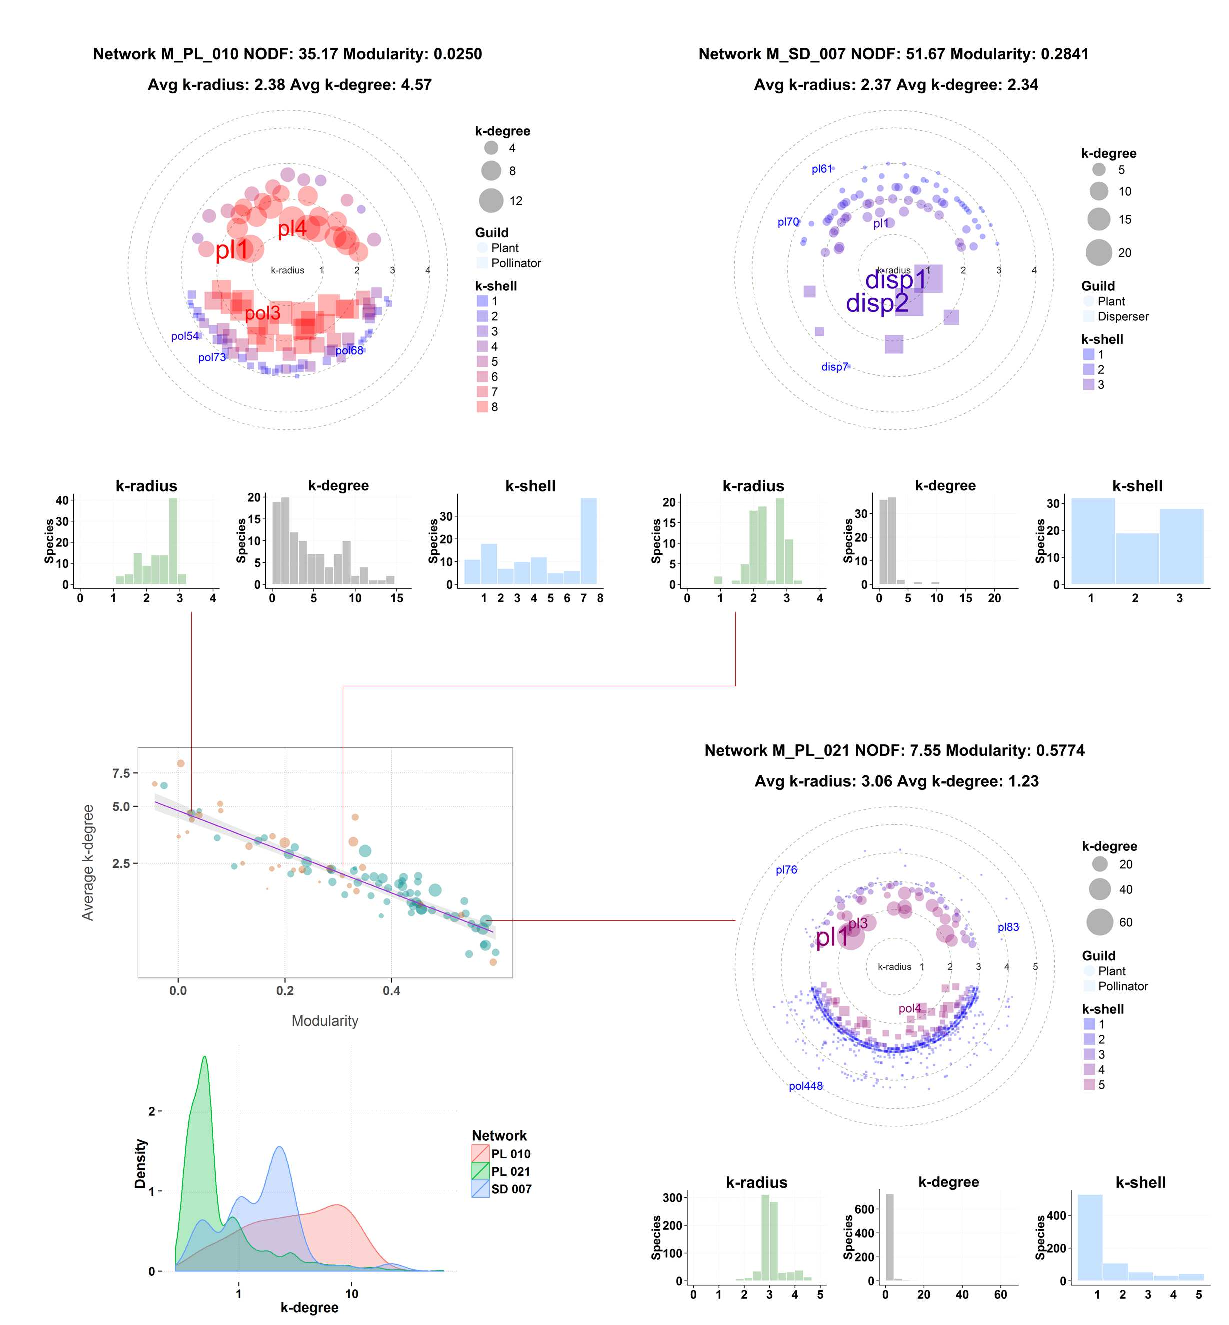
\includegraphics[scale=0.75]{Figures/VIS_Modvskdegree3.PDF}
\caption[PolarExample]{Comparación de tres redes mediante sus diagramas polares.}
\label{fig:VIS_Modvskdegree3}
\end{figure}

A pesar de que el diagrama polar ofrece una nueva visión de las comunidades mutualistas, tiene limitaciones. Como en toda estrategia de reducción de la información hay que renunciar a representar detalles en favor de una mejor visibilidad, en este caso los enlaces. No se trata de un detalle menor, así que se ha desarrollado un segundo tipo de diagrama que los toma como base de su construcción.

\subsection{El diagrama zigurat}

El diagrana zigurat se ha creado para mostrar la estructura de \textit{k shells} de una red bipartita y todos los enlaces entre sus nodos. La idea básica consiste en agrupar las especies en \textit{shells} que se representan como pequeños zigurats\footnote{Según el DRAE: Torre escalonada y piramidal, característica de la arquitectura religiosa asiria y caldea.}. Las dos \textit{shells} máximas se colocan en el eje de simetría horizontal, ligeramente hacia la izquierda. El resto, se distribuyen siguiendo una disposición en forma de almendra, que deja un gran espacio libre para dibujar los enlaces.

\begin{figure}[h!]
\centering
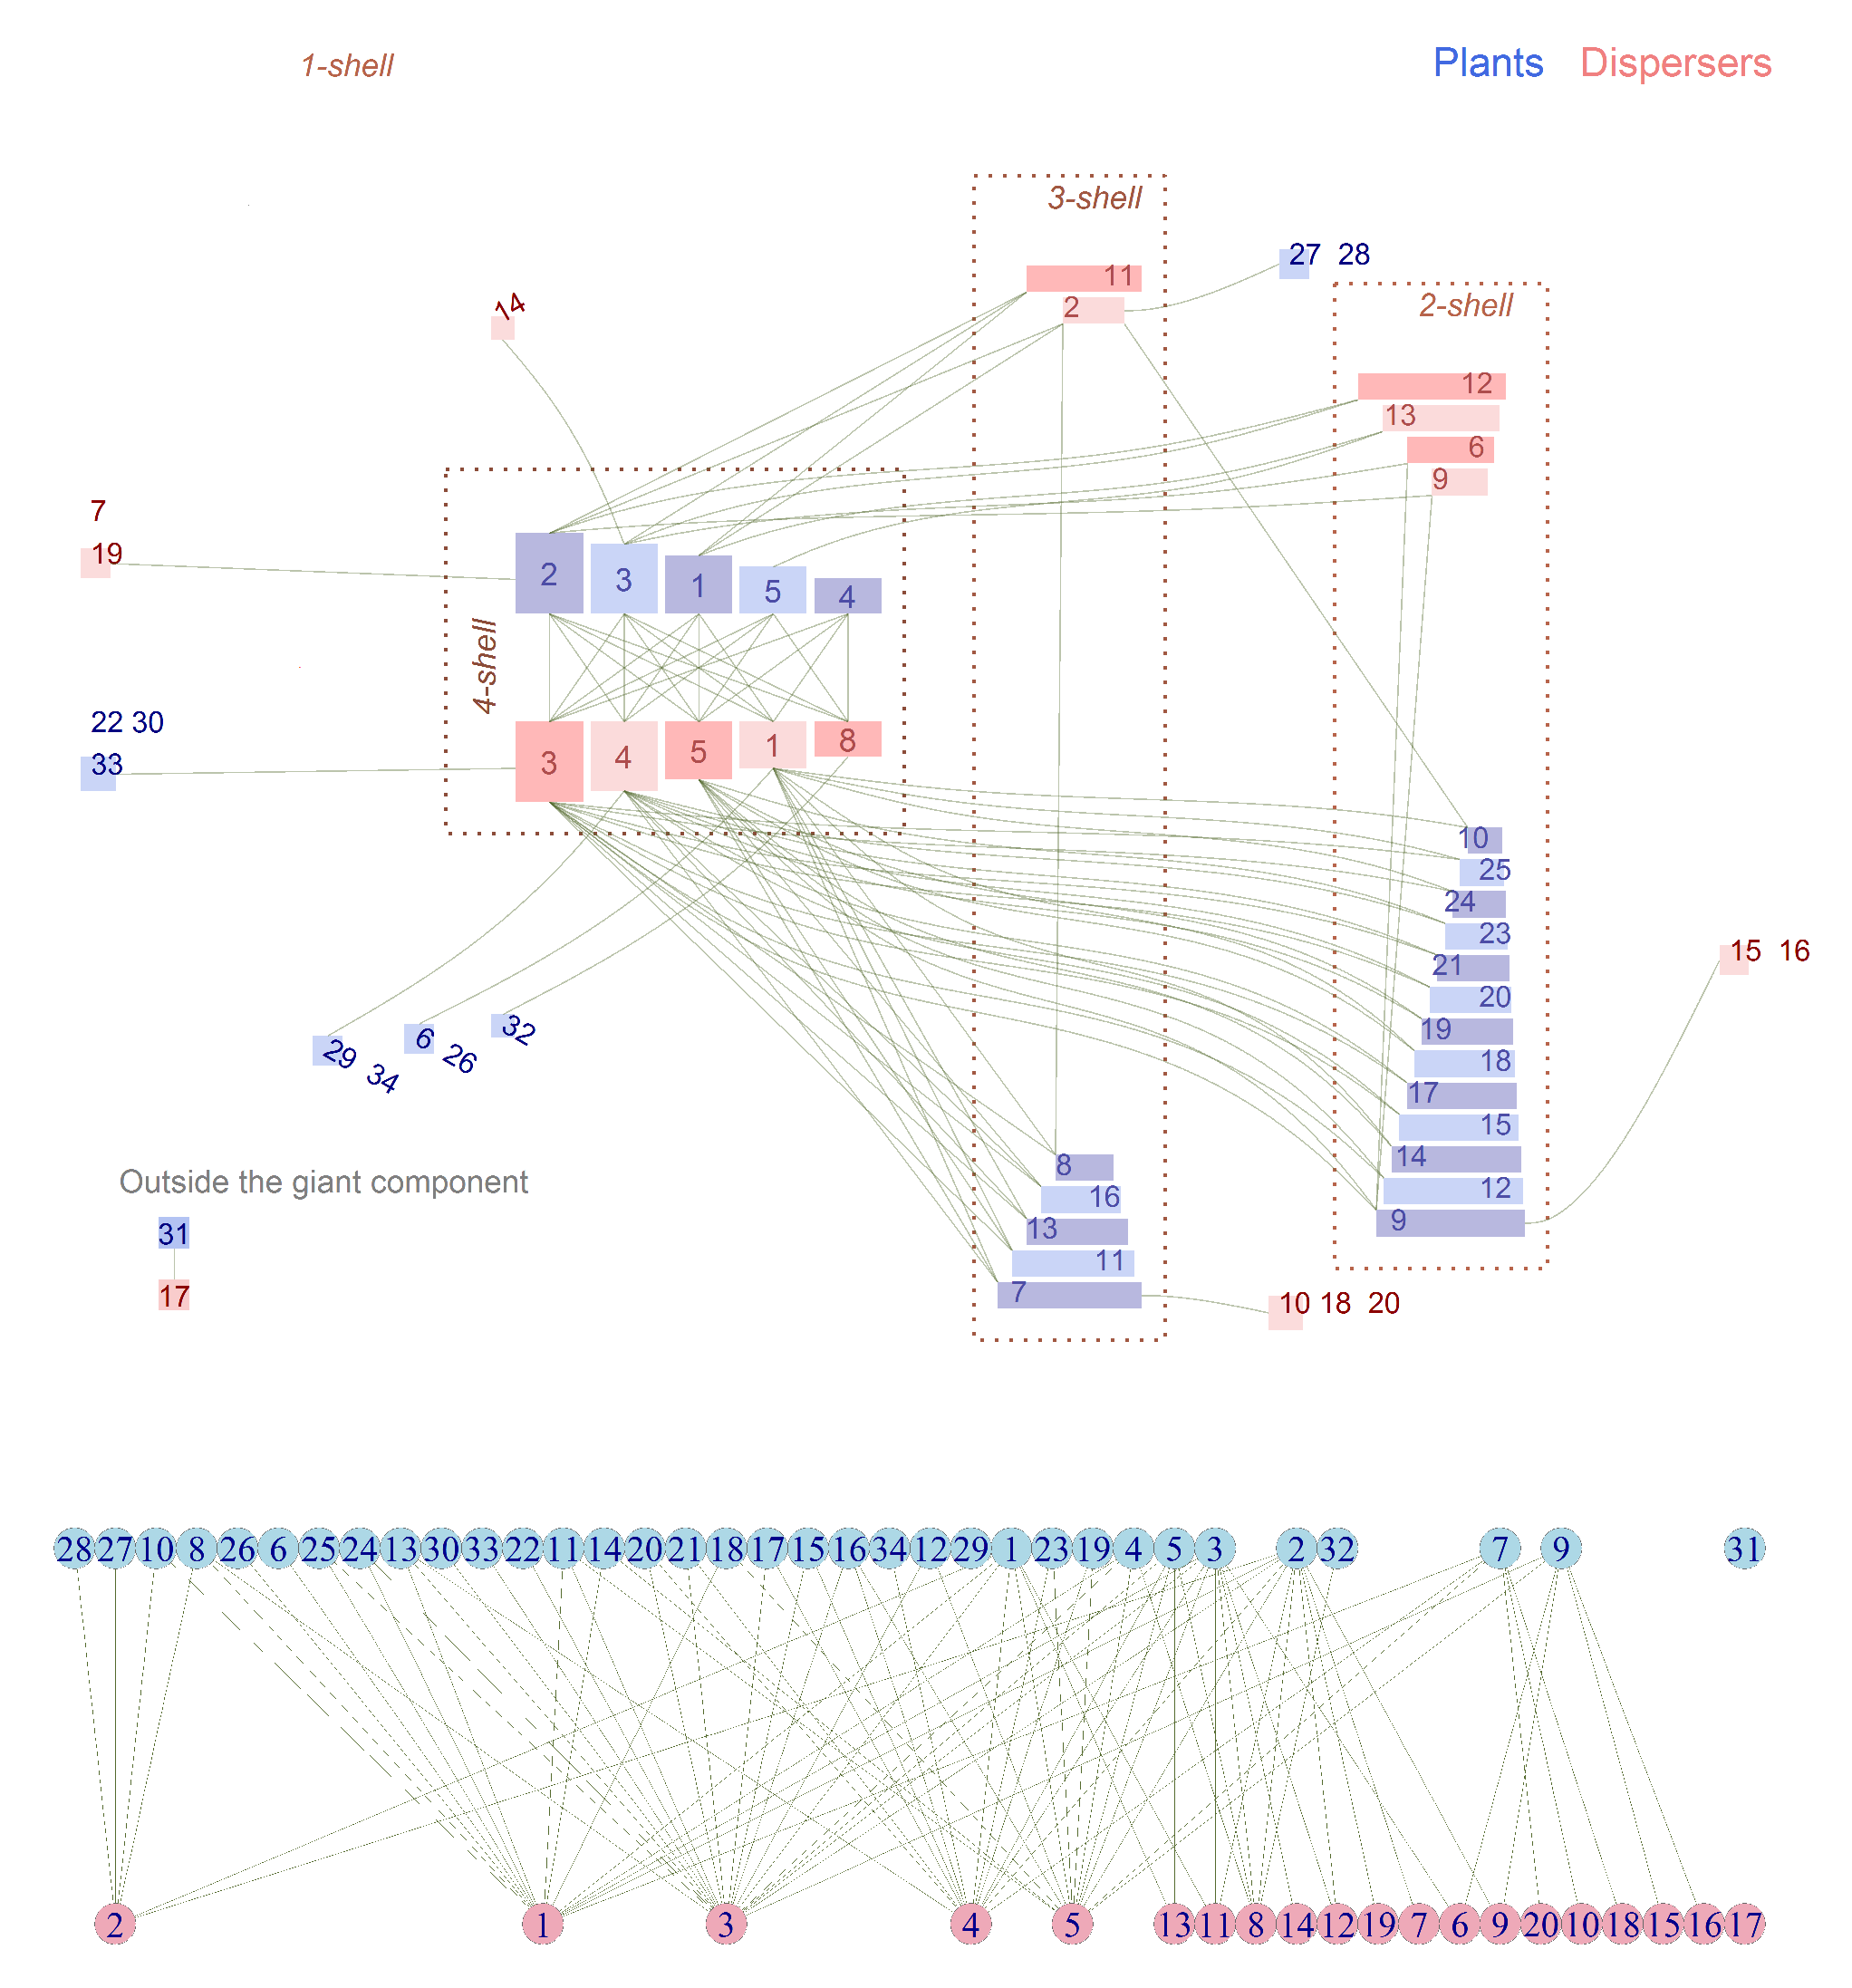
\includegraphics[scale=0.45]{Figures/VIS_ALL_SD_004.eps}
\caption {Diagrama zigurat de una comunidad de aves frugívoras de Puerto Rico  $M\_SD\_004$, con $54$ especies y $95$ enlaces \cite{carlo2003avian}. $\overline k_{radius} = 2,19$; $\overline k_{degree} = 2,37$; $NODF = 39,82$; $Modularity = 0.34$. Abajo el diagrama bipartito.}
\label{fig:ziggurat}
\end{figure}

En la \textit{shell} máxima las especies se ordenan por $k_{degree}$, con el valor mayor a la izquierda. En el resto, se ordenan por $k_{radius}$, correspondiendo la base del zigurat a la especie de menor $k_{radius}$.

Las especies de la \textit{1-shell} se disponen como una nube el torno a la almendra central. Si, como sucede a menudo, varias especies de esta \textit{shell} comparten enlace, se dibujan de forma agrupada y con un único enlace.

En algunas redes, los autores han incluido observaciones de especies que no están conectadas con la componente gigante. En ese caso, se representa el fragmento inconexo, pero no se tiene en cuenta para la \textit{k descomposición}.

Por último, es importante recalcar que en el diagrama zigurat, las áreas no transmiten información sobre tamaños de la población.

La red de la figura \ref{fig:ziggurat} es de pequeño tamaño. En el gráfico bipartito todavía se pueden seguir los enlaces individuales. Sin embargo, el zigurat ofrece una visión mucho más rica de la organización con cuatro \textit{shells} internas y una pequeña \textit{1-shell}. Se pueden descubrir con facilidad algunos patrones, como la baja conectividad entre especies de las \textit{shells} de menor índice $k$, o la relativa importancia de la especie dispersora $2$ que en el bipartito aparece en el extremo izquierdo.

\begin{figure}[ht!]
\centering
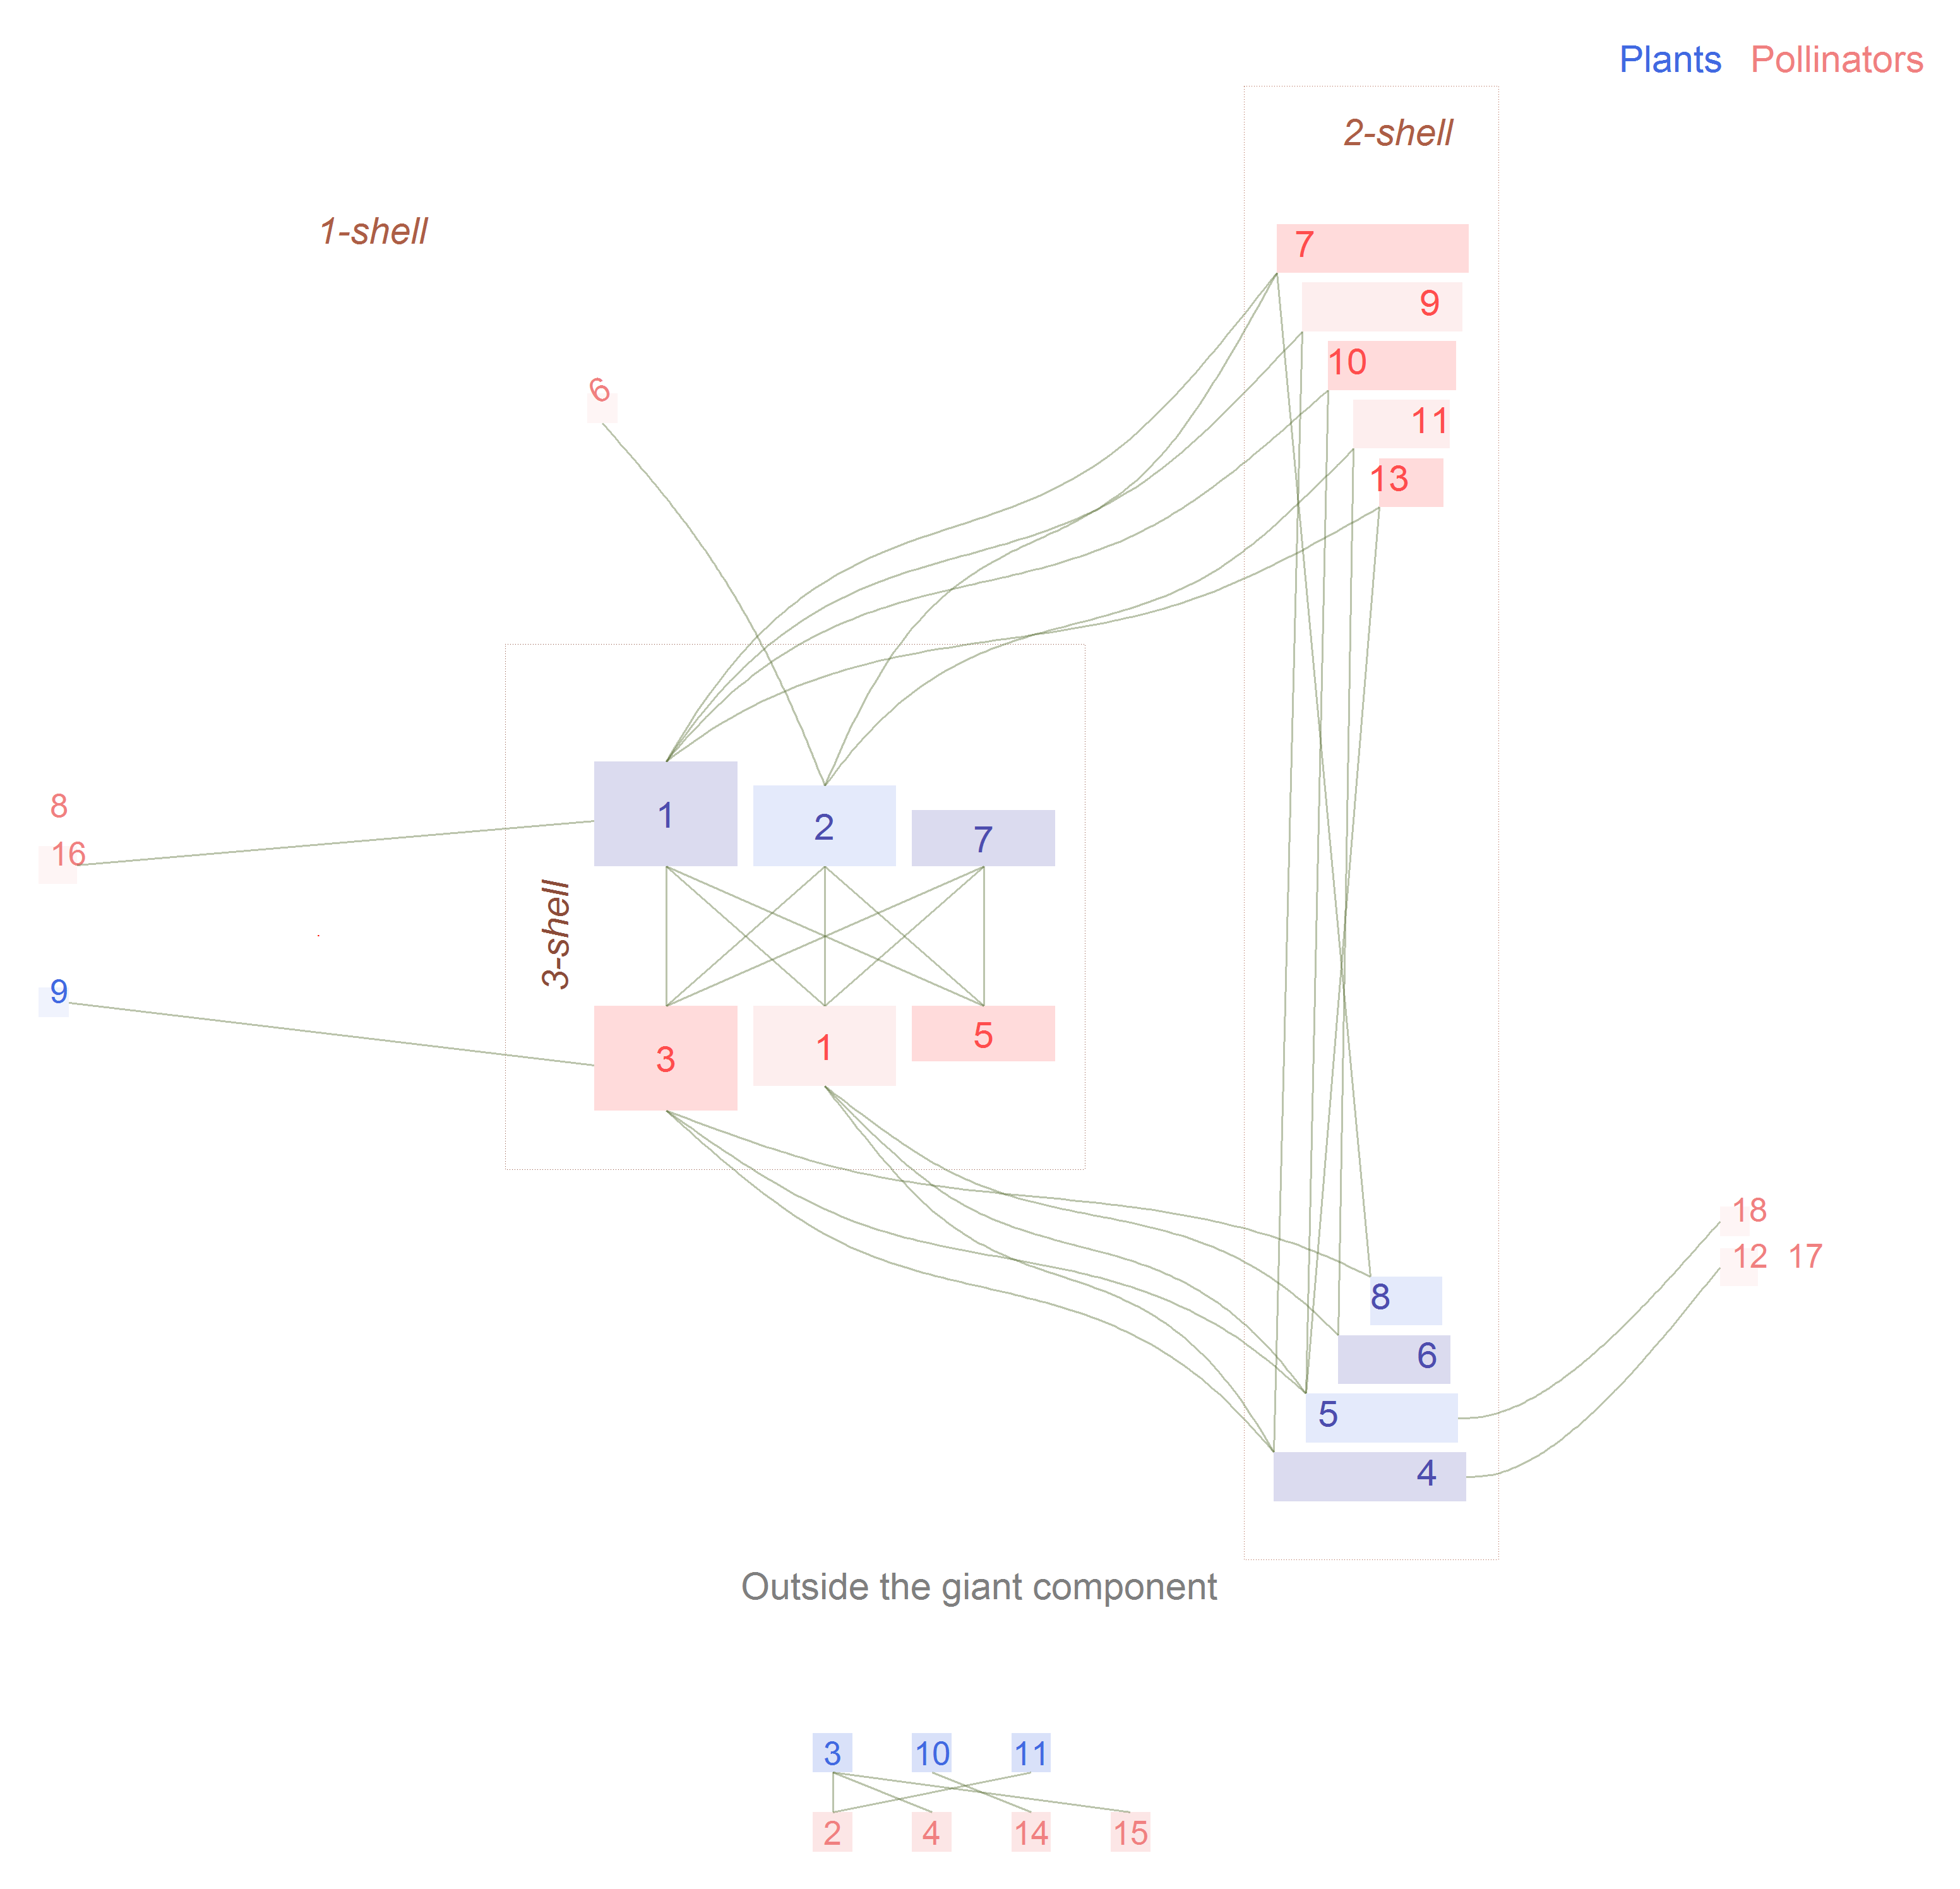
\includegraphics[scale=0.16]{Figures/VIS_zig_pl_024.png}
\caption {Red de polinizadores $M\_PL\_010$, Melville Island, Canada \cite{mosquin1967observations}, con $29$ especies y $38$ enlaces}
\label{fig:VIS_zig_pl_024}
\end{figure}

El diagrama zigurat funciona bien para los tamaños típicos de las redes mutualistas documentadas en la literatura. La red de la figura \ref{fig:VIS_zig_pl_024} es pequeña, muy simétrica y con valores intermedios de $NODF$ y de las \textit{k magnitudes} (véase la tabla \ref{table:table_results}). La especie con mayor $k_{degree}$ $(5,74)$ es la planta $1$. En esta red todas las especies de las \textit{shells} máximas están conectadas entre sí, por lo que sus $k_{radius}$ valen $1,0$, pero esto no tiene por qué suceder siempre. Las más distantes de la $3$-$shell$ (descartando a las que no están conectadas con la componente gigante) son los polinizadores $12$,$17$ y $18$, con  $k_{radius}$ $3,0$, que aparecen conectadas en el extremo derecho al zigurat de la $2$-$shell$ de plantas.


\begin{figure}[h!]
\centering
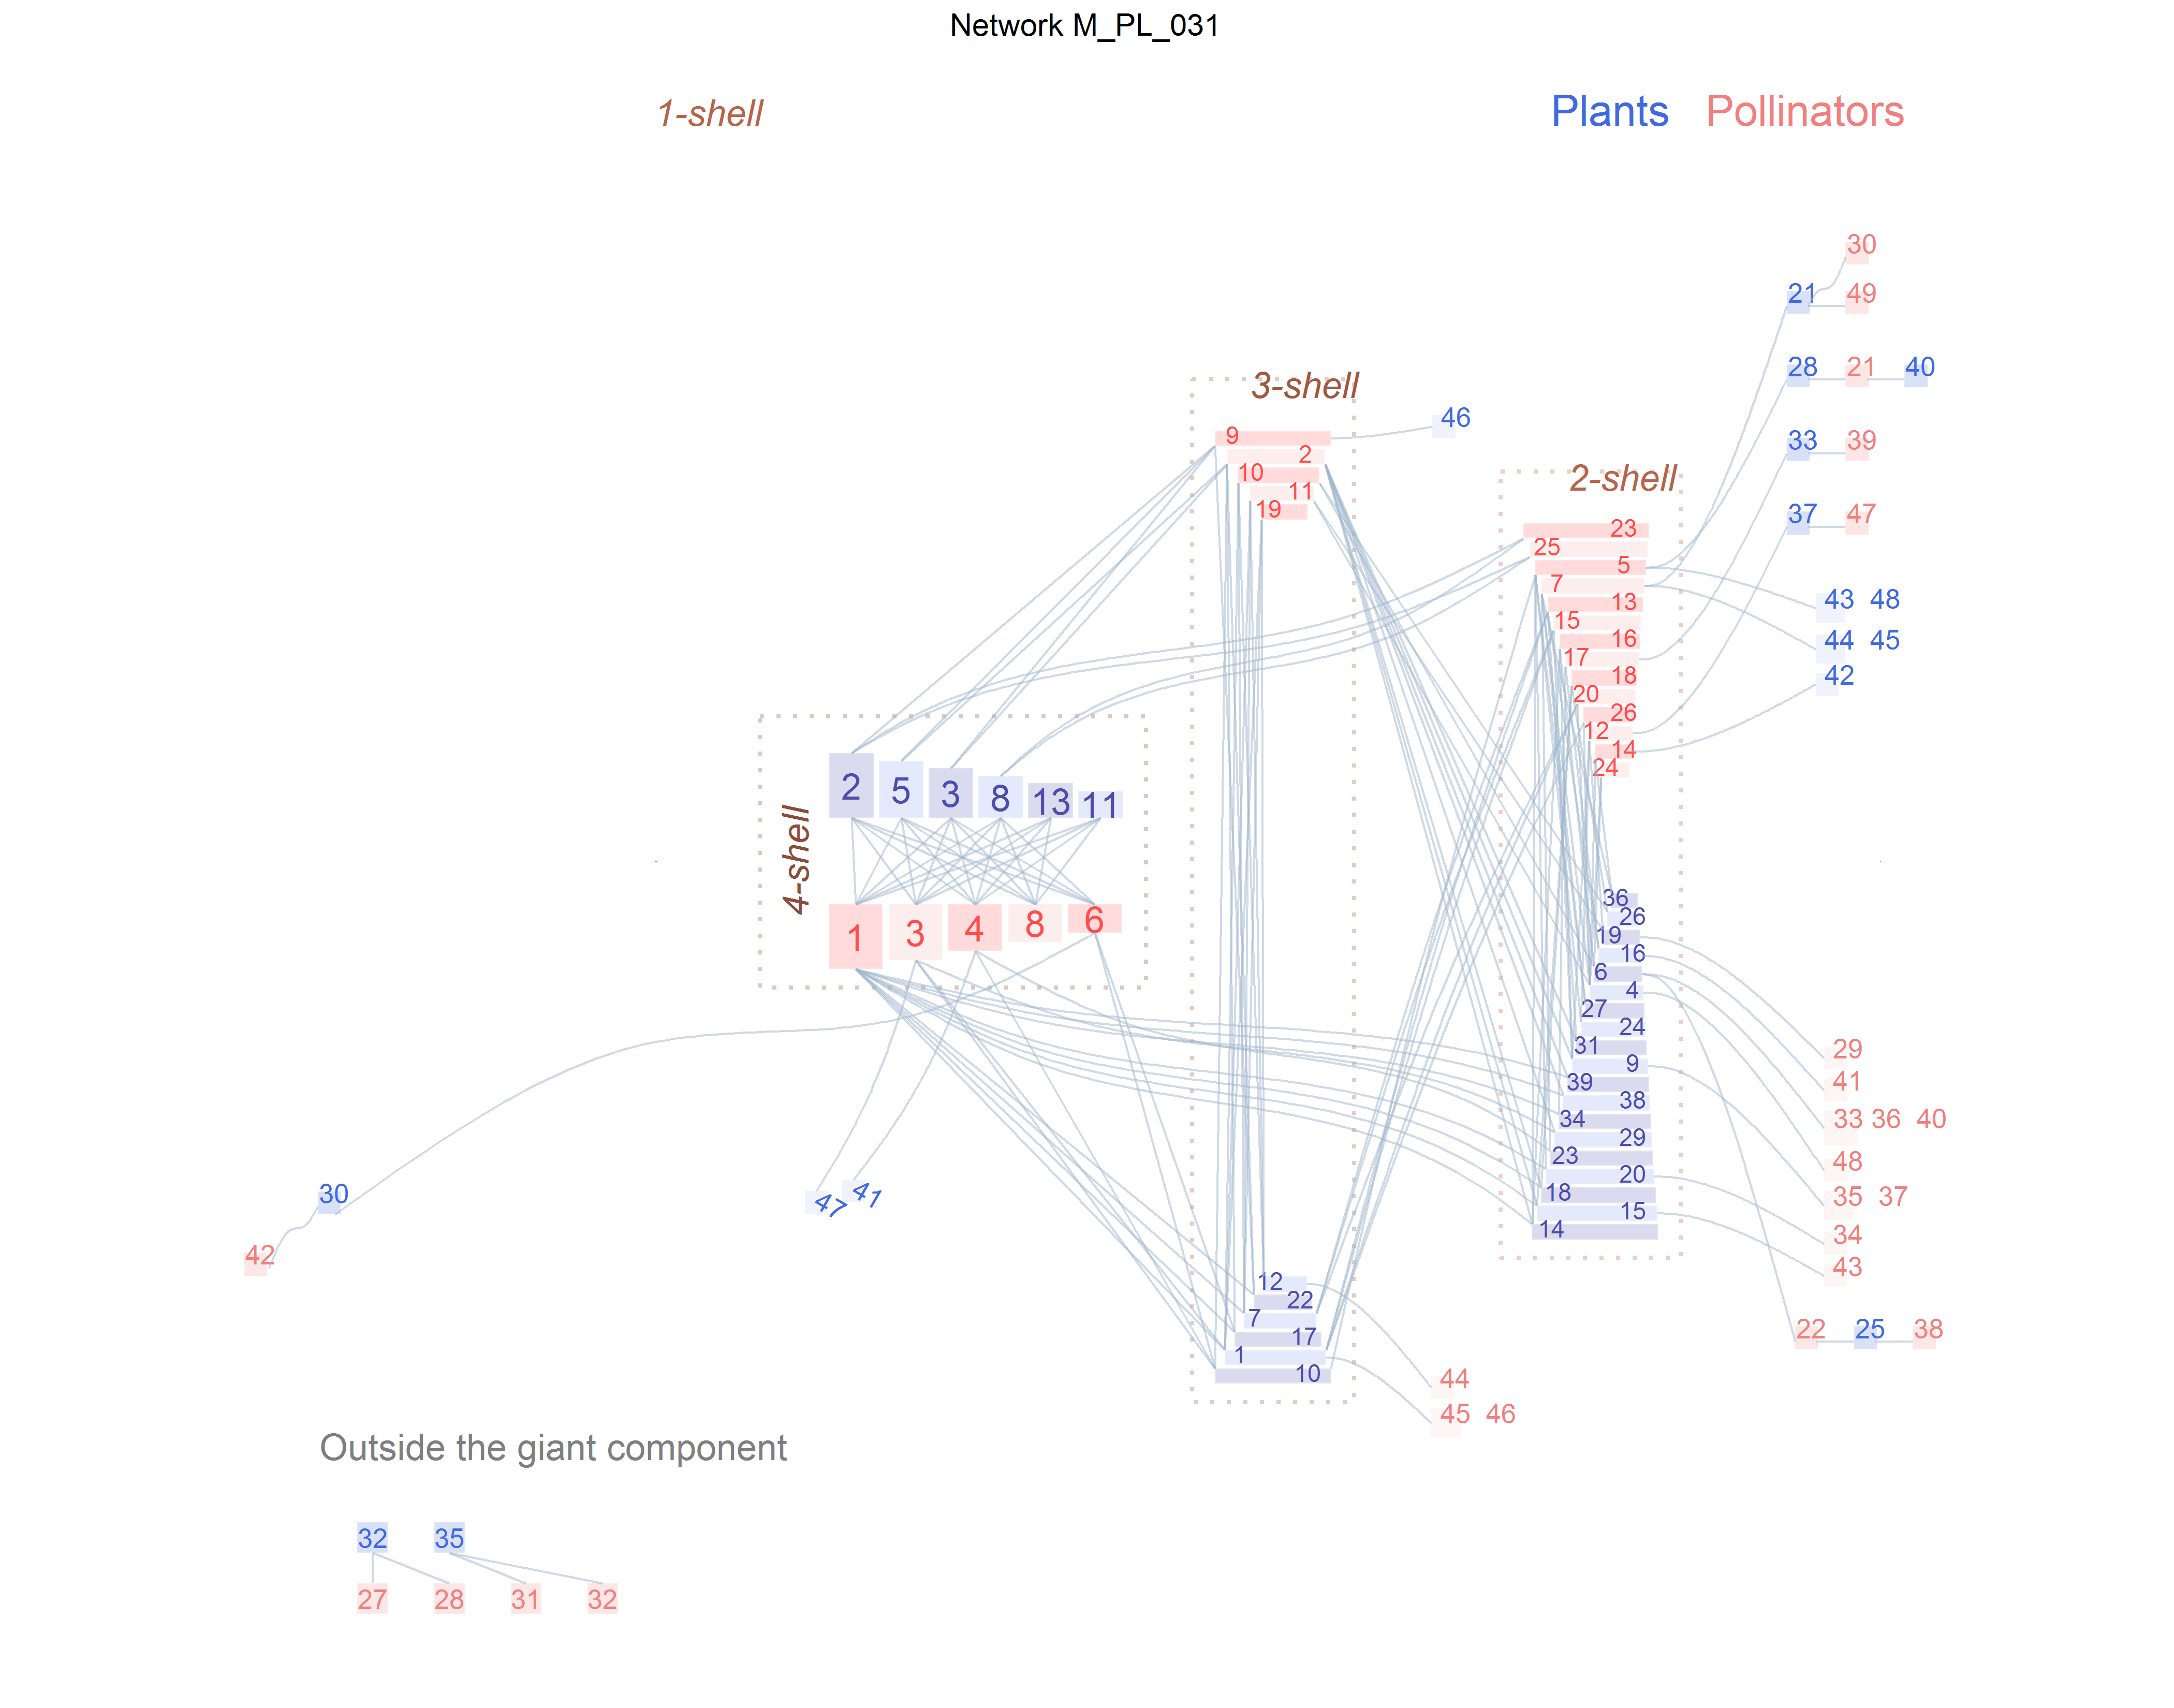
\includegraphics[scale=0.14]{Figures/VIS_M_PL_031_ziggurat.png}
\caption {Red de polinizadores $M\_PL\_031$ del Parque Nacional de Canaima, Venezuela, con $97$ especies y $156$ enlaces \cite{ramirez1989biologia}.}
\label{fig:VIS_M_PL_031_ziggurat}
\end{figure}

La red de la figura \ref{fig:VIS_M_PL_031_ziggurat} es de un tamaño intermedio, y muestra abundancia de especialistas conectadas a otras especialistas, una circunstancia poco común. A diferencia del caso anterior, no todas las especies del las \textit{shells} máximas tienen enlaces directos con todas las de la clase contraria. Así, mientras el $k_{radius}$ del polinizador $1$ o la planta $2$ es $1,0$, el de la planta $13$ es $1,4$ y el del polinizador $6$ es $1.66$ (tabla \ref{table:kmag_pl_031}). La existencia de especialistas ultraperiféricos se traduce en valores elevados del $k_{radius}$, por ejemplo $7.0$ para el polinizador $38$ ó $6.2$ para la planta $25$ que es el primer enlace de su camino más corto hacia el centro de la red.

\begin{figure}[ht!]
\centering
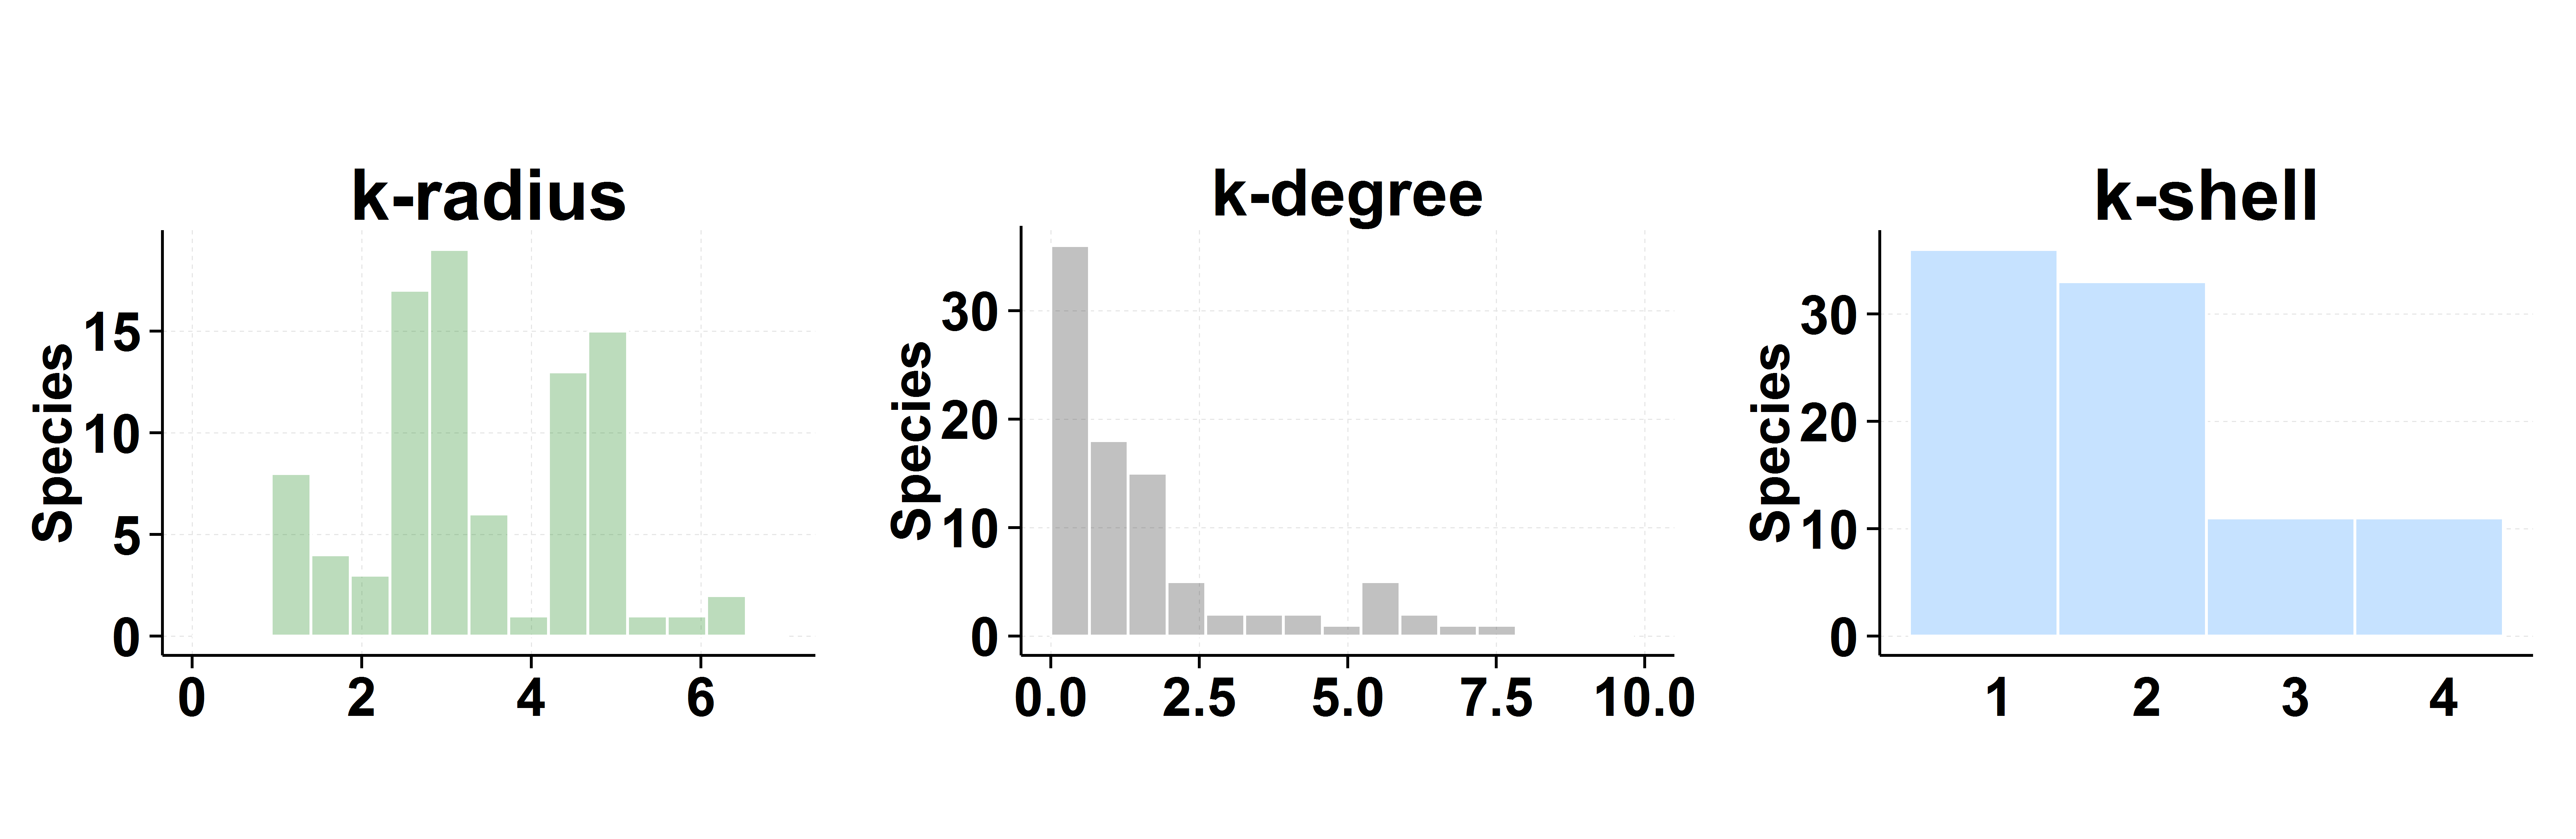
\includegraphics[scale=0.45]{Figures/VIS_M_PL_031_polar.png}
\caption {Histograma de las \textit{k magnitudes} de polinizadores del Parque Nacional de Canaima, Venezuela \cite{ramirez1989biologia}.}
\label{fig:VIS_M_PL_031_polar}
\end{figure}

Estas especies tan alejadas del centro corren el peligro de extinción por arrastre que se describió en el apartado \ref{results_K_constante}. Supongamos que el polinizador número $7$ se extingue por una plaga. En la parte superior derecha de la figura \ref{fig:VIS_M_PL_031_ziggurat} puede verse la tripleta planta $21$, polinizadores $30$ y $49$ que quedarían desconectados de la componente gigante y posiblemente se extinguirían también. En el mejor de los casos, si por el peso de sus enlaces superaran el mínimo vital de la nueva red formada por las tres, podrían sobrevivir aisladas pero mucho más expuestas a cualquier perturbación posterior. Las plantas $44$ y $45$ desaparecerían con seguridad porque el polinizador $7$ es su única especie benefactora. De esta manera, la destrucción de un polinizador podría arrastrar cinco especies más a la extinción. En el diagrama se puede ver también la gran conectividad entre especies de las \textit{shells} de índices $2$ y $3$, que se refleja en un anidamiento bajo y notable modularidad. Por el contrario, la red de la figura \ref{fig:ziggurat} es mucho más anidada, con pocos enlaces que no terminen en la $4$-$shell$ y con un $\overline k_{radius}$ reducido ($2,19$ frente a $3,39$).


El tamaño de una red se puede medir en número de nodos o en número de enlaces, pero es esta segunda cifra la que predomina a la hora de fijar la complejidad de la estructura de \textit{k shells}. La red de la figura \ref{fig:VIS_M_PL_010_ziggurat}, tiene $107$ especies y $456$ enlaces y su índice $k$ máximo es $8$. Se aprecia asimetría importante con predominio de los polinzadores. En contraste con los ejemplos anteriores, hay muy pocas especies que pertenezcan a la $1$-$shell$. Las conexiones entre las distintas \textit{shells} forman un entramado visualmente complejo.

Con menos especies $(85)$ y solo un $10\%$ más de enlaces, la comunidad de frugívoros de la selva malaya de la figura \ref{fig:VIS_M_PL_047_ziggurat}, tiene un índice $k$ máximo de $11$, ninguna otra de la colección \textit{web of life} lo alcanza. Es muy asimétrica y fuertemente anidada $(NODF = 58,84)$. El valor de $\overline k_{degree}$ es excepcional, $8,4$, por la circunstancia de tener ese $k$ máximo, la elevada conectividad de las especies y su cercanía a la \textit{k shells} $11$.

La red de polinizadores de un brezal danés (figura \ref{fig:VIS_M_PL_047_ziggurat}), tiene $205$ especies y $425$ enlaces. El $k$ máximo es solo $6$. La asimetría es también muy marcada pero lo que más destaca es la extraordinaria cantidad de polinizadores en la $1$-$shell$. Con este ejemplo se aprecia mejor el valor de agrupar todas las especies de la $1$-$shell$ que se conectan a una especie de las \textit{shells} más internas y dibujar solo un enlace. 

\clearpage

% Table generated by Excel2LaTeX from sheet 'pl31_indiv'
\begin{table}[htbp]
\small
  \centering

    \begin{tabular}{lrrrlrr}
    \toprule
    Especie & $k_{radius}$ & $k_{degree}$ &      & Especie & $k_{radius}$ & $k_{degree}$ \\
    \midrule
    Planta1 & 2,20 & 5,00 &      & Polinizador1 & 1,00 & 9,80 \\
    Planta2 & 1,00 & 5,96 &      & Polinizador2 & 2,33 & 6,37 \\
    Planta3 & 1,00 & 5,53 &      & Polinizador3 & 1,00 & 7,21 \\
    Planta4 & 3,80 & 1,93 &      & Polinizador4 & 1,00 & 6,75 \\
    Planta5 & 1,00 & 5,53 &      & Polinizador5 & 3,00 & 2,80 \\
    Planta6 & 4,20 & 1,67 &      & Polinizador6 & 1,67 & 5,39 \\
    Planta7 & 2,60 & 3,00 &      & Polinizador7 & 3,00 & 1,81 \\
    Planta8 & 1,00 & 5,46 &      & Polinizador8 & 1,00 & 5,43 \\
    Planta9 & 3,00 & 1,79 &      & Polinizador9 & 2,00 & 3,72 \\
    Planta10 & 1,80 & 3,36 &      & Polinizador10 & 3,00 & 1,55 \\
    Planta11 & 1,40 & 4,00 &      & Polinizador11 & 3,00 & 1,58 \\
    Planta12 & 4,20 & 1,20 &      & Polinizador12 & 4,33 & 1,07 \\
    Planta13 & 1,40 & 4,00 &      & Polinizador13 & 3,00 & 1,41 \\
    Planta14 & 2,60 & 2,10 &      & Polinizador14 & 5,00 & 0,65 \\
    Planta15 & 2,60 & 2,10 &      & Polinizador15 & 3,00 & 1,17 \\
    Planta16 & 4,20 & 0,87 &      & Polinizador16 & 3,00 & 0,96 \\
    Planta17 & 2,20 & 2,03 &      & Polinizador17 & 3,00 & 0,84 \\
    Planta18 & 2,60 & 1,76 &      & Polinizador18 & 3,00 & 1,01 \\
    Planta19 & 4,20 & 0,76 &      & Polinizador19 & 3,00 & 1,08 \\
    Planta20 & 2,60 & 1,67 &      & Polinizador20 & 3,00 & 1,10 \\
    Planta21 & 4,60 & 0,73 &      & Polinizador21 & 5,00 & 0,48 \\
    Planta22 & 2,60 & 1,93 &      & Polinizador22 & 5,00 & 0,40 \\
    Planta23 & 2,60 & 1,33 &      & Polinizador23 & 2,33 & 2,00 \\
    Planta24 & 3,40 & 0,56 &      & Polinizador24 & 5,00 & 0,50 \\
    Planta25 & 6,20 & 0,34 &      & Polinizador25 & 2,33 & 2,00 \\
    Planta26 & 4,20 & 0,67 &      & Polinizador26 & 3,00 & 0,72 \\
    Planta27 & 3,40 & 0,67 &      & Polinizador27 & *    & * \\
    Planta28 & 3,40 & 0,53 &      & Polinizador28 & *    & * \\
    Planta29 & 2,60 & 1,43 &      & Polinizador29 & 5,00 & 0,24 \\
    Planta30 & 2,60 & 0,87 &      & Polinizador30 & 5,00 & 0,22 \\
    Planta31 & 3,00 & 0,76 &      & Polinizador31 & *    & * \\
    Planta32 & *    & *    &      & Polinizador32 & *    & * \\
    Planta33 & 4,60 & 0,53 &      & Polinizador33 & 5,00 & 0,24 \\
    Planta34 & 2,60 & 1,33 &      & Polinizador34 & 3,00 & 0,38 \\
    Planta35 & *    & *    &      & Polinizador35 & 4,33 & 0,33 \\
    Planta36 & 4,60 & 0,53 &      & Polinizador36 & 5,00 & 0,24 \\
    Planta37 & 5,00 & 0,39 &      & Polinizador37 & 4,33 & 0,33 \\
    Planta38 & 2,60 & 1,43 &      & Polinizador38 & 7,00 & 0,16 \\
    Planta39 & 2,60 & 1,43 &      & Polinizador39 & 5,00 & 0,22 \\
    Planta40 & 5,40 & 0,20 &      & Polinizador40 & 5,00 & 0,24 \\
    Planta41 & 2,60 & 1,00 &      & Polinizador41 & 5,00 & 0,24 \\
    Planta42 & 5,80 & 0,20 &      & Polinizador42 & 3,67 & 0,38 \\
    Planta43 & 3,40 & 0,33 &      & Polinizador43 & 3,00 & 0,38 \\
    Planta44 & 4,60 & 0,33 &      & Polinizador44 & 5,00 & 0,24 \\
    Planta45 & 4,60 & 0,33 &      & Polinizador45 & 3,00 & 0,45 \\
    Planta46 & 3,00 & 0,50 &      & Polinizador46 & 3,00 & 0,45 \\
    Planta47 & 2,60 & 1,00 &      & Polinizador47 & 6,33 & 0,20 \\
    Planta48 & 3,40 & 0,33 &      & Polinizador48 & 5,00 & 0,26 \\
         &      &      &      & Polinizador49 & 5,00 & 0,22 \\
    \bottomrule
    \end{tabular}%
    \caption{\label{table:kmag_pl_031} \textit{k magnitudes} de la red  de polinizadores $M\_PL\_031$ del Parque Nacional de Canaima, Venezuela, \cite{ramirez1989biologia}. Valores globales: $\overline k_{radius} = 3,39$; $\overline k_{degree} = 1,57$. Las especies desconectadas de la componente gigante aparecen señaladas con asterisco.}
\end{table}%

\clearpage
\begin{figure}[ht!]
\centering
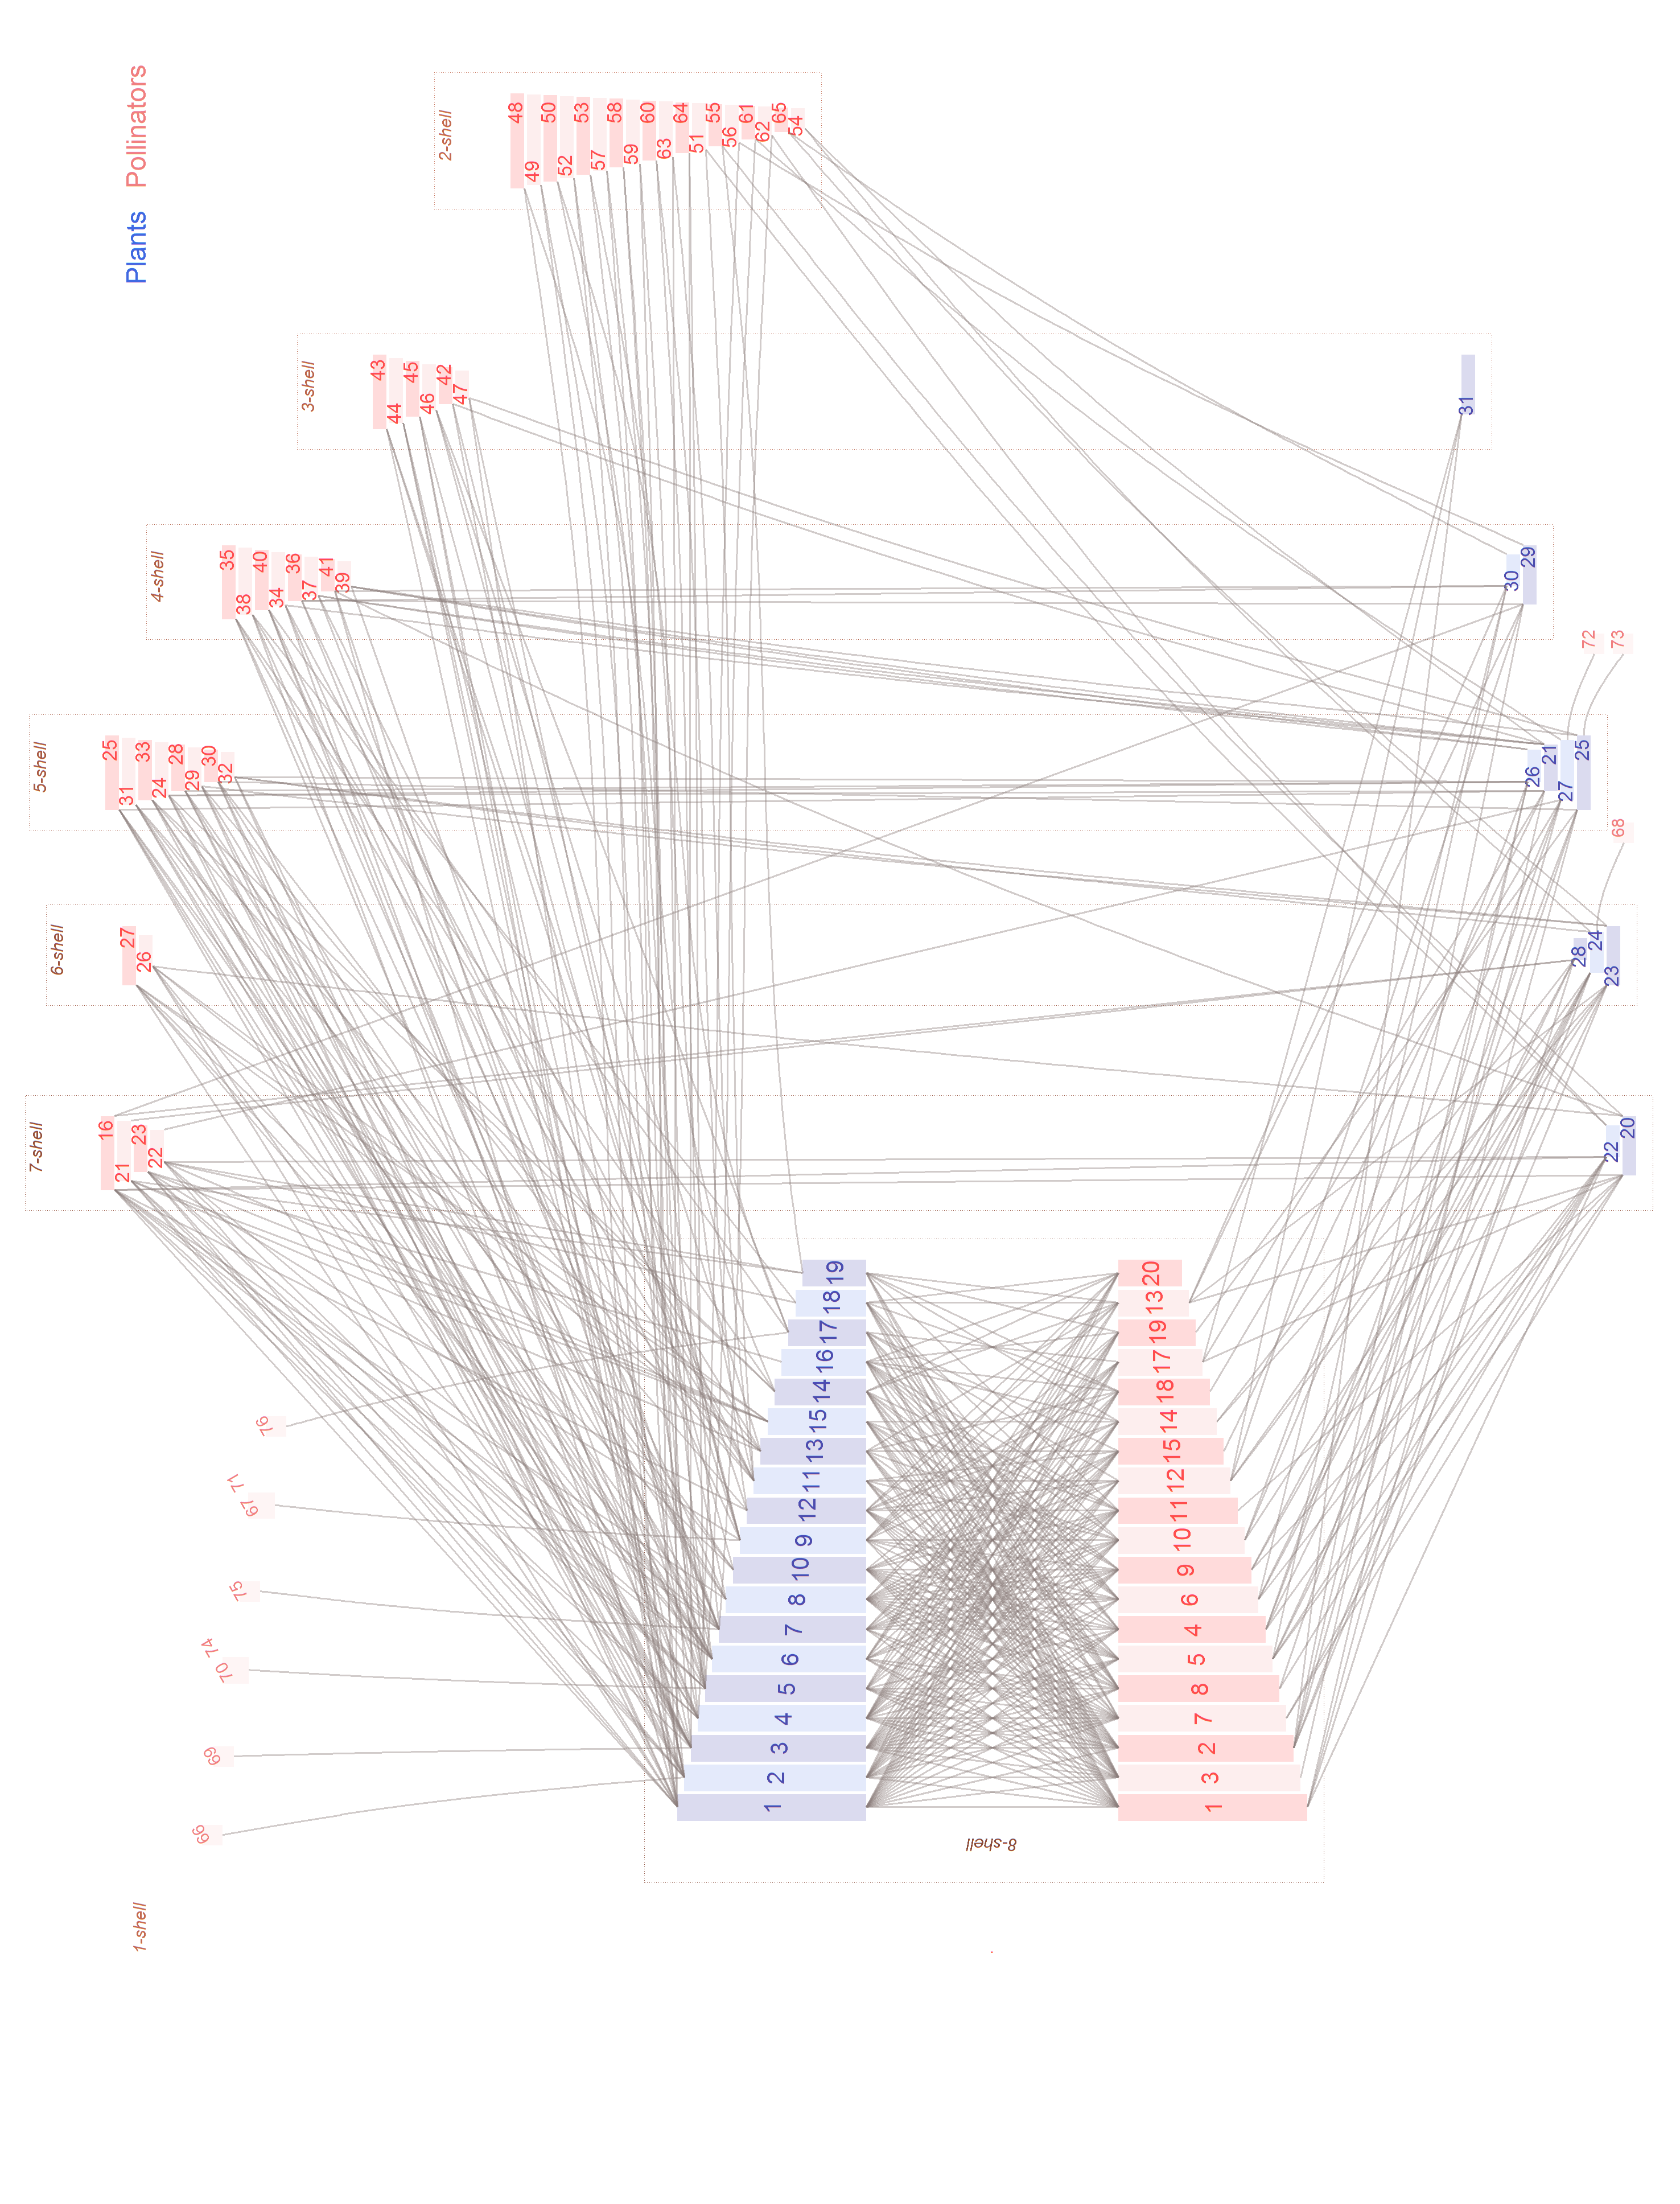
\includegraphics[scale=0.6]{Figures/VIS_M_PL_010_ziggurat.png}
\caption {Red de polinizadores $M\_PL\_010$ (Elberling \& Olesen, no publicada), con $107$ especies y $456$ enlaces. Su diagrama polar puede verse en la figura \ref{fig:VIS_Modvskdegree3}.}
\label{fig:VIS_M_PL_010_ziggurat}
\end{figure}

\clearpage
\begin{figure}[ht!]
\centering
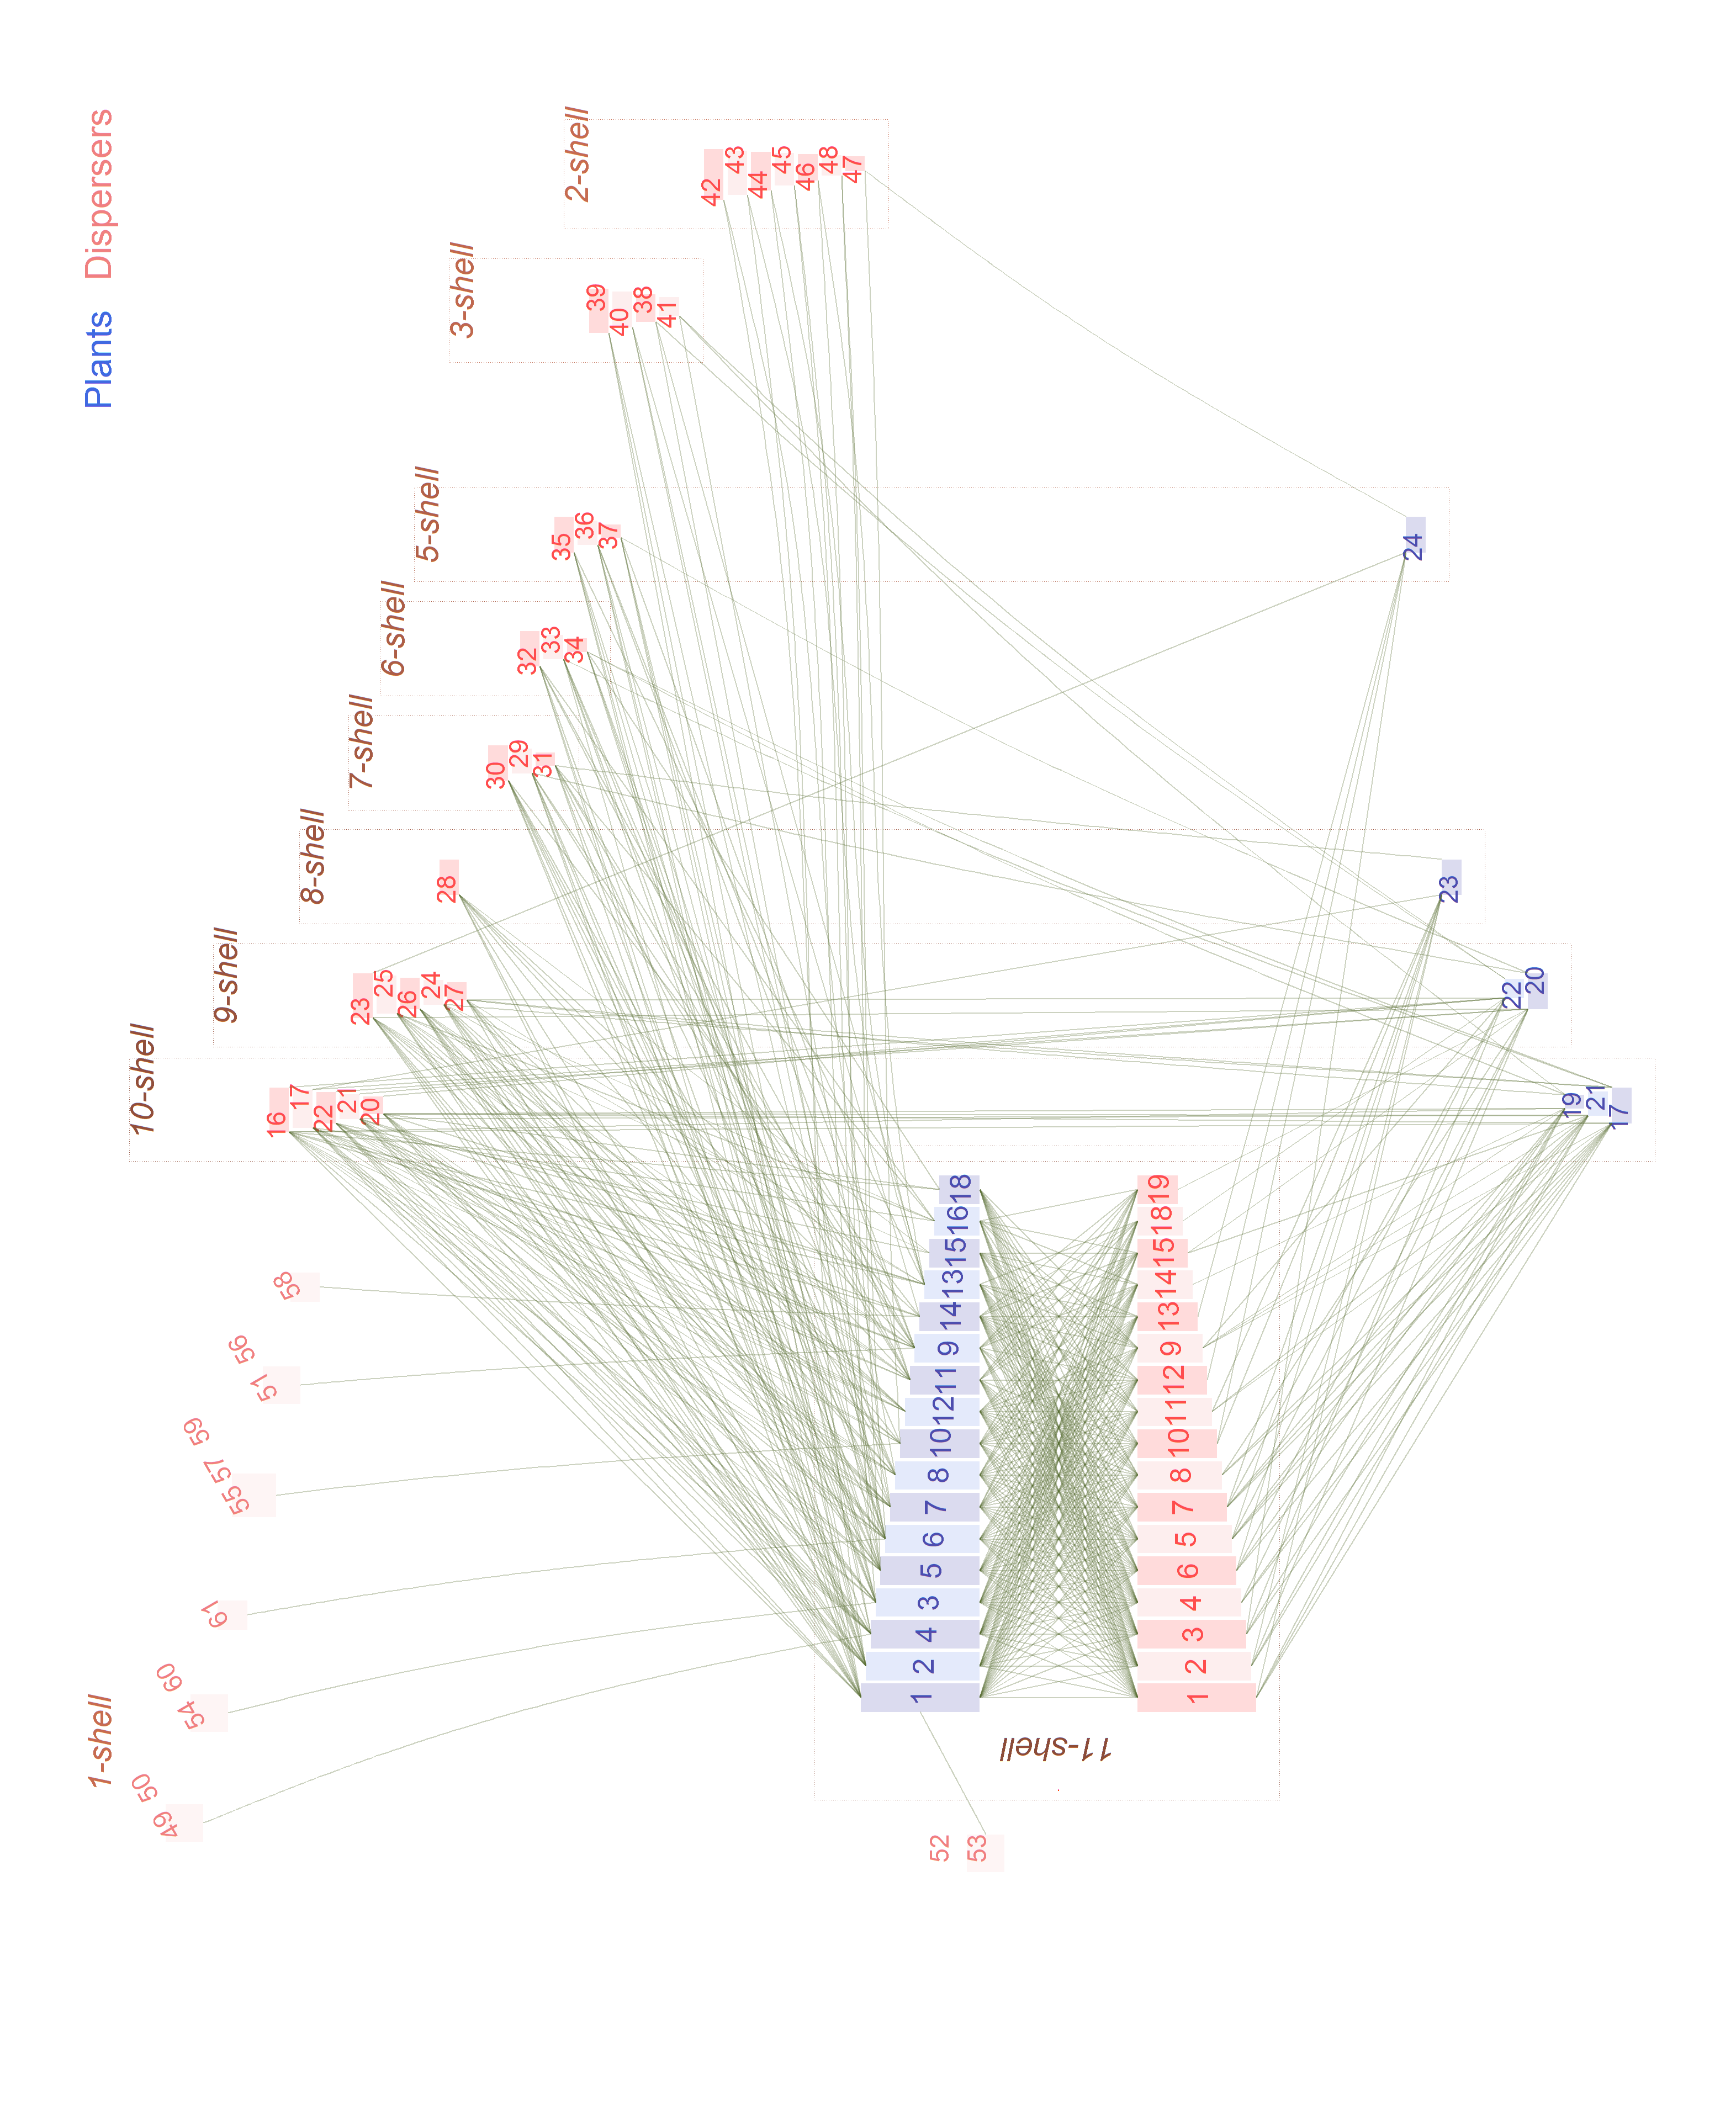
\includegraphics[scale=0.20]{Figures/VIS_M_SD_016_ziggurat.png}
\caption {Red de aves frugívoras $M\_SD\_016$ en la selva Kuala Lompat, Reserva de Krau Game, Malasia \cite{lambert1989fig}, con $85$ especies y $500$ enlaces.}
\label{fig:VIS_M_PL_047_ziggurat}
\end{figure}

\clearpage
\begin{figure}[ht!]
\centering
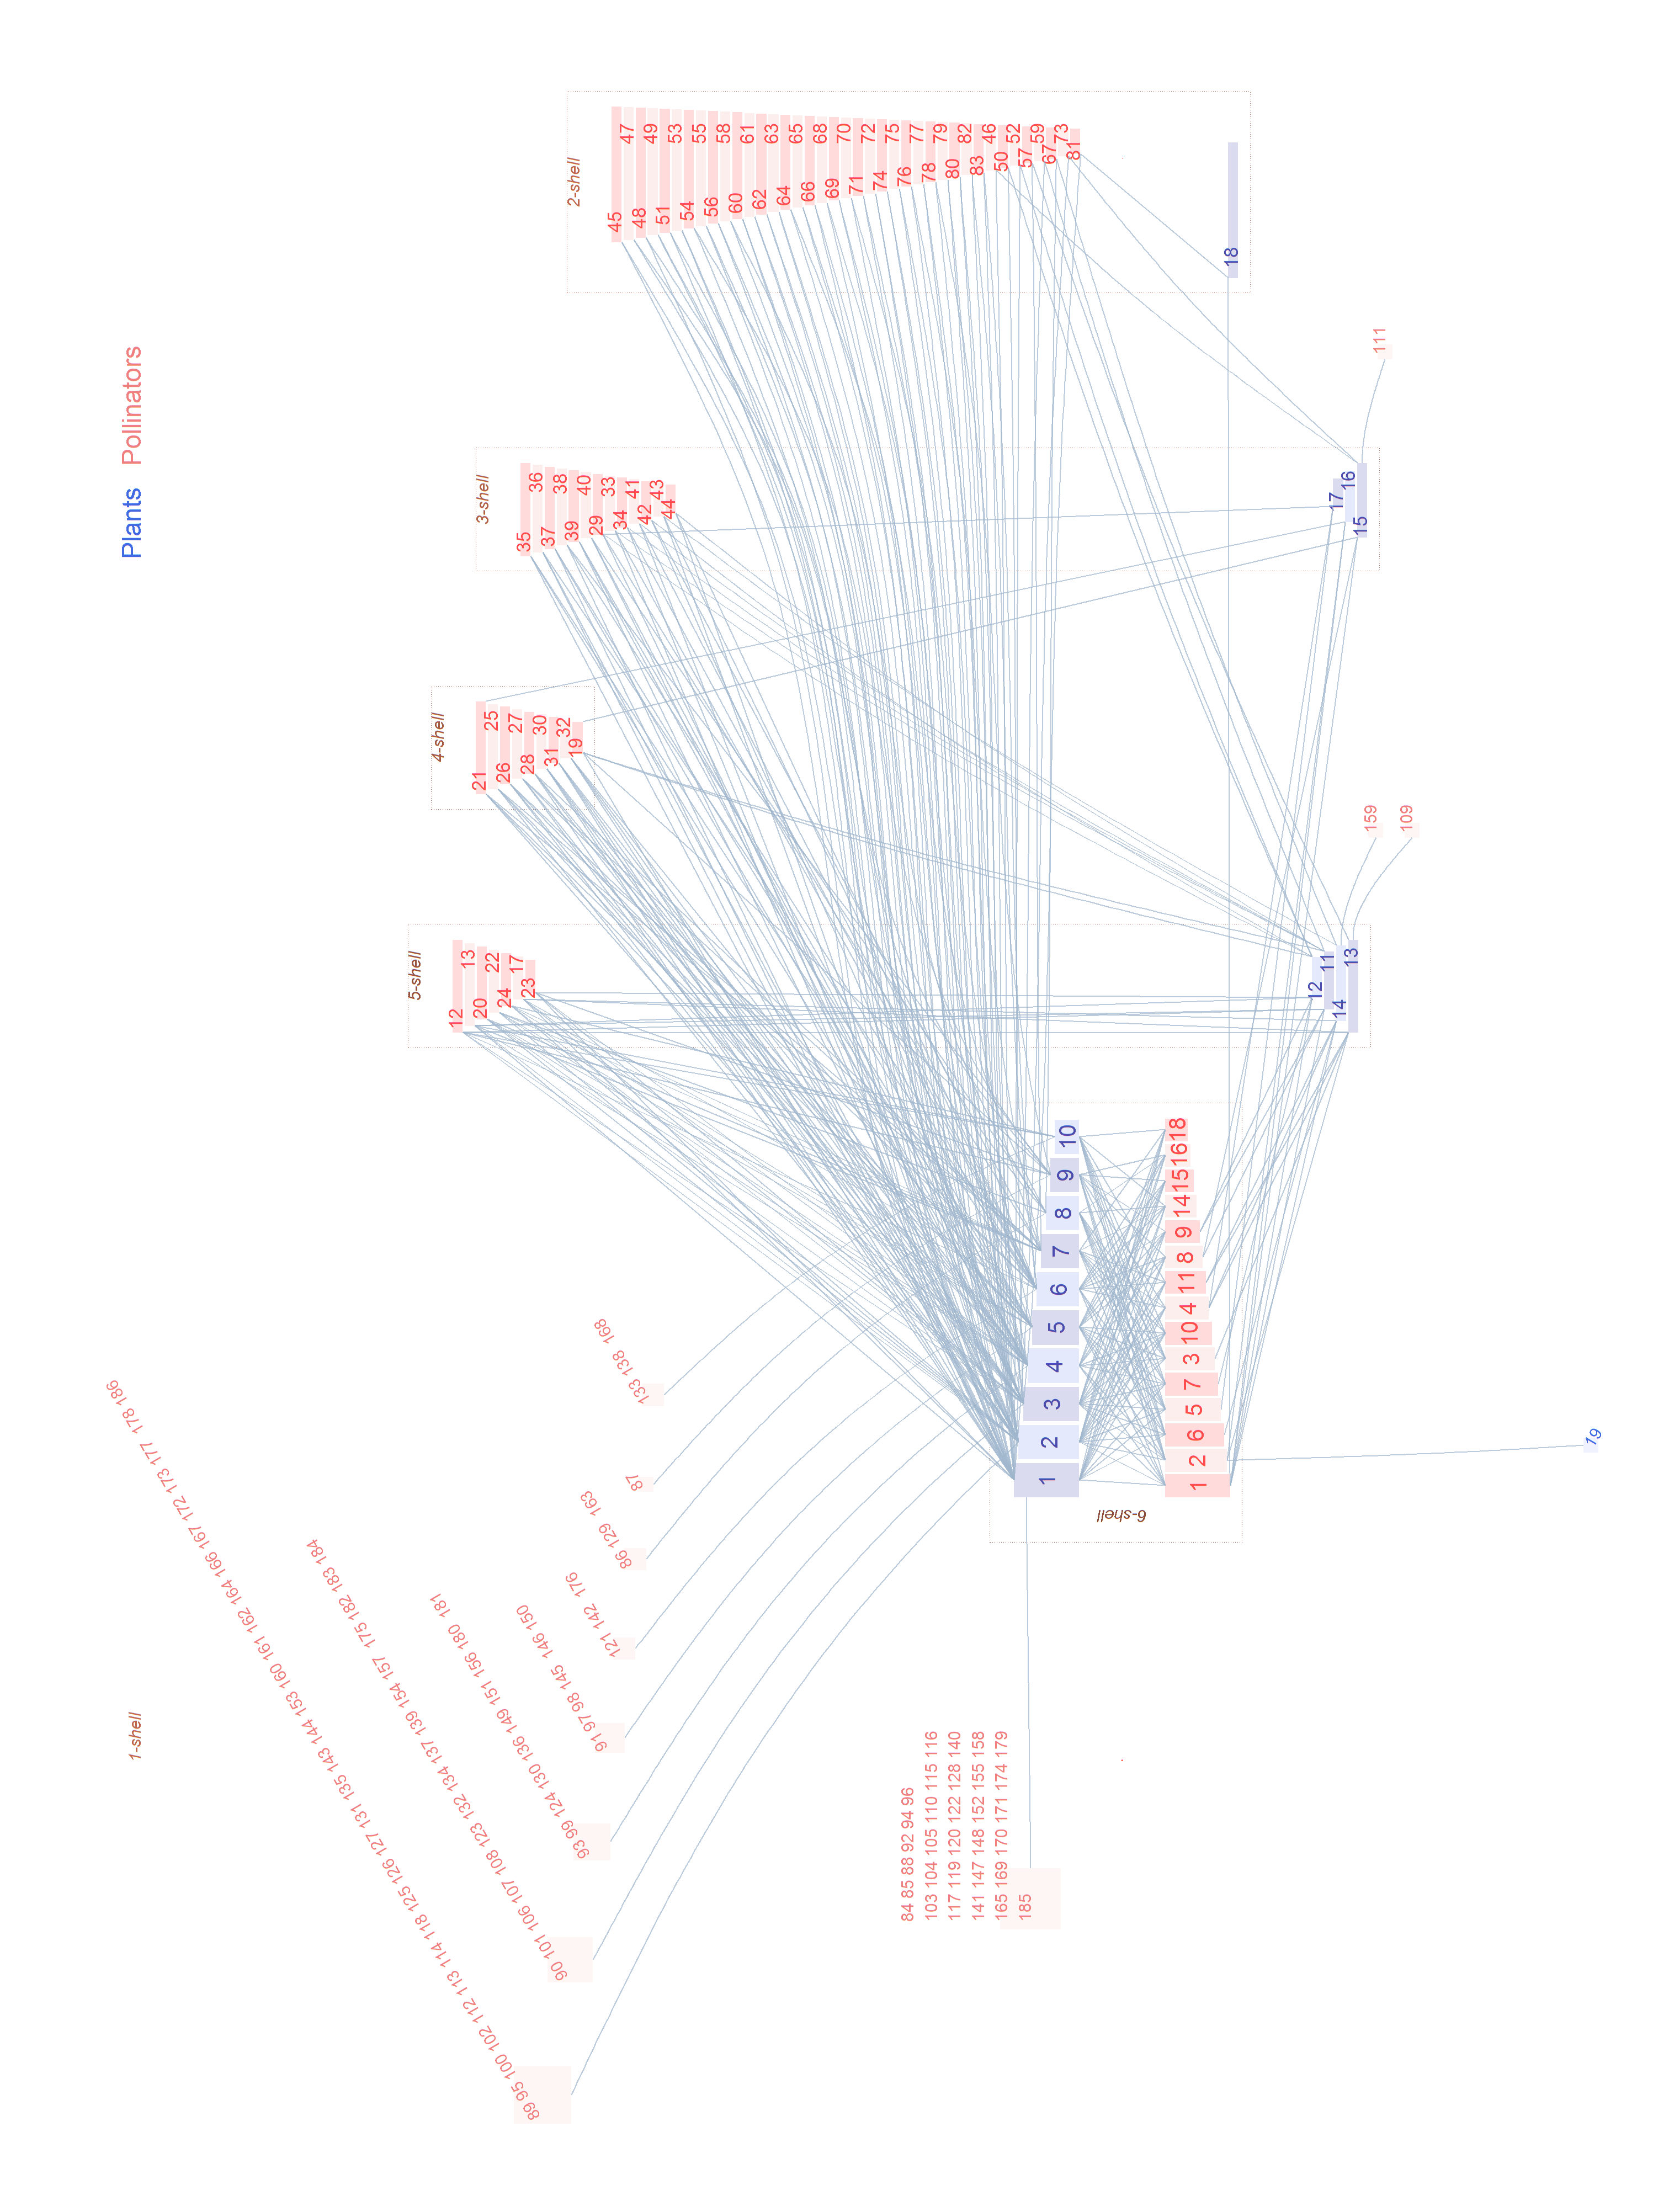
\includegraphics[scale=0.20]{Figures/VIS_M_PL_047_ziggurat.png}
\caption {Red de polinizadores $M\_PL\_047$, de un brezal en Isen Bjerg, Dinamarca \cite{dupont2009ecological}, con $205$ especies y $425$ enlaces.}
\label{fig:VIS_M_PL_047_ziggurat}
\end{figure}


\clearpage
\section{Visualización de la estructura}

El diagrama zigurat no solo sirve para captar la riqueza y variedad de las comunidades mutualistas, también puede ayudar a entender algunas de sus propiedades. En el capítulo anterior se describió un experimento que consiste en recablear al azar un pequeño porcentaje de los enlaces y medir su efecto en la correlación entre $NODF$ y $\overline k_{radius}$ (figura \ref{fig:ESTATICA_histo_corr_rewiring}). La mayoría de las redes experimentan una degradaciónl lineal por la que el anidamiento medido con $NODF$ decrece y el $\overline k_{radius}$ aumenta. Se llega a un estado similar al que se obtendría si las especies interactuasen al azar, lo que sabemos que está muy lejos de la realidad.

No obstante, un pequeño porcentaje se salía de este patrón. En general, eran redes pequeñas o con una marcada asimetría. En los dos ejemplos que se incluyen a continuación, los diagramas zigurat permiten entender el por qué de este comportamiento.

El primero (figura \ref{fig:VIS_PL_012}) corresponde a una red de tamaño mediano, con una estructura compleja. La red original se representa con los colores habituales, las correspondientes a los distintos grados de recableado en otros tonos, para recalcar que no se trata de redes reales. 

En la red sin alterar, se observa un índice $k$ máximo de $4$, y una gran conectividad directa con esas \textit{shells}. Hay un importante número de especies en la $1$-$shell$. En el gráfico de correlación general entre $NODF$ y $\overline k_{radius}$ (figura \ref{fig:ESTATICA_corrfigs}) esta red se sitúa en una zona intermedia.

Cuando se reconectan al azar seis enlaces, la estructura cambia poco, aunque puede verse como aparece una $2$-$shell$ de plantas y aumenta la conectividad entre las \textit{k shells} inferiores. Es importante recalcar que esta red alterada es resultado de una realización aleatoria, la configuración puede variar entre distintos intentos, por eso las gráficas de la figura \ref{fig:ESTATICA_corrfigs} se obtuvieron repitiendo veinte veces el recabledado para un mismo número de enlaces. No obstante, un recableado mínimo como el del ejemplo, tiene pocas consecuencias para las medidas globales de esta red.

Al aumentar a diecisiete los enlaces reconectados, la degradación es más notable. El índice $k$ máximo baja a $3$. Si sigue creciendo la cantidad de reconexiones, la modificación es aun más evidente. En la imagen, para treinta y dos cambios al azar, las $2$-$shells$ han crecido a costa de la $3$ y aparecen muchas más conexiones, en proporción, entre ellas. La $NODF$ ha bajado desde el original $30,40$ a $12,22$ y el $\overline k_{radius}$ pasa de $2,51$ a $2,82$. 

En el segundo ejemplo se presenta un caso extremo de comportamiento fuera de la norma  (figura \ref{fig:VIS_SD_007}). Esta red de frugívoros es extraordinariamente asimétrica con solo $7$ especies de plantas por $72$ de animales. Las especies $1$ a $6$ de plantas forman la $3$-$shell$, solo la número $7$ tiene un lugar marginal en la $1$-$shell$.

\clearpage
\begin{figure}[ht!]
\centering
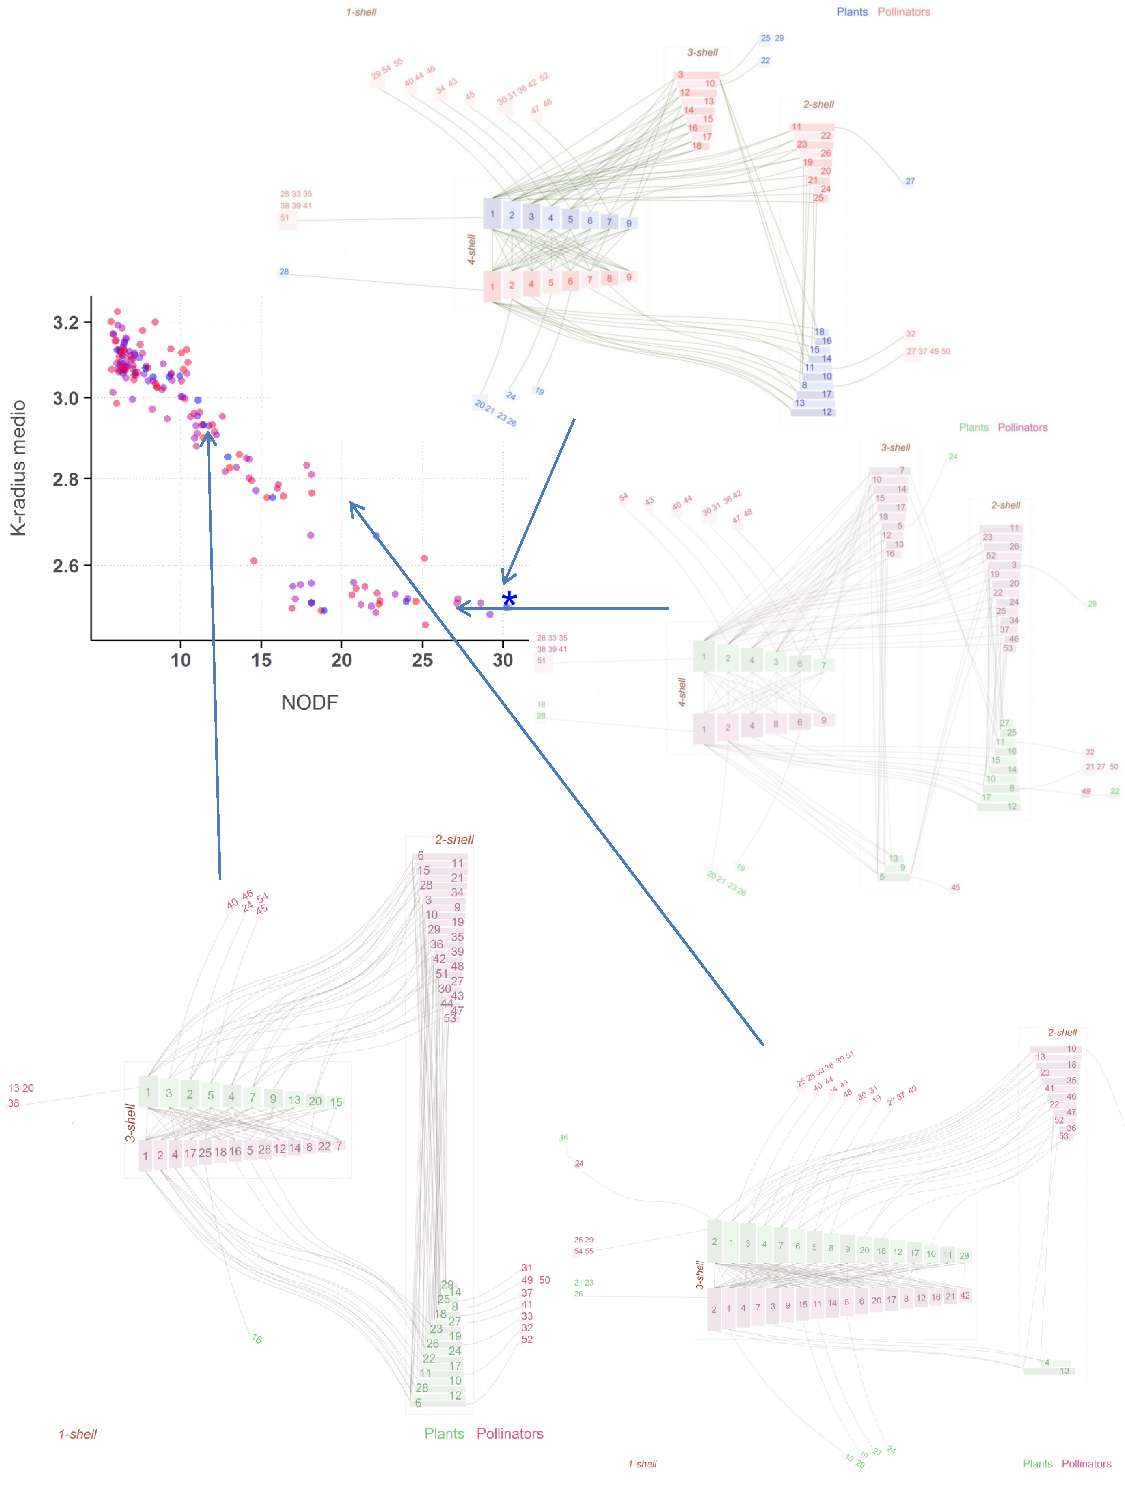
\includegraphics[scale=0.80]{Figures/VIS_PL_012.pdf}
\caption {Red de polinizadores $M\_PL\_012$, en el Parque Nacional de Garajonay, La Gomera (España), compilada por Olesen y no publicada, con $84$ especies y $145$ enlaces. Arriba, la red original, $NODF = 30,40$, $\overline k_{radius} = 2,51$. En sentido horario, red con siete enlaces recableados al azar, $NODF = 26,62$, $\overline k_{radius} = 2,48$; con diecisiete enlaces recableados, $NODF = 22,62$, $\overline k_{radius} = 2,77$ y con treinta y dos, $NODF = 13,22$, $\overline k_{radius} = 2,82$.}
\label{fig:VIS_PL_012}
\end{figure}

\clearpage
\begin{figure}[ht!]
\centering
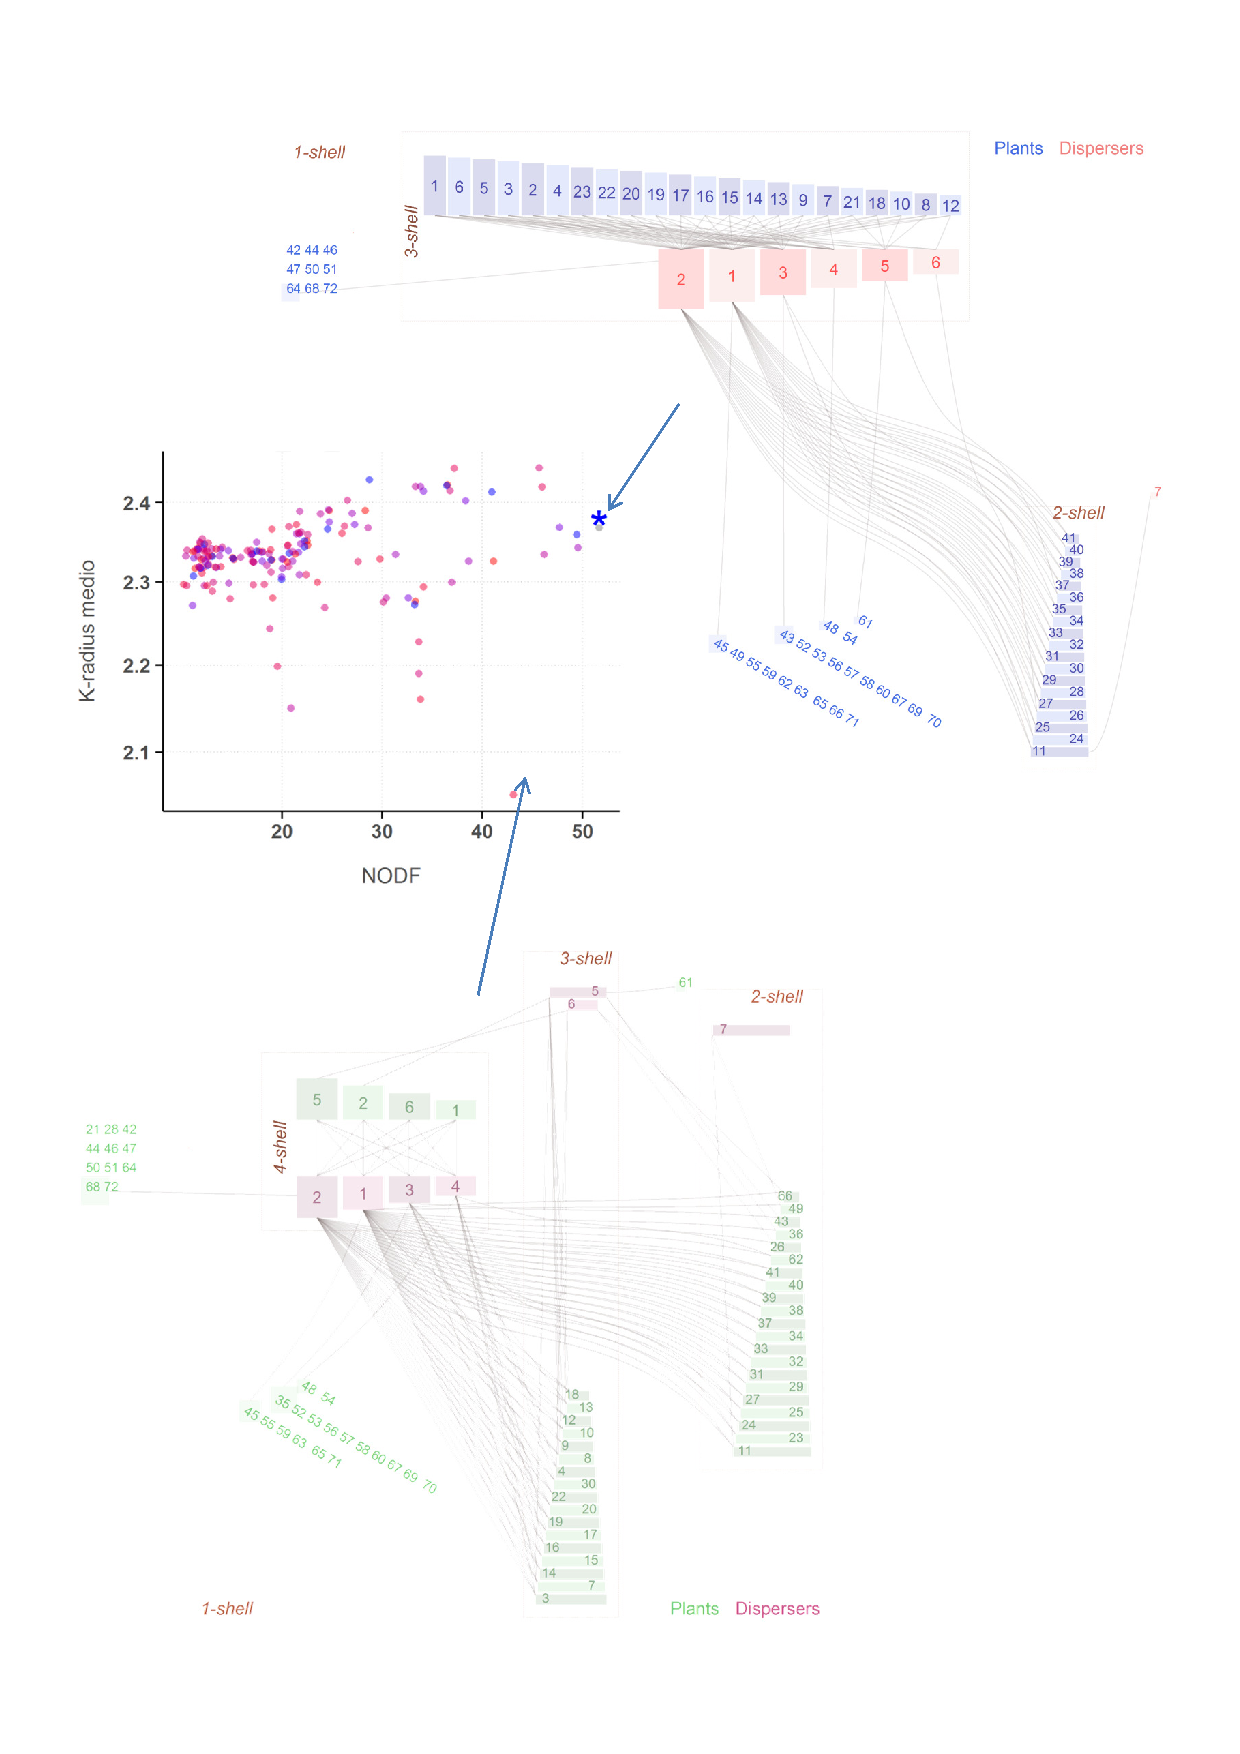
\includegraphics[scale=0.75]{Figures/VIS_SD_007.pdf}
\caption {Red de frugívoros $M\_SD\_007$, en el norte de Queensland, Australia \cite{crome1975ecology}, con $79$ especies y $143$ enlaces. Arriba, la red original, $NODF = 51,67$, $\overline k_{radius} = 2,37$. Abajo, red con seis enlaces recableados al azar, $NODF = 44,75$, $\overline k_{radius} = 2,09$.}
\label{fig:VIS_SD_007}
\end{figure}

\clearpage
Con esta configuración parece claro que una alteración mínima de las conexiones de las plantas tendrá un impacto sensible en la estructura global. Es lo que sucede recableando al azar solo seis enlaces. Aparece una $4$-$shell$ y disminuyen a la vez $NODF$ y  $\overline k_{radius}$. En el diagrama de correlación se ve que cualquier cambio disminuye el primer parámetro, pero esa información no dice nada sobre los profundos cambios de estructura que podrían producirse.

Una situación real en la que las redes cambian de forma drástica se produce por la extinción de una o más especies. En la figura \ref{fig:VIS_M_SD_004_pol3_pol4_ziggurat} se representa la red $M\_SD\_004$ (figura \ref{fig:ziggurat}), en la que se han eliminado únicamente los dos polinizadores de mayor $k_{degree}$, los números $3$ y $4$. El resultado es la reducción en $1$ del índice $k$ máximo, $NODF$ baja desde $39,82$ a $22,46$ y $\overline k_{radius}$ pasa de $2,19$ a $2,26$. La degradación de la red se asemeja a la que se ha visto con el experimento de recableado, con la fusión del $k$ máximo con el $k$-$1$ y el crecimiento de la proporción de enlaces entre especies fuera del $k$ máximo resultante.

\begin{figure}[ht!]
\centering
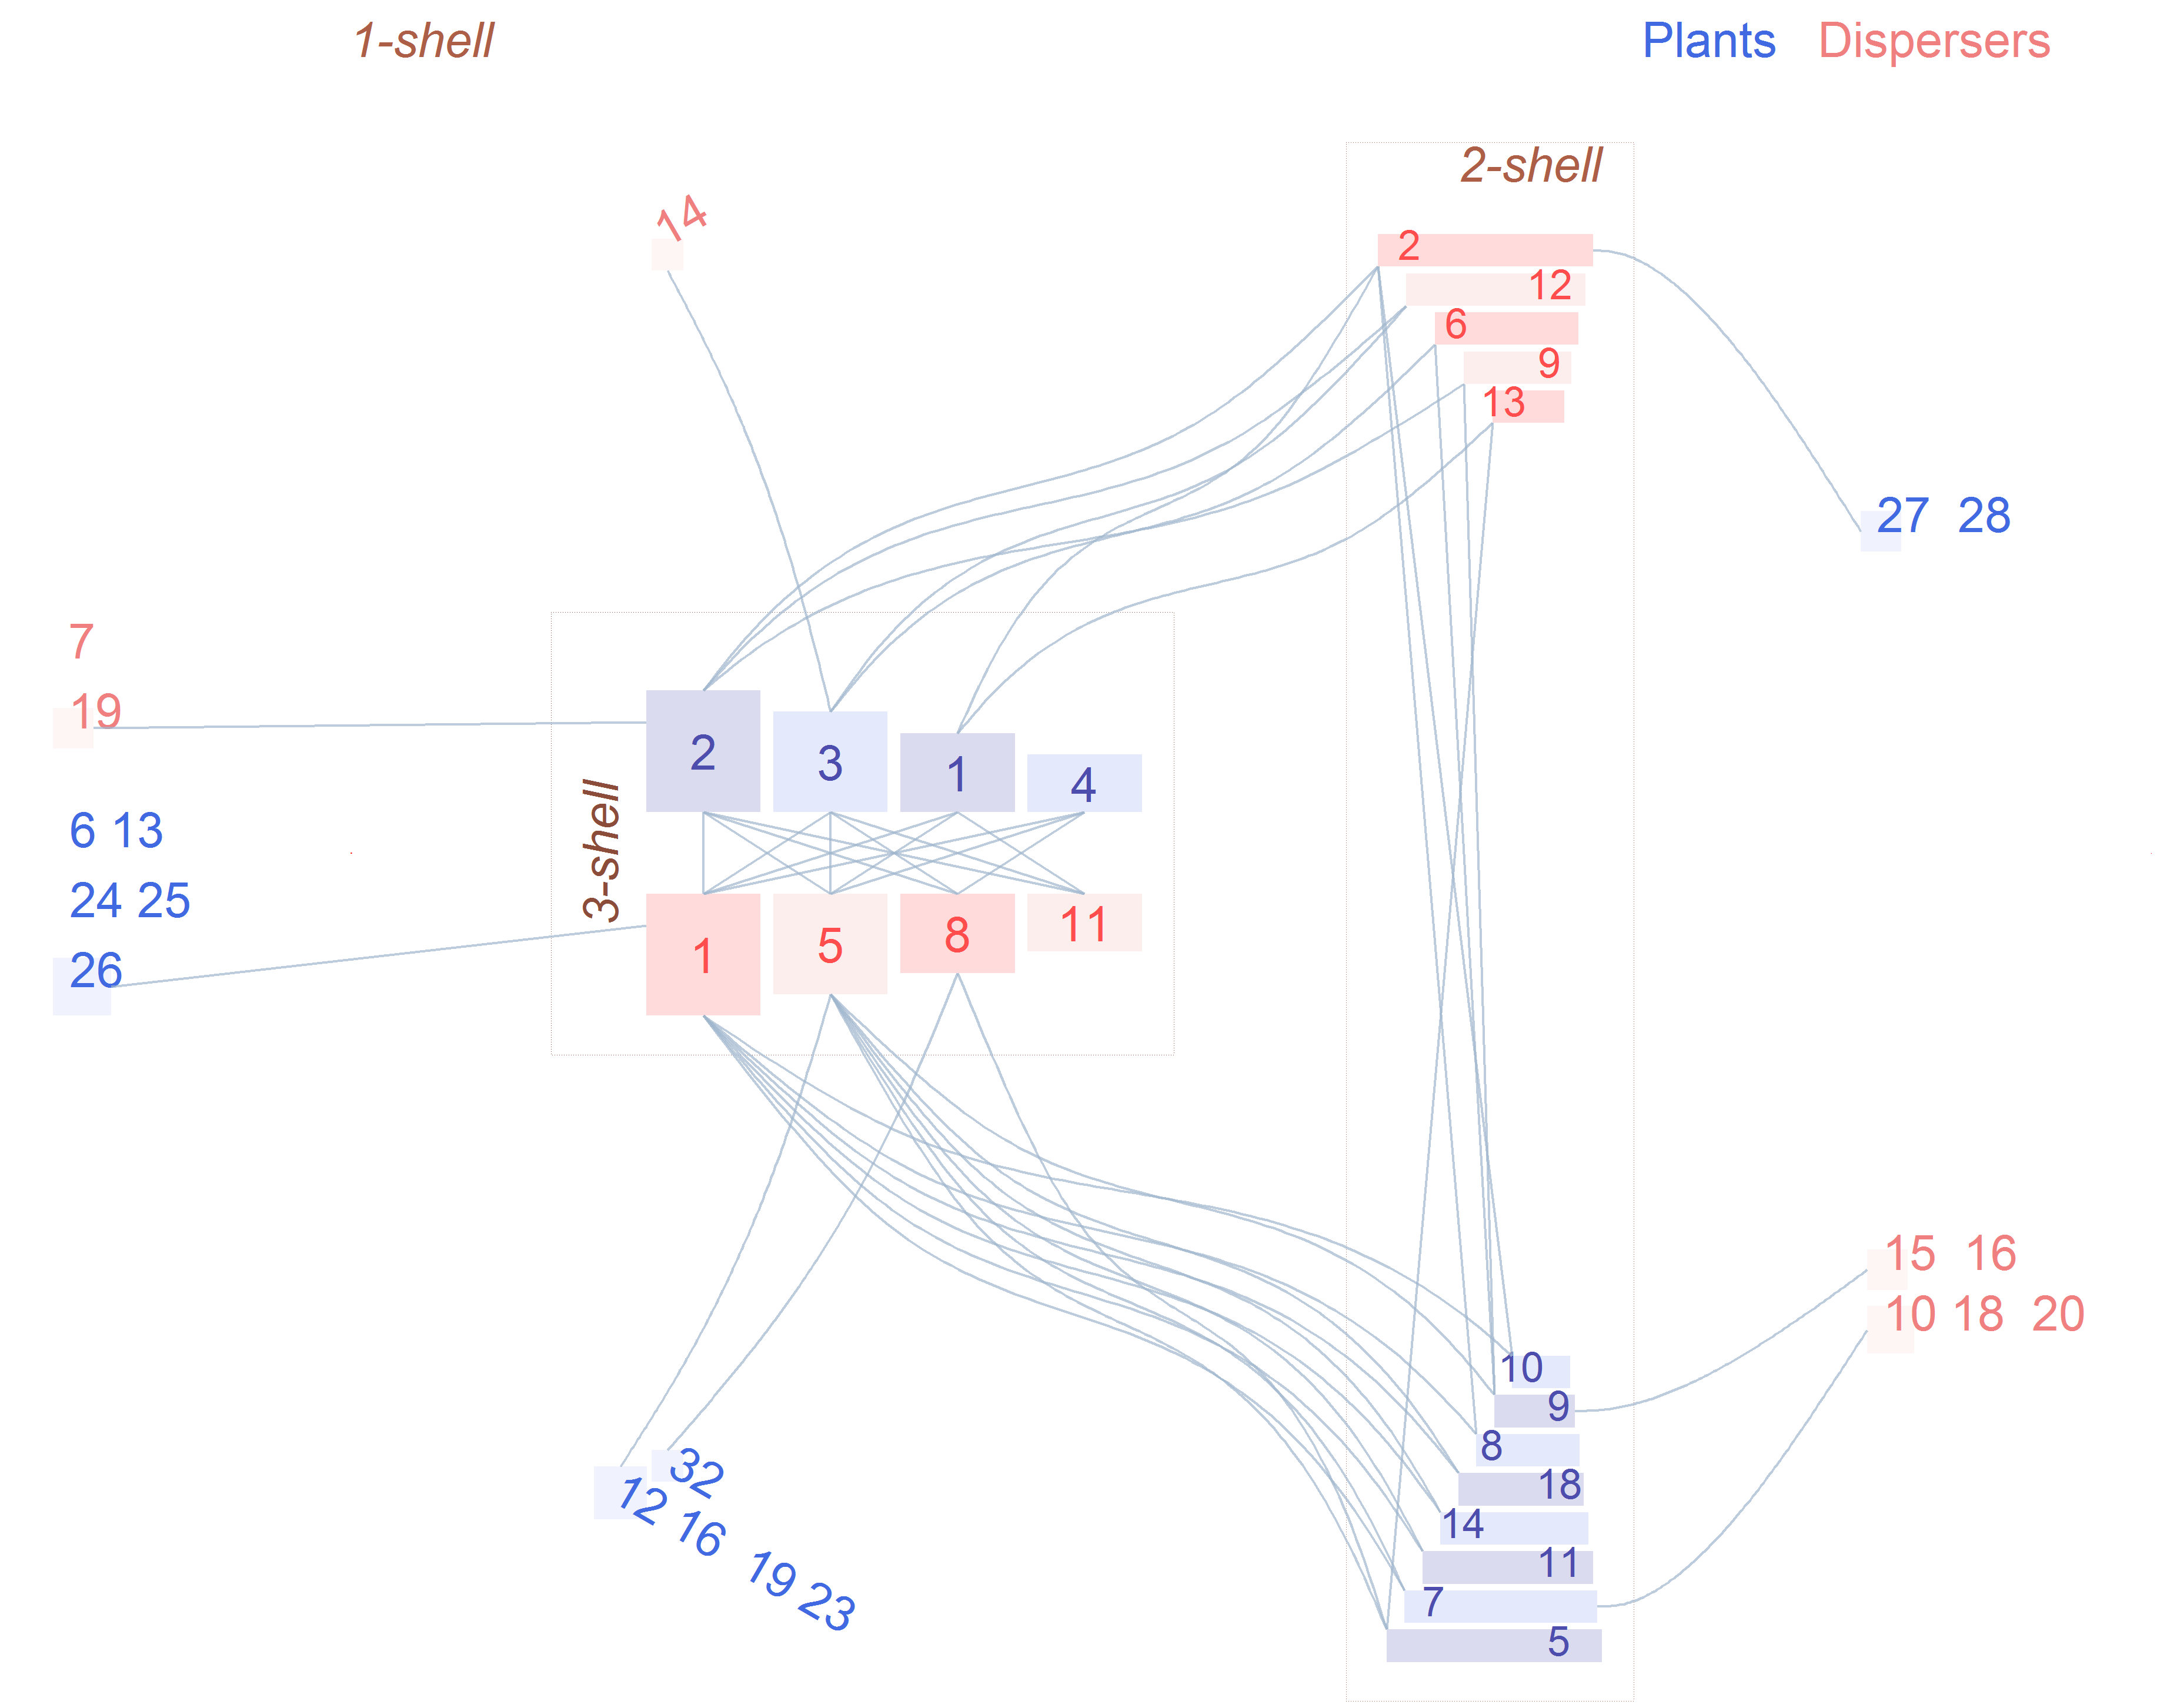
\includegraphics[scale=0.5]{Figures/VIS_M_SD_004_pol3_pol4_ziggurat.png}
\caption {Red de frugívoros $M\_SD\_004$, en la que se han eliminado los polinizadores números $3$ y $4$, los dos de mayor $k_{degree}$, véase la figura \ref{fig:ziggurat}.} 
\label{fig:VIS_M_SD_004_pol3_pol4_ziggurat}
\end{figure}

\clearpage
\begin{figure}[ht!]
\centering
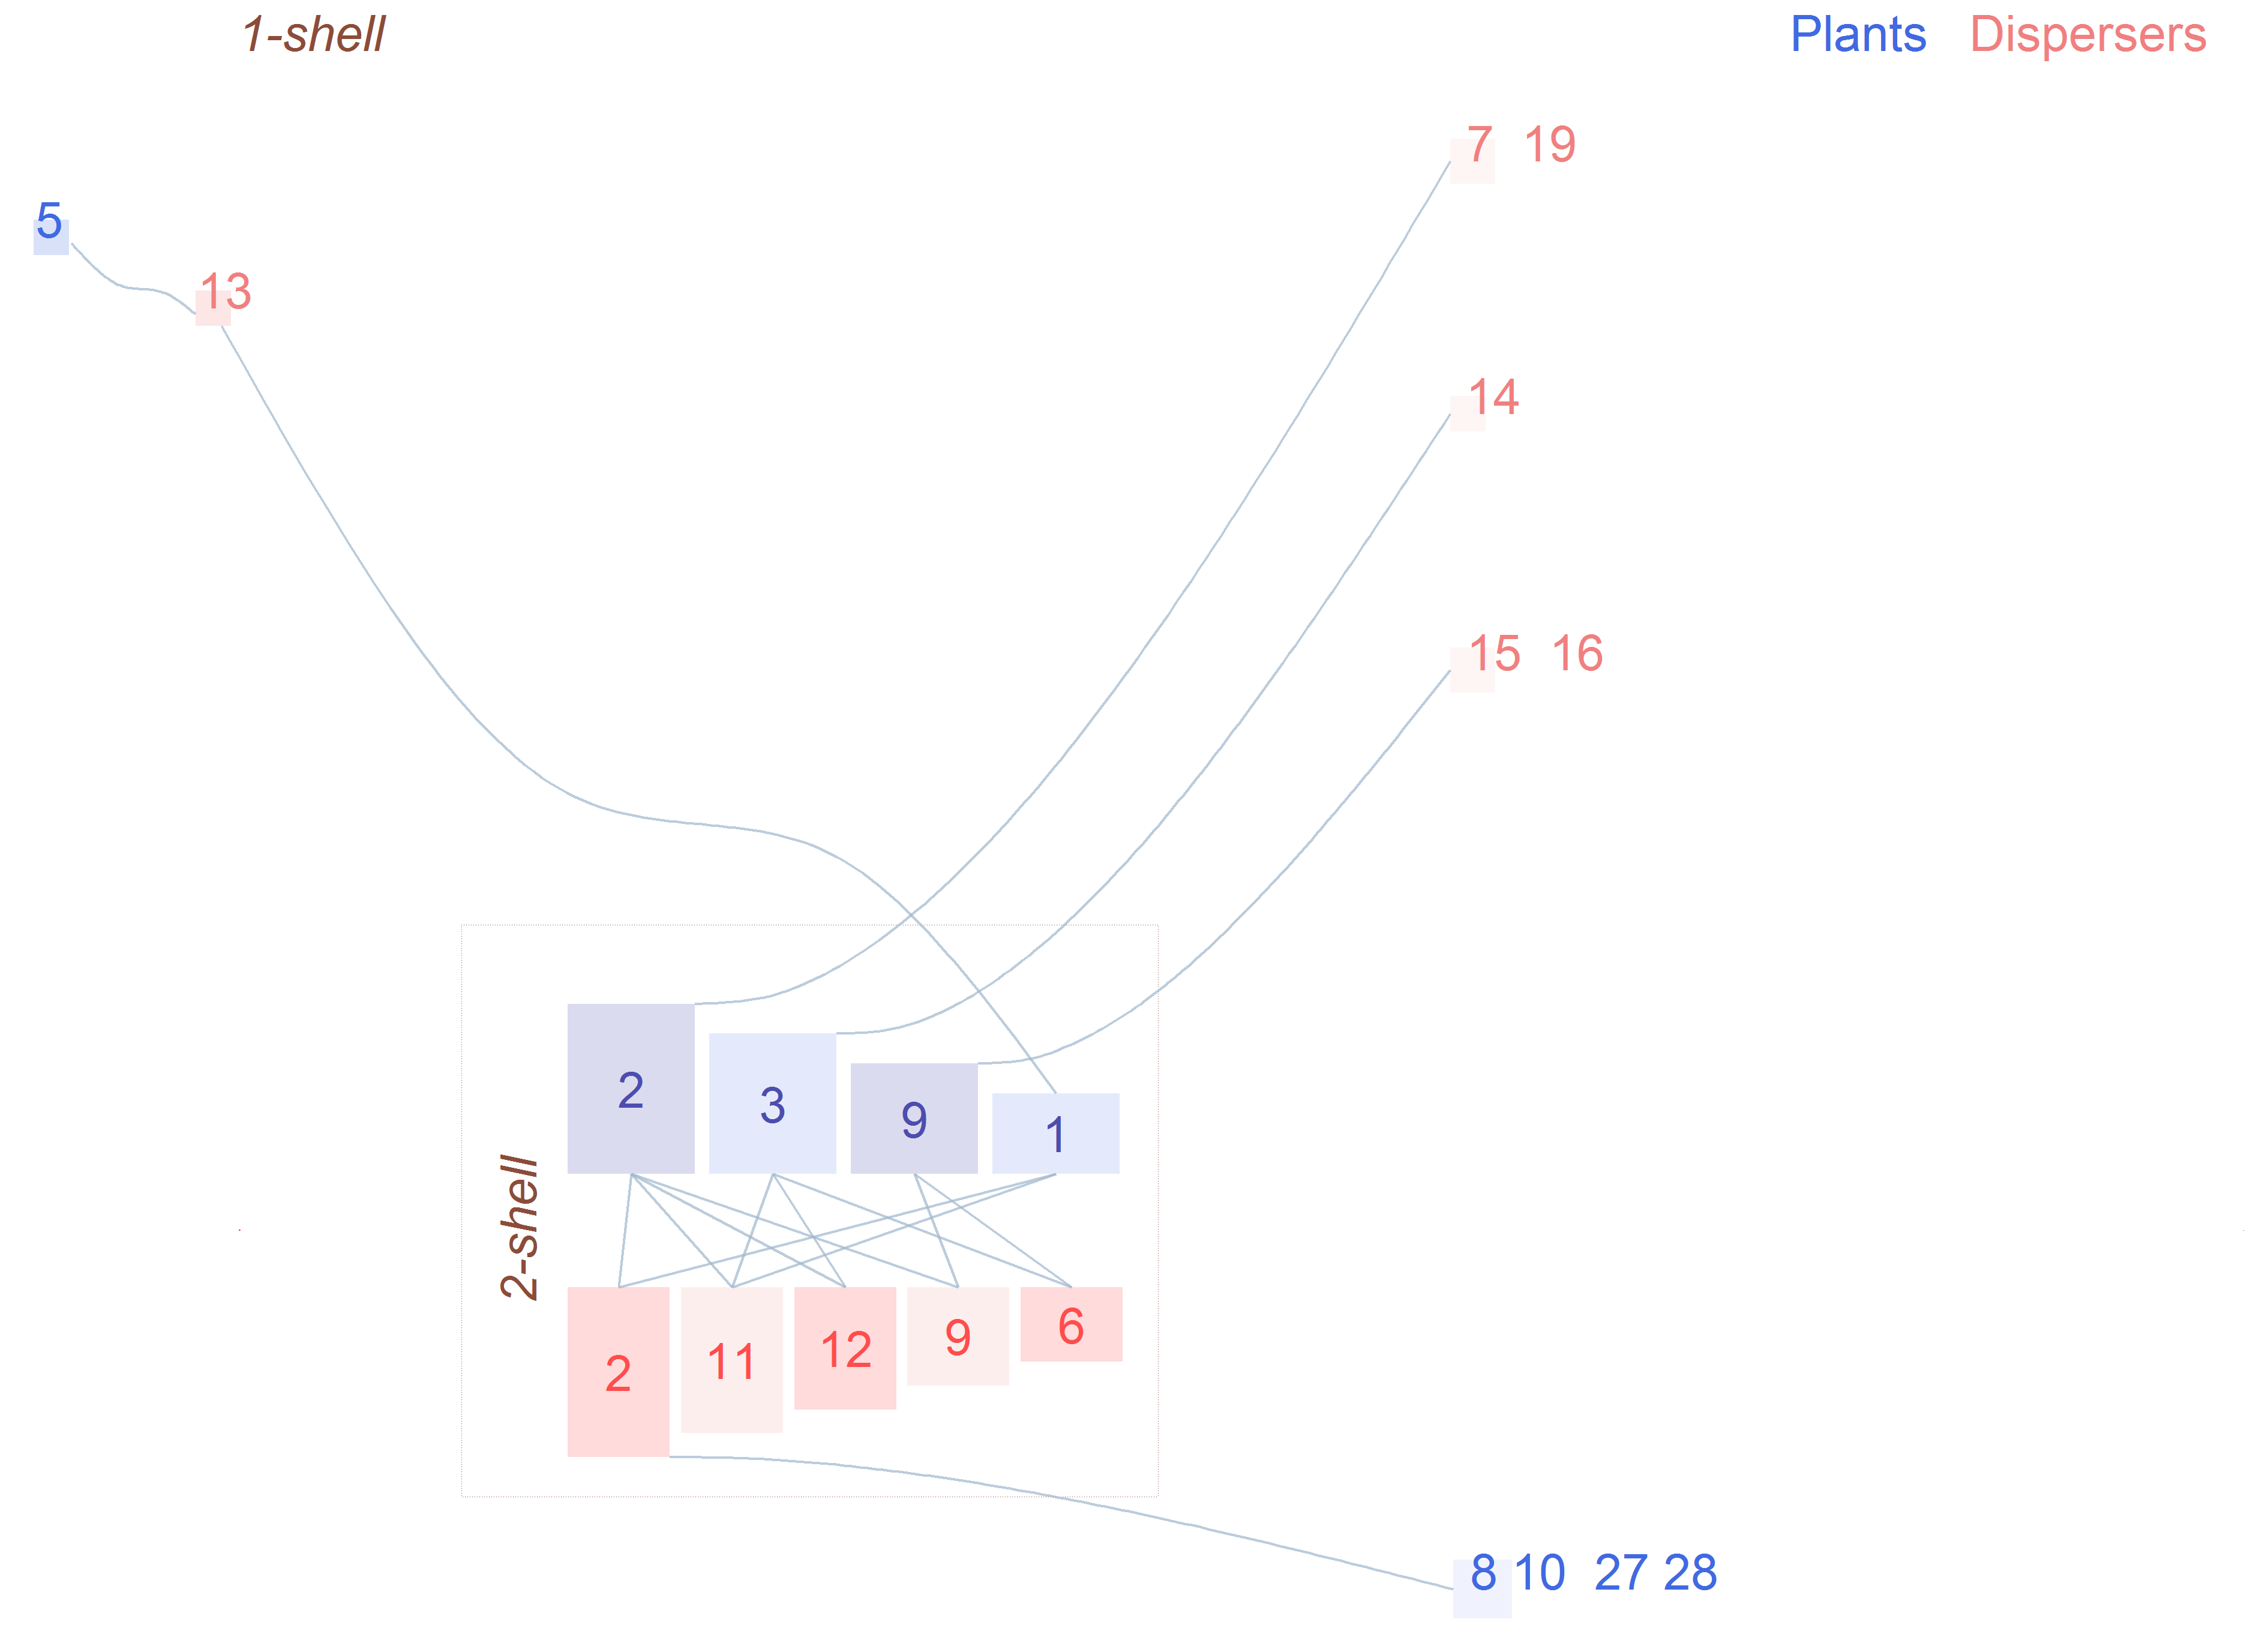
\includegraphics[scale=0.33]{Figures/VIS_M_SD_004_minus_k4_ziggurat.png}
\caption {Red de frugívoros $M\_SD\_004$, en la que se han eliminado todos los polinizadores de la $4$-$shell$, véase la figura \ref{fig:ziggurat}.} 
\label{fig:VIS_M_SD_004_minus_k4_ziggurat}
\end{figure}

\begin{figure}[h!]
\centering
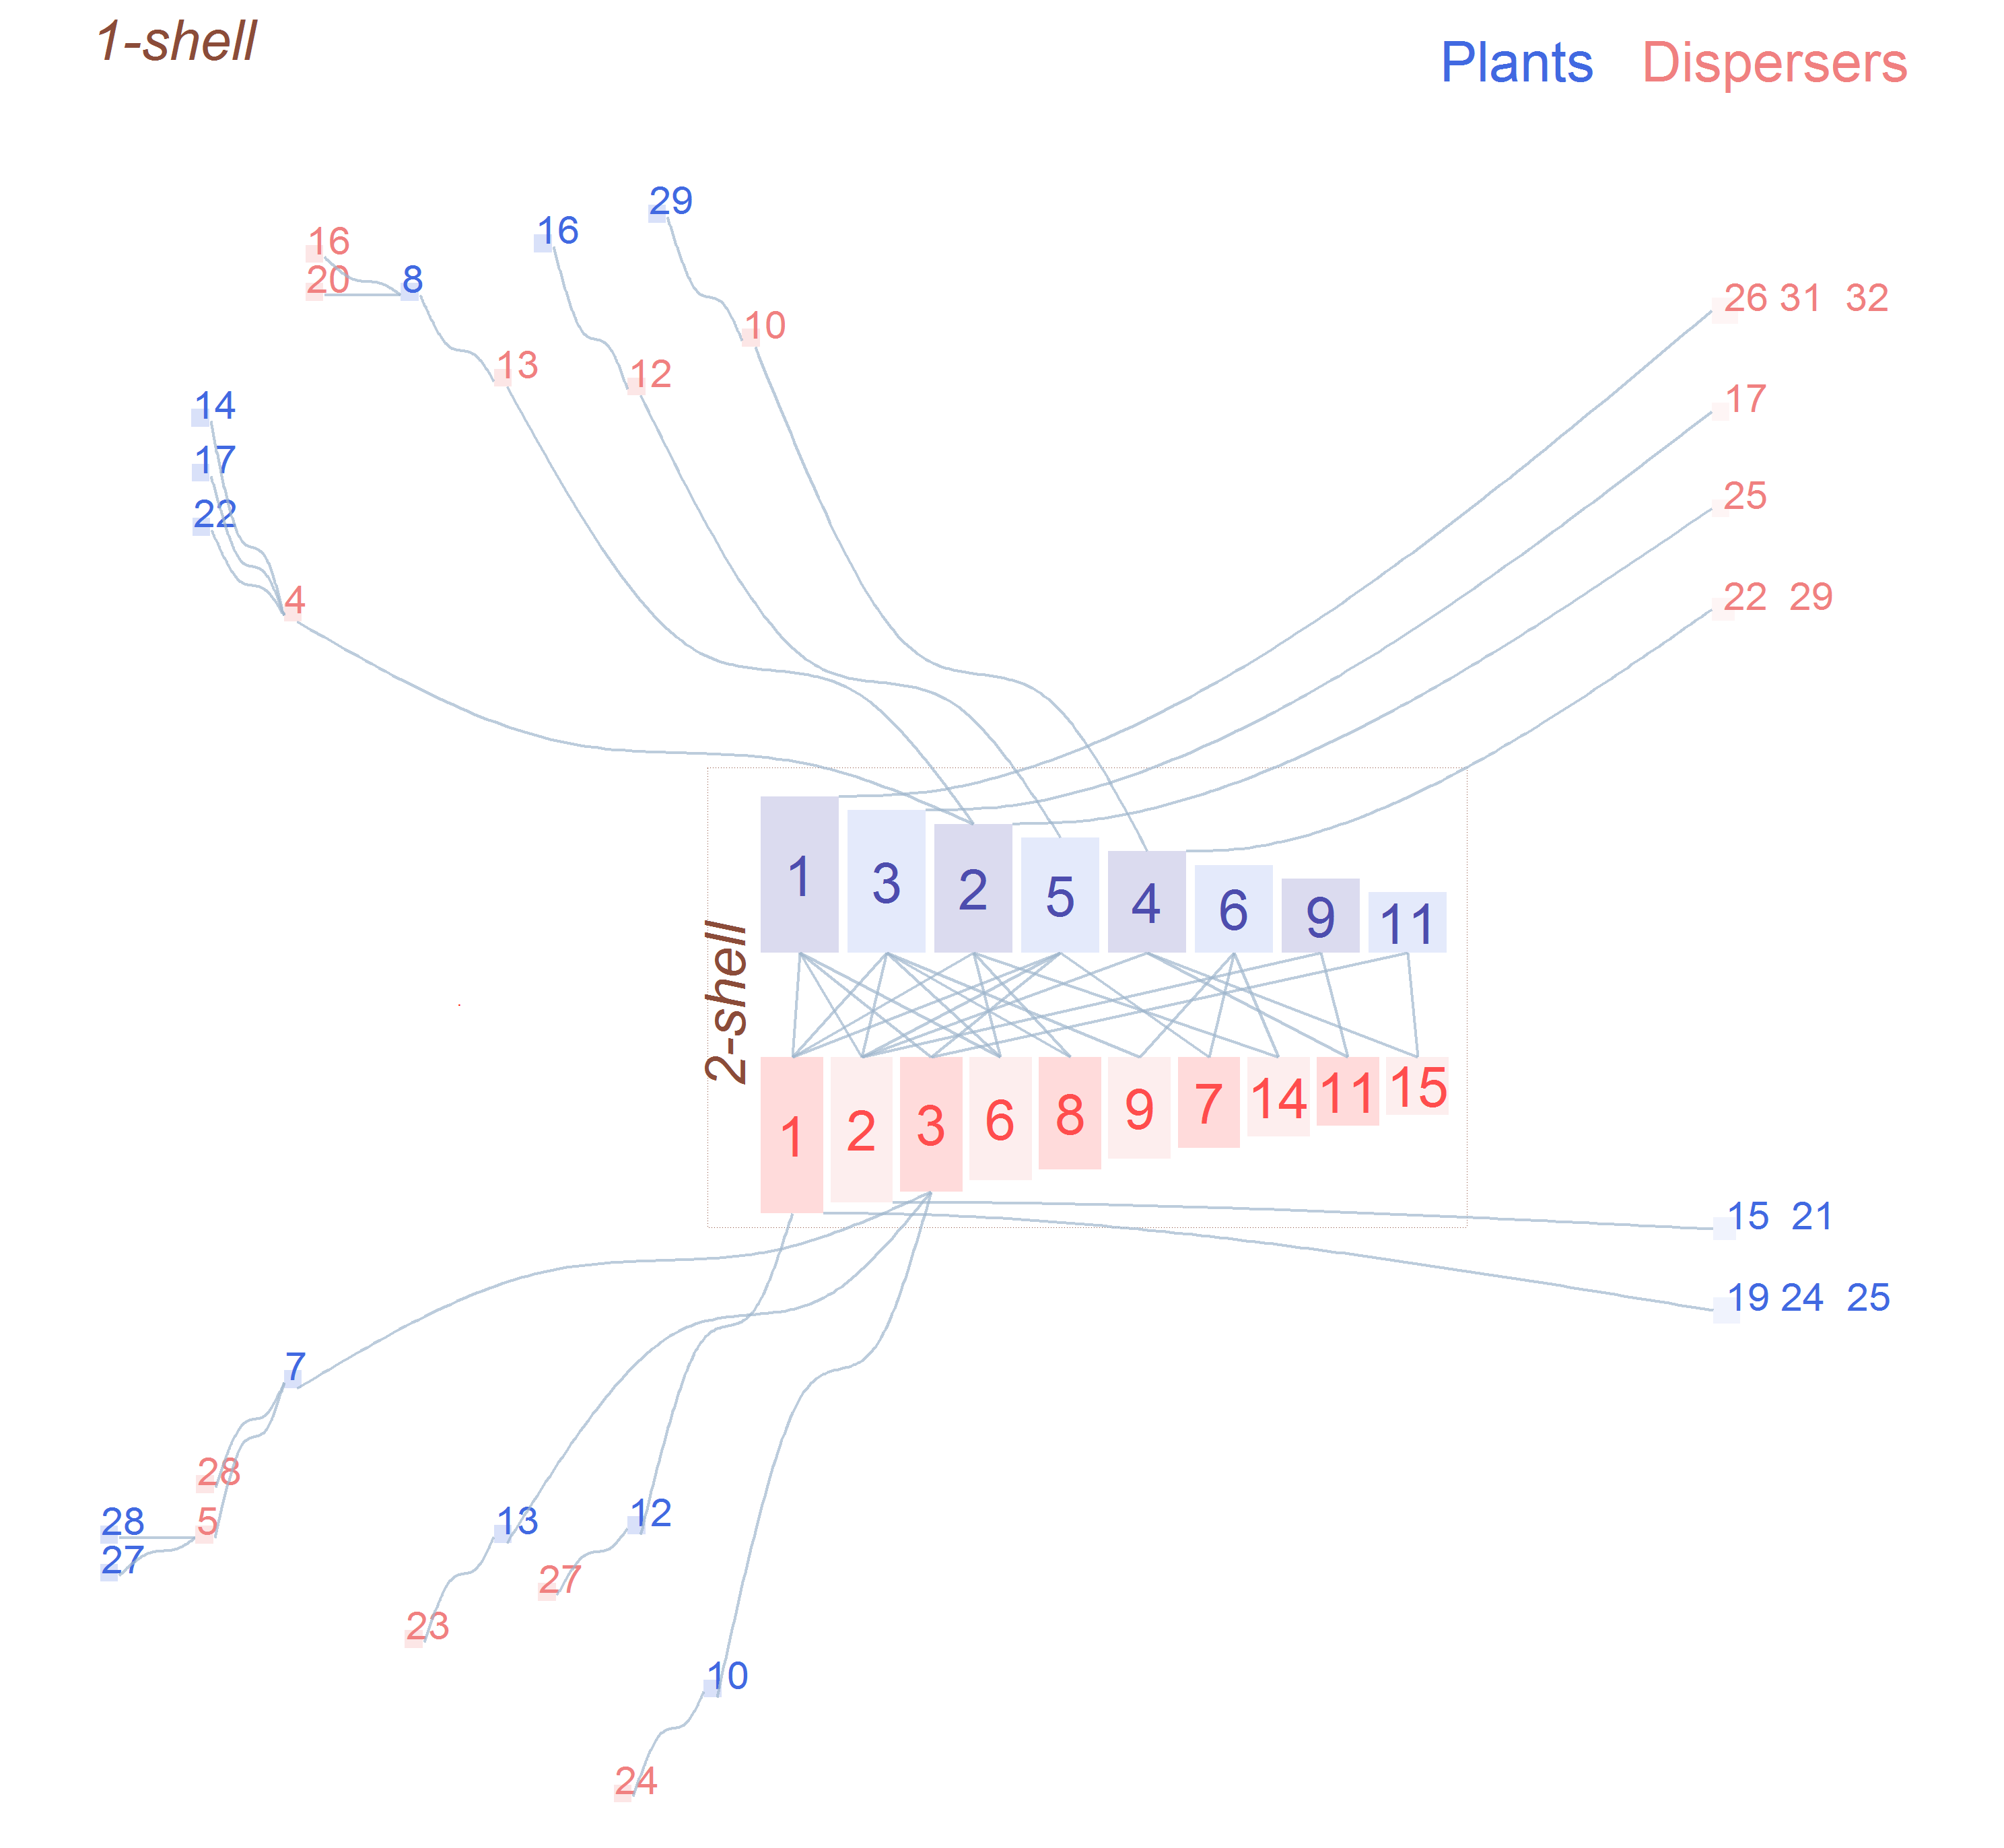
\includegraphics[scale=0.45]{Figures/VIS_M_SD_018_ziggurat.png}
\caption {Red de frugívoros $M\_SD\_018$, en Papúa Nueva Guinea \cite{mack1996notes}.} 
\label{fig:VIS_M_SD_018_ziggurat}
\end{figure}

El diagrama de zigurat permite ver de forma clara la importancia de la \textit{shell} máxima para la estabilidad de la red. Si desaparecen todas las especies de polinizadores de la $4$-$shell$ de manera simultánea ($1$,$3$,$4$,$5$ y $8$) el resultado es casi catastrófico para la comunidad. El anidamiento cae a $NODF = 3,38$. La red sobreviviente es un pequeño núcleo en $2$-$shell$ y escasas especies en $1$-$shell$ (figura \ref{fig:VIS_M_SD_004_minus_k4_ziggurat}).

En la figura \ref{fig:VIS_Modvskdegree3-sd04} se han representado los diagramas polares de la red intacta, de la red sin los dos polinizadores y de la red sin la $4$-$shell$ y el gráfico de la relación de $\overline k_{degree}$ con $Modularity$ como se hizo en la figura \ref{fig:VIS_Modvskdegree3-sd04}. Desde una posición inicial en la mitad del gráfico, los dos estados degradados se desplazan hacia posiciones de menor $k_{degree}$ y mayor $Modularity$.

\begin{figure}[h!]
\centering
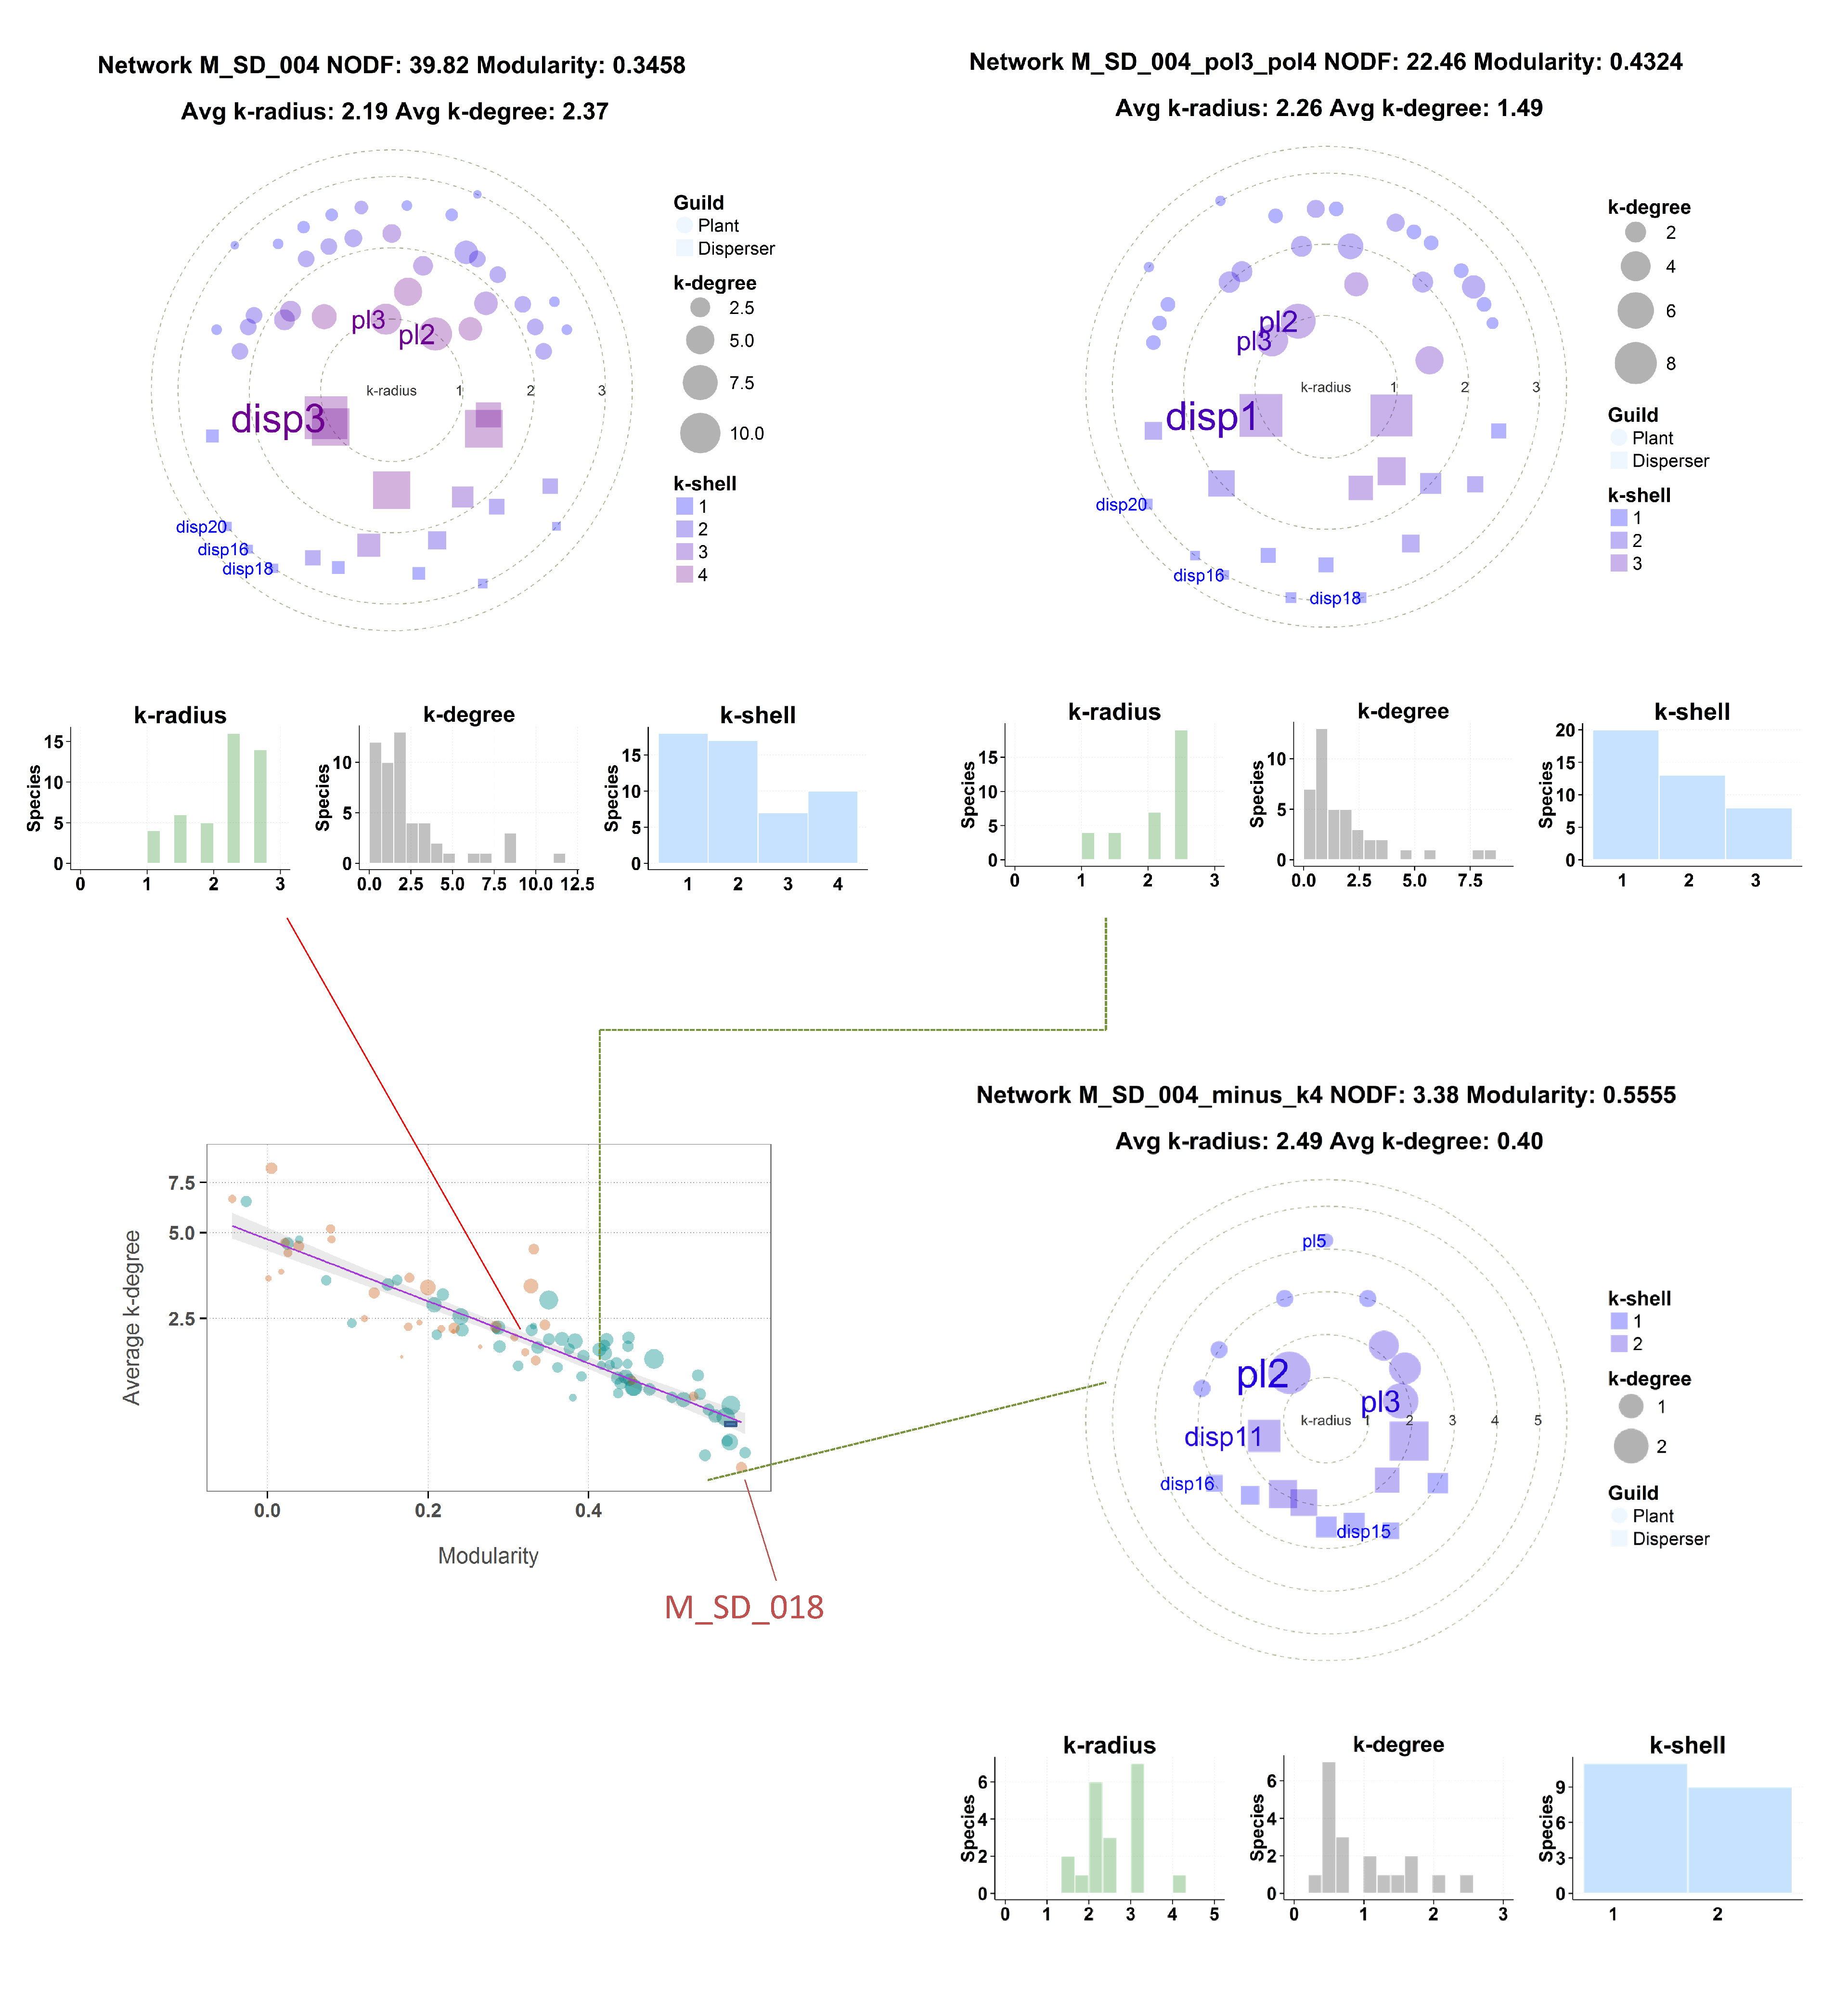
\includegraphics[scale=0.23]{Figures/VIS_Modvskdegree3-sd04.pdf}
\caption {Diagramas polares de la red $M\_SD\_004$ intacta, tras eliminar los dos polinizadores de mayor $k_{degree}$ y tras suprimir la $4$-$shell$ de polinizadores completa.} 
\label{fig:VIS_Modvskdegree3-sd04}
\end{figure}
 
\clearpage
\begin{figure}[ht!]
\centering
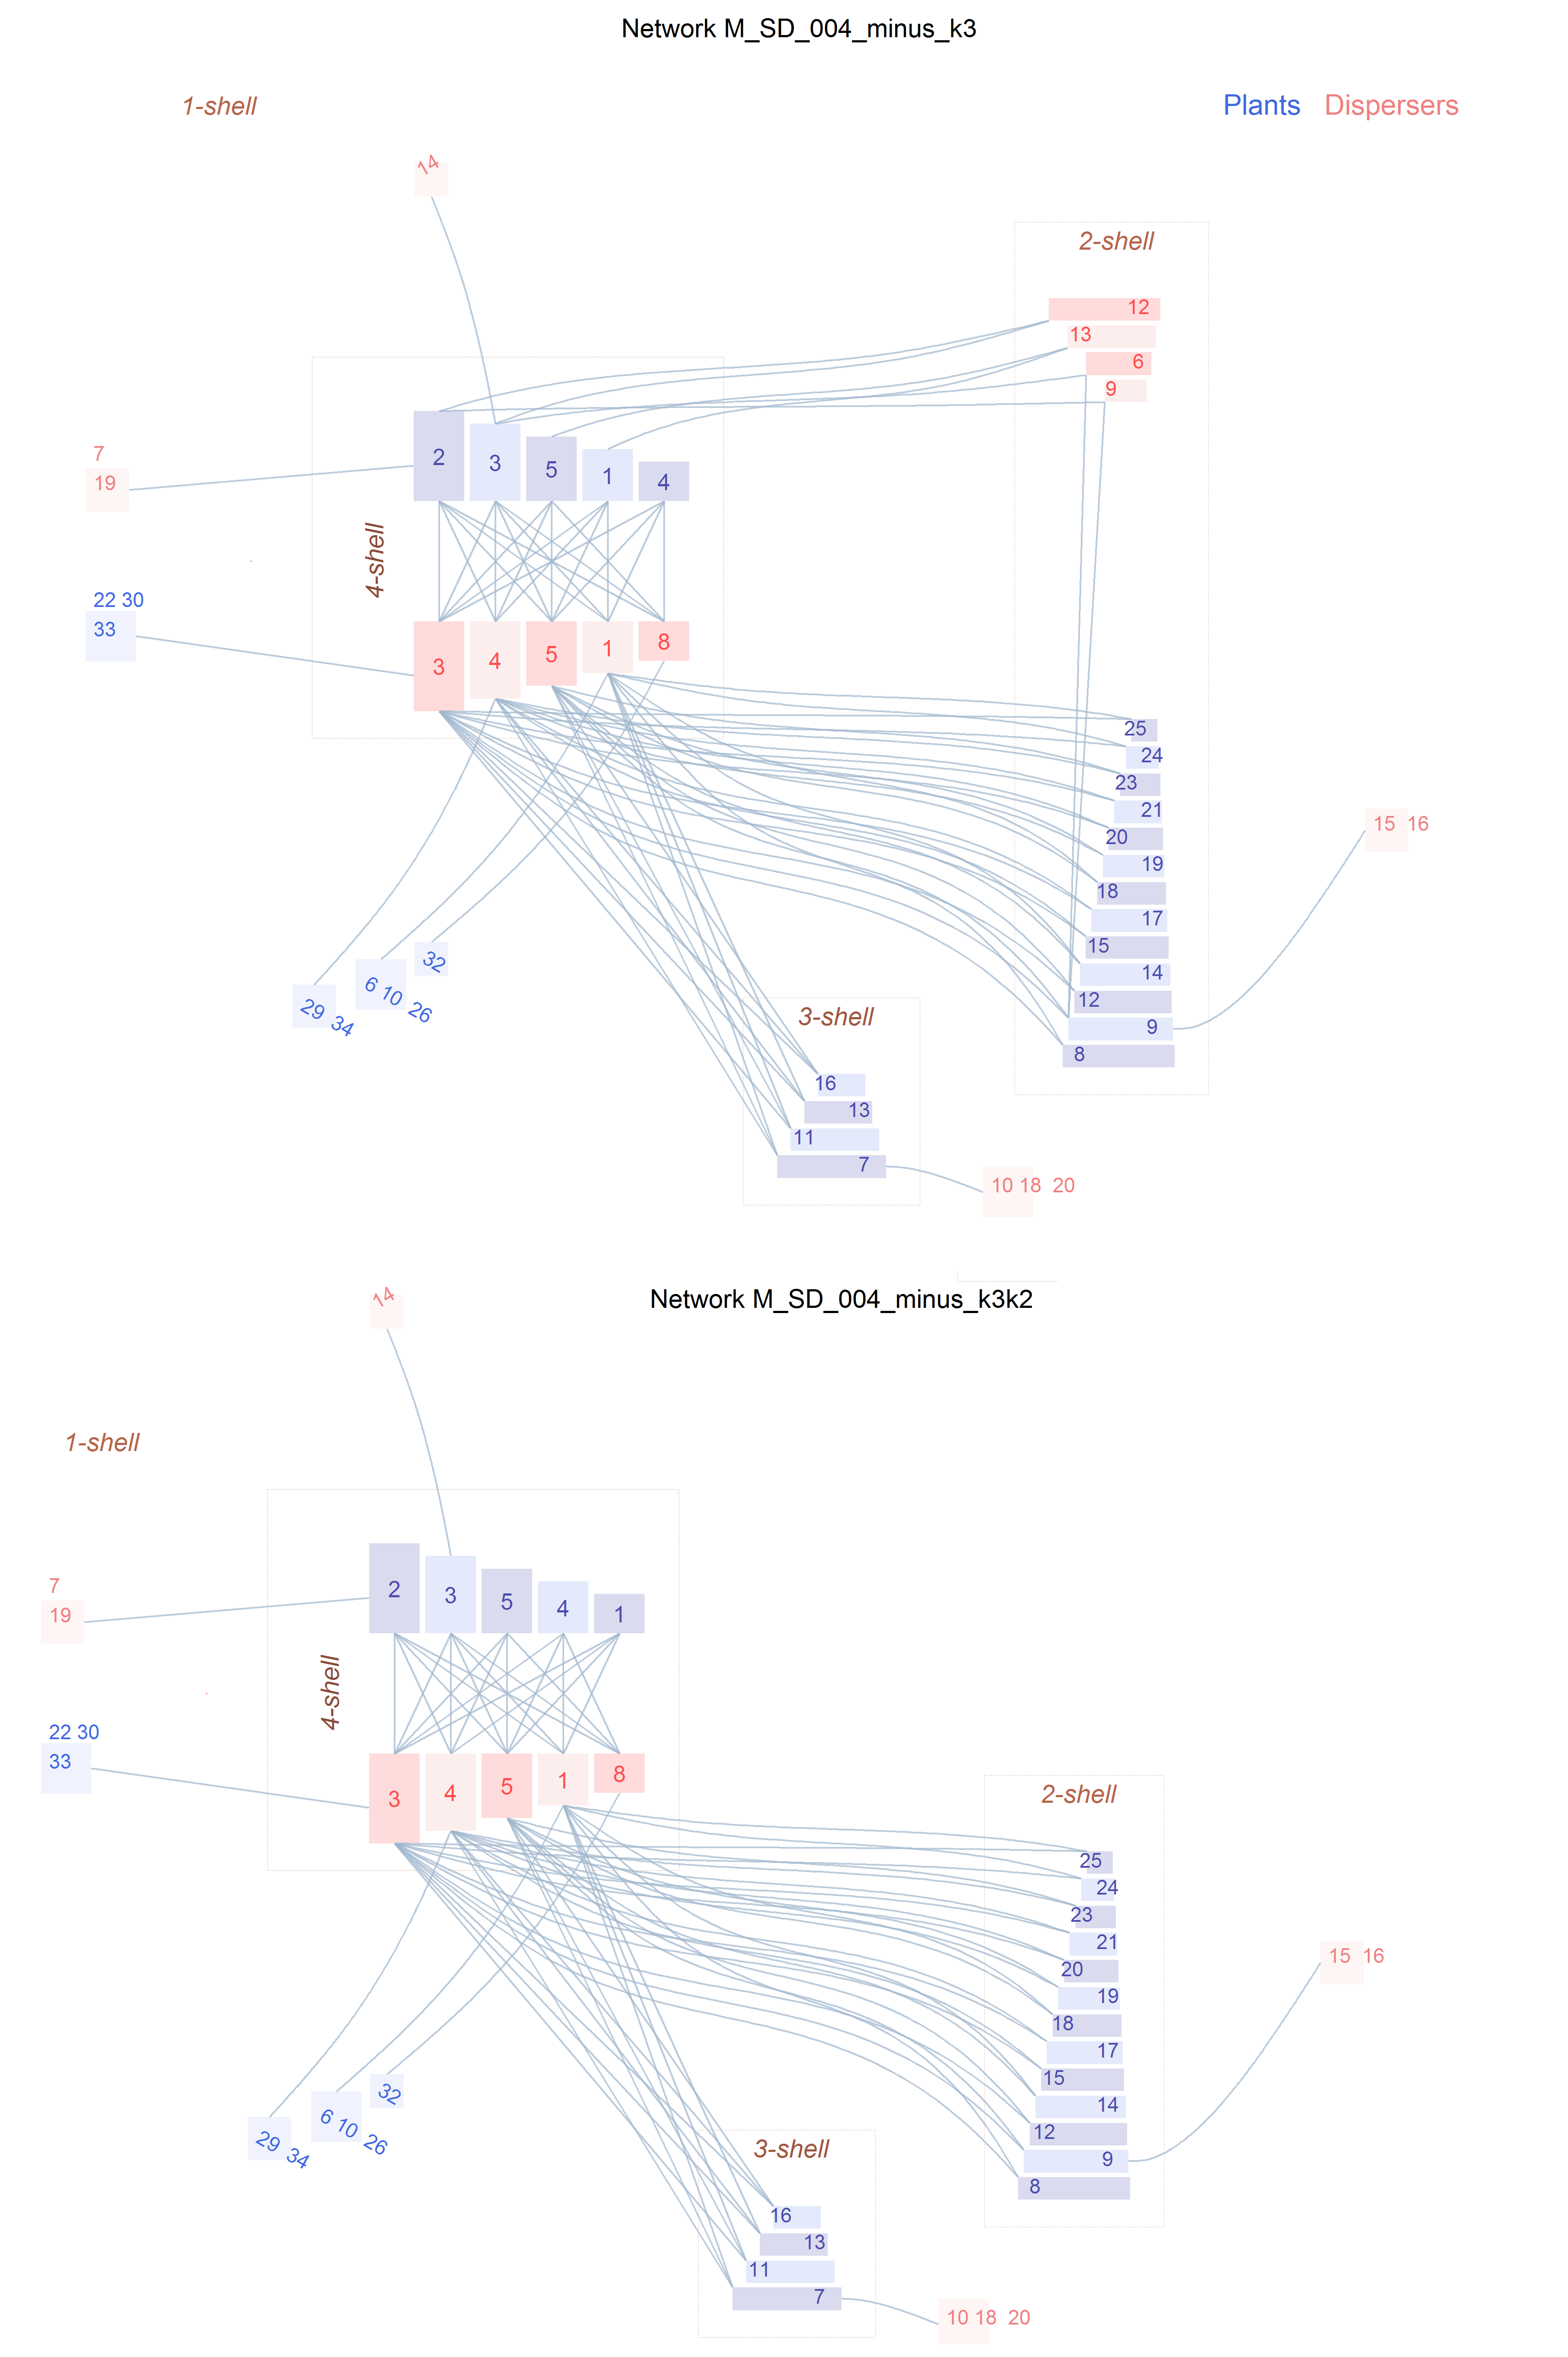
\includegraphics[scale=0.5]{Figures/VIS_M_SD_004_minus_k3k2_ziggurat.png}
\caption {Red de frugívoros $M\_SD\_004$, en la que se han eliminado todos los polinizadores de la $3$-$shell$ ($NODF = 36,24$, $\overline k_{radius} = 2,17$)y la $2$-$shell$ ($NODF = 33,055$, $\overline k_{radius} = 2,15$), véase la figura \ref{fig:ziggurat}.} 
\label{fig:VIS_M_SD_004_minus_k3k2_ziggurat}
\end{figure}

\clearpage
Cabe preguntarse si las redes resultantes de las extinciones se parecen a redes reales. La de toda la colección cuyos parámetros se acercan más a la de la figura \ref{fig:VIS_M_SD_004_minus_k4_ziggurat} es una comunidad de frugívoros que en estado natural tiene un $k$ máximo $2$ (figura \ref{fig:VIS_M_SD_018_ziggurat}). Se ha señalado en el gráfico de correlación de \ref{fig:VIS_Modvskdegree3-sd04} la posición de esta red.

Su aspecto general es muy similar al de lo que queda de la comunidad de Puerto Rico al extinguirse los frugívoros de la \textit{shell} máxima. Esto lleva a pensar que las comunidades mutualistas con índices $k$ máximos menores pueden ser restos de otras anteriores más complejas que han perdido parte de sus nodos. Alternativamente, podrían ser estados iniciales de formación.

Al exponer en el capítulo anterior el mecanismo de extinción basado en $k$-$shell$, se vio que la mayor destrucción se produce si se eliminan éstas de mayor a menor índice. Se ha comprobado como afecta a la red $M\_SD\_004$ la pérdida de los cinco frugívoros de la \textit{shell} máxima, ¿qué ocurre si ese núcleo se mantiene y se destruyen los de índices $k$ menores?

En la imagen superior de la figura \ref{fig:VIS_M_SD_004_minus_k3k2_ziggurat}, se han extinguido las dos especies de frugívoros que formaban la $3$-$shell$. La $NODF$ baja muy poco, de $39,82$ a $36,34$ y el $\overline k_{radius}$ prácticamente no se modifica. El contraste es grande si se compara con el resultado de eliminar los dos frugívoros de mayor $\overline k_{degree}$, tanto en el porcentaje de cambio de las magnitudes como en el de la estructura de la red. Se sigue conservando el índice $k$ máximo $4$.

Si a continuación se extinguen las cuatro especies animales de la $2$-$shell$, tampoco se observan grandes cambios en los parámetros de la red resultante (figura \ref{fig:VIS_M_SD_004_minus_k3k2_ziggurat}, abajo). Esto es así porque los frugívoros desaparecidos tenían casi todos sus enlaces con la $4$-$shell$ de plantas, como consecuencia del anidamiento. Apenas hay arrastre de otras especies (solo las dos plantas de la $1$-$shell$ conectadas a la $3$-$shell$ de animales).

Con este ejemplo se puede entender mejor la importancia del orden de extinción basado en el índice $k$. Si se conservan las \textit{shells} máximas y la red está bien anidada, la pérdida de otras \textit{shells} de índice inferior no arrastra apenas otras especies. Por el contrario, si hay muchos enlaces entre entre estas \textit{shells} inferiores, el fenómeno puede propagarse dando origen a las extinciones en cascada.

La conservación de las especies de las \textit{shells} máximas debe ser prioritaria porque de ellas depende en gran medida la supervivencia de toda la comunidad, y el diagrama zigurat es una ayuda gráfica para la comprensión de este hecho.

\clearpage
\section{Conclusiones}

Nunc posuere quam at lectus tristique eu ultrices augue venenatis. Vestibulum ante ipsum primis in faucibus orci luctus et ultrices posuere cubilia Curae; Aliquam erat volutpat. Vivamus sodales tortor eget quam adipiscing in vulputate ante ullamcorper. Sed eros ante, lacinia et sollicitudin et, aliquam sit amet augue. In hac habitasse platea dictumst.
